\documentclass[a4paper,12pt]{article}
\usepackage{cmap}
\usepackage{amssymb}
\usepackage{amsmath}
\usepackage[T2A]{fontenc}
\usepackage[utf8]{inputenc}
\usepackage[russian]{babel}
\usepackage{indentfirst}
\usepackage{epigraph}
\renewcommand{\epigraphsize}{\small}
% \pagestyle{empty}

\usepackage[left=1.5cm,right=1.5cm,
    top=2cm,bottom=2cm]{geometry}
\usepackage{graphicx}
\graphicspath{ {./images/} }
\newcommand{\RomanNumeralCaps}[1] {\MakeUppercase{\romannumeral #1}}

\newcommand{\mysection}[2]{\setcounter{section}{#1}\addtocounter{section}{-1}\section{#2}}

\setcounter{secnumdepth}{0} 

\linespread{1.15}                          % коэффициент межстрочного интервала
\setlength{\parskip}{0.4em}                % вертик. интервал между абзацами
\binoppenalty=1000 

\usepackage{graphicx}%Вставка картинок правильная
\usepackage{float}%"Плавающие" картинки
\usepackage{wrapfig}%Обтекание фигур (таблиц, картинок и прочего)

\DeclareRobustCommand{\svdots}{% s for `scaling' - знак кратности выровненный по высоте букв
  \, \vcenter{%
    \offinterlineskip
    \hbox{.}
    \vskip0.25\normalbaselineskip
    \hbox{.}
    \vskip0.25\normalbaselineskip
    \hbox{.}%
  }% 
  \,
}
\usepackage{listings}
\usepackage[unicode, pdftex]{hyperref}
\usepackage{xcolor}

\definecolor{linkcolor}{HTML}{50006b} % цвет ссылок
%\definecolor{urlcolor}{HTML}{107896} % цвет гиперссылок
\definecolor{urlcolor}{HTML}{50006b} % цвет гиперссылок
 
\hypersetup{pdfstartview=FitH,  linkcolor=linkcolor,urlcolor=urlcolor, colorlinks=true}

\definecolor{codegreen}{rgb}{0,0.6,0}
\definecolor{codegray}{rgb}{0.5,0.5,0.5}
\definecolor{codepurple}{rgb}{0.58,0,0.82}
\definecolor{backcolour}{cmyk}{0,0,0,0.05}

\lstdefinestyle{mystyle}{
    backgroundcolor=\color{backcolour},
    commentstyle=\color{codegreen},
    keywordstyle=\color{magenta},
    numberstyle=\tiny\color{codegray},
    stringstyle=\color{codepurple},
    basicstyle=\ttfamily\footnotesize,
    breakatwhitespace=false,
    breaklines=true,
    captionpos=b,
    keepspaces=true,
    numbers=left,
    numbersep=5pt,
    showspaces=false,
    showstringspaces=false,
    showtabs=false,
    tabsize=2,
    texcl=true
}

\lstset{extendedchars=\true, style=mystyle}

\usepackage[pages = some]{background}
\backgroundsetup{
	scale = 1,
	angle = 0,
	opacity = 1,
	contents = {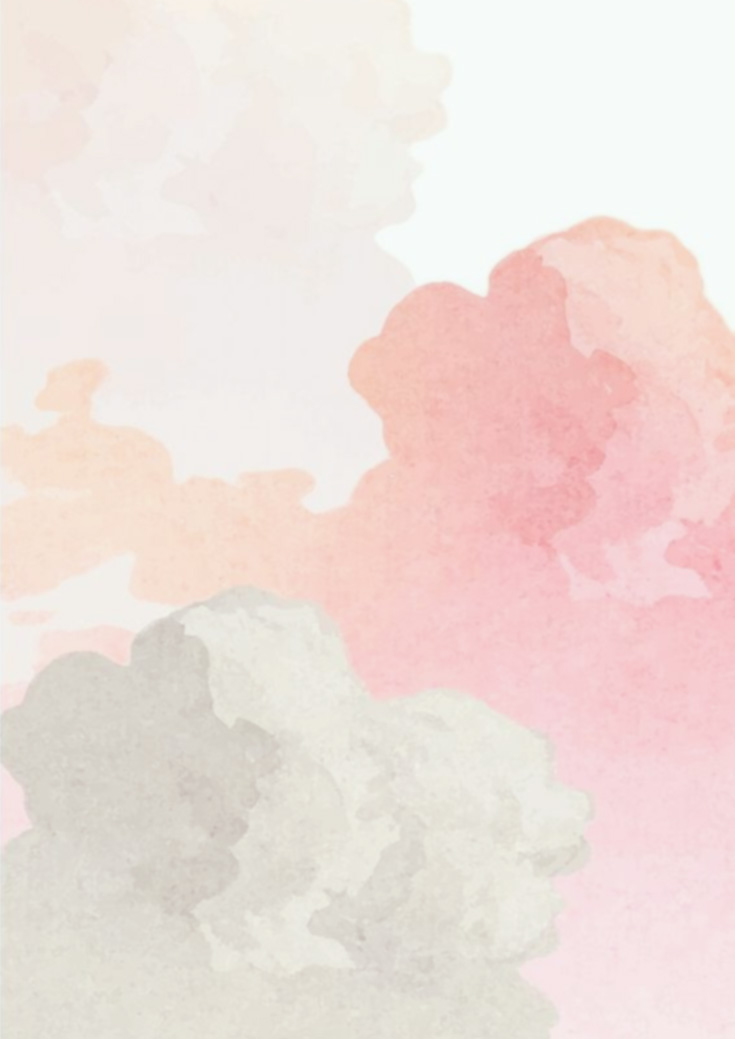
\includegraphics[height = \paperheight, keepaspectratio]{background.jpg}}}
	

% нужно для стрелочки в билете 5.21
\newcommand{\leftrarrows}{\mathrel{\raise.75ex\hbox{\oalign{%
  $\scriptstyle\leftarrow$\cr
  \vrule width0pt height.5ex$\hfil\scriptstyle\relbar$\cr}}}}
\newcommand{\lrightarrows}{\mathrel{\raise.75ex\hbox{\oalign{%
  $\scriptstyle\relbar$\hfil\cr
  $\scriptstyle\vrule width0pt height.5ex\smash\rightarrow$\cr}}}}
\newcommand{\Rrelbar}{\mathrel{\raise.75ex\hbox{\oalign{%
  $\scriptstyle\relbar$\cr
  \vrule width0pt height.5ex$\scriptstyle\relbar$}}}}
\newcommand{\longleftrightarrows}{\leftrarrows\joinrel\Rrelbar\joinrel\lrightarrows}

\makeatletter
\def\leftrightarrowsfill@{\arrowfill@\leftrarrows\Rrelbar\lrightarrows}
\newcommand{\xleftrightarrows}[2][]{\ext@arrow 3399\leftrightarrowsfill@{#1}{#2}}
\makeatother


\newcommand{\Def}{\textbf{Опеределение:} }  % объявление новых макрокоманд
\newcommand{\Statement}{\textbf{Утверждение:} }
\newcommand{\Lemma}{\textbf{Лемма:} }
\newcommand{\Th}{\textbf{Теорема:} }
\newcommand{\Task}{\textbf{Задача:} }
\newcommand{\Solution}{\textbf{Решение:} }
\newcommand{\Example}{\textbf{Пример:} }
\newcommand{\Note}{\textbf{Замечание:} } 
\newcommand{\Vars}{\textbf{Введем обозначения:} } 
\newcommand{\Proof}{$\blacktriangle$ }
\newcommand{\EndProof}{$\blacksquare$ }
\newcommand{\N}{\mathbb{N}}

\newcommand{\Le}{\leqslant}                % русский стиль нестрогих неравенств
\newcommand{\Ge}{\geqslant}
\newcommand{\brackets}[1]{\left({#1}\right)} % автоматический размер скобочек

\newcommand{\angles}[1]{\left\langle{#1}\right\rangle}
\newcommand{\abs}[1]{\left|{#1}\right|}
\newcommand{\bracketss}[1]{\left({#1}\right)}


\newcommand{\drawsome}[1]{
    \begin{figure}[h!]
            \centering
            \includegraphics[scale=0.7]{#1}
            \label{fig:first}
    \end{figure}
}

\newcommand{\drawsomebig}[1]{
    \begin{figure}[h!]
            \centering
            \includegraphics[scale=1.15]{#1}
            \label{fig:first}
    \end{figure}
}

\newcommand{\drawsomemedium}[1]{
    \begin{figure}[h!]
            \centering
            \includegraphics[scale=0.45]{#1}
            \label{fig:first}
    \end{figure}
}

\newcommand{\drawsomesmall}[1]{
    \begin{figure}[h!]
            \centering
            \includegraphics[scale=0.3]{#1}
            \label{fig:first}
    \end{figure}
}

\begin{document}
% ================ ПЕРВАЯ СТРАНИЦА ==========================
    \thispagestyle{empty}
    \BgThispage
    \begin{center}
        \vspace*{4cm}
        
        \Huge
        \textbf{Формальные языки и трансляции} \\
        \textbf{3 семестр} \\
        \textbf{Лектор: Ахтямов П.И.} \\
        \textbf{осень 2021} \\
    
        
        \vspace{7cm}
        \Large
        \textbf{Авторы билетов (лучшие котики):} \\
        \href{https://vk.com/spitsynn}{Спицын Николай} \\
        \href{https://vk.com/dimasav123}{Савичев Дмитрий} \\
        \href{https://vk.com/id165779384}{Подзорова Полина} \\
        \href{https://vk.com/poli.dobro}{Чубенко Полина} \\
        \href{https://vk.com/id340504554}{Клячин Артемий} \\
        \href{https://vk.com/meraklim}{Климанова Ирина} \\
        \href{https://vk.com/ulegor}{Сбродов Егор} \\
        
    \end{center}

\newpage

\tableofcontents
\newpage

% ===================== НАЧАЛО ======================
\mysection{1}{1. Автоматы и регулярки}
    \section{Асимптотические обозначения: $O, \Omega, \Theta$. Независимость от стартового индекса. Мастер-теорема (б/д).}
\par \textbf{Определение:} Пусть $f,g: \; \mathbb{N} \rightarrow \mathbb{N}$. Тогда $f=O(g)$, если существует $c, N$, такие что $\forall n \in N \; \hookrightarrow n \geqslant N \Rightarrow f(n) \leqslant c \cdot g(n)$.
\par \textbf{Определение:} Пусть $f,g: \; \mathbb{N} \rightarrow \mathbb{N}$. Тогда $f=\Omega(g)$, если существует $c, N$, такие что $\forall n \in N \; \hookrightarrow n \geqslant N \Rightarrow f(n) \geqslant c \cdot g(n)$.
\par \textbf{Замечание:} $f = \Omega(g) \Leftrightarrow g = O(f)$
\par \textbf{Определение:} Пусть $f,g: \; \mathbb{N} \rightarrow \mathbb{N}$. Тогда $f=\Theta(g)$, если существует $c_1,c_2, N$, такие что $\forall n \in N \; \hookrightarrow \\ n \geqslant N \Rightarrow c_1 \cdot g(n) \leqslant f(n) \leqslant c_2 \cdot g(n)$.
\par \textbf{Замечание:} $f = \Theta(g) \Leftrightarrow f = O(g)$ и $f = \Omega(g)$
\par \textbf{Утверждение:} $f = O(g) \Leftrightarrow \exists c: \forall n \in \mathbb{N} \hookrightarrow f(n) \leqslant c \cdot g(n)$ 
\par \begin{itemize}
    \item[$\blacktriangle \Leftarrow$] Очевидно, достаточно положить $N=1$
    \item[$\Rightarrow$] Пусть $\forall n \geqslant N \hookrightarrow f(n) \leqslant c \cdot g(n)$. Определим $c'=\max \{c, \frac{f(1)}{g(1)}, \ldots, \frac{f(N)}{g(N)}\}$ ($g$ не обращается в 0 так как результат натуральный). Тогда \begin{enumerate}
        \item $n \geqslant N \Rightarrow f(n) \leqslant c \cdot g(n) \leqslant c' \cdot g(n)$
        \item $n < N \Rightarrow c' \geqslant \frac{f(n)}{g(n)} \Rightarrow f(n) \leqslant c' \cdot g(n) \; \blacksquare$
    \end{enumerate}
\end{itemize}
\par Для $\Omega$ и $\Theta$ справедливы аналогичные утверждения.
\par \textbf{Мастер-теорема (с лекции):} Пусть $T: \mathbb{N} \rightarrow \mathbb{N}$ с условием $T(n)=a \cdot T(\frac{n}{b})+f(n)$, $a=const, a \geqslant 1; \\ b=const, b \geqslant 1, f: \mathbb{N} \rightarrow \mathbb{N}$. Тогда \begin{enumerate}
    \item Если $\exists \varepsilon > 0$, такое что $f(n)=O(n^{\log_b a - \varepsilon})$, то $T(n)=\Theta(n^{\log_b a})$
    \item Если $f(n)=\Theta(n^{\log_b a})$, то $T(n)=\Theta(n^{\log_b a} \log n)$
    \item Если $\exists \varepsilon > 0$, такое что $f(n)=\Omega(n^{\log_b a + \varepsilon})$, причем $\exists c < 1$, такое что $a \cdot f(\frac{n}{b}) \leqslant c \cdot f(n)$ для всех $n$, начиная с некоторого номера, то $T(n)=\Theta(f(n))$
\end{enumerate}
\par \textbf{Мастер-теорема (из интернета):} Пусть имеется рекуррентное соотношение:
$$T(n)=\left\{
\begin{array}{ccc}
a \cdot T(\frac{n}{b})+O(n^c), n>1\\
O(1),n=1\\
\end{array}
\right., \text{ где } a \in \mathbb{N}, b \in \mathbb{R}, b>1, c \in R^+.$$

Тогда асимптотическое решение имеет вид: \begin{enumerate}
    \item Если $c>\log_b a$, то $T(n)=O(n^c)$
    \item Если $c=\log_b a$, то $T(n)=O(n^c \log n)$
    \item Если $c<\log_b a$, то $T(n)=O(n^{\log_b a})$
\end{enumerate}
\newpage{}

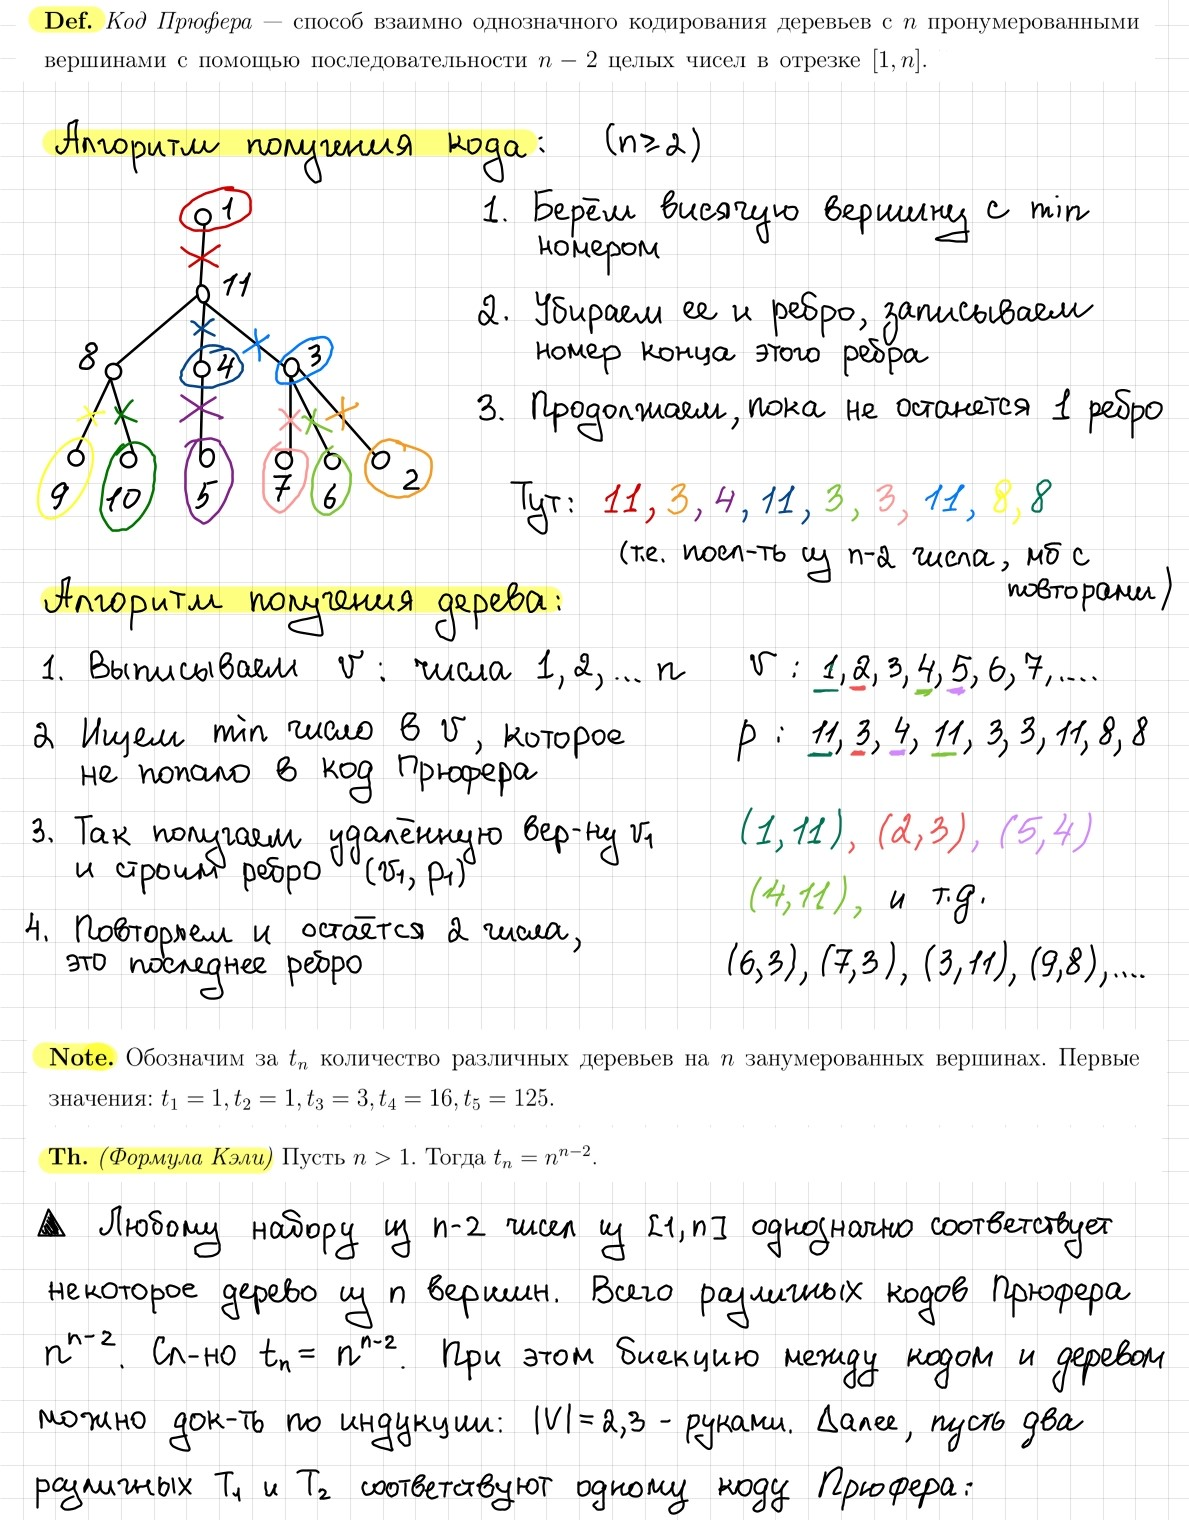
\includegraphics[width=1\linewidth]{sections/Polina/imgs/13.jpg}
\newpage 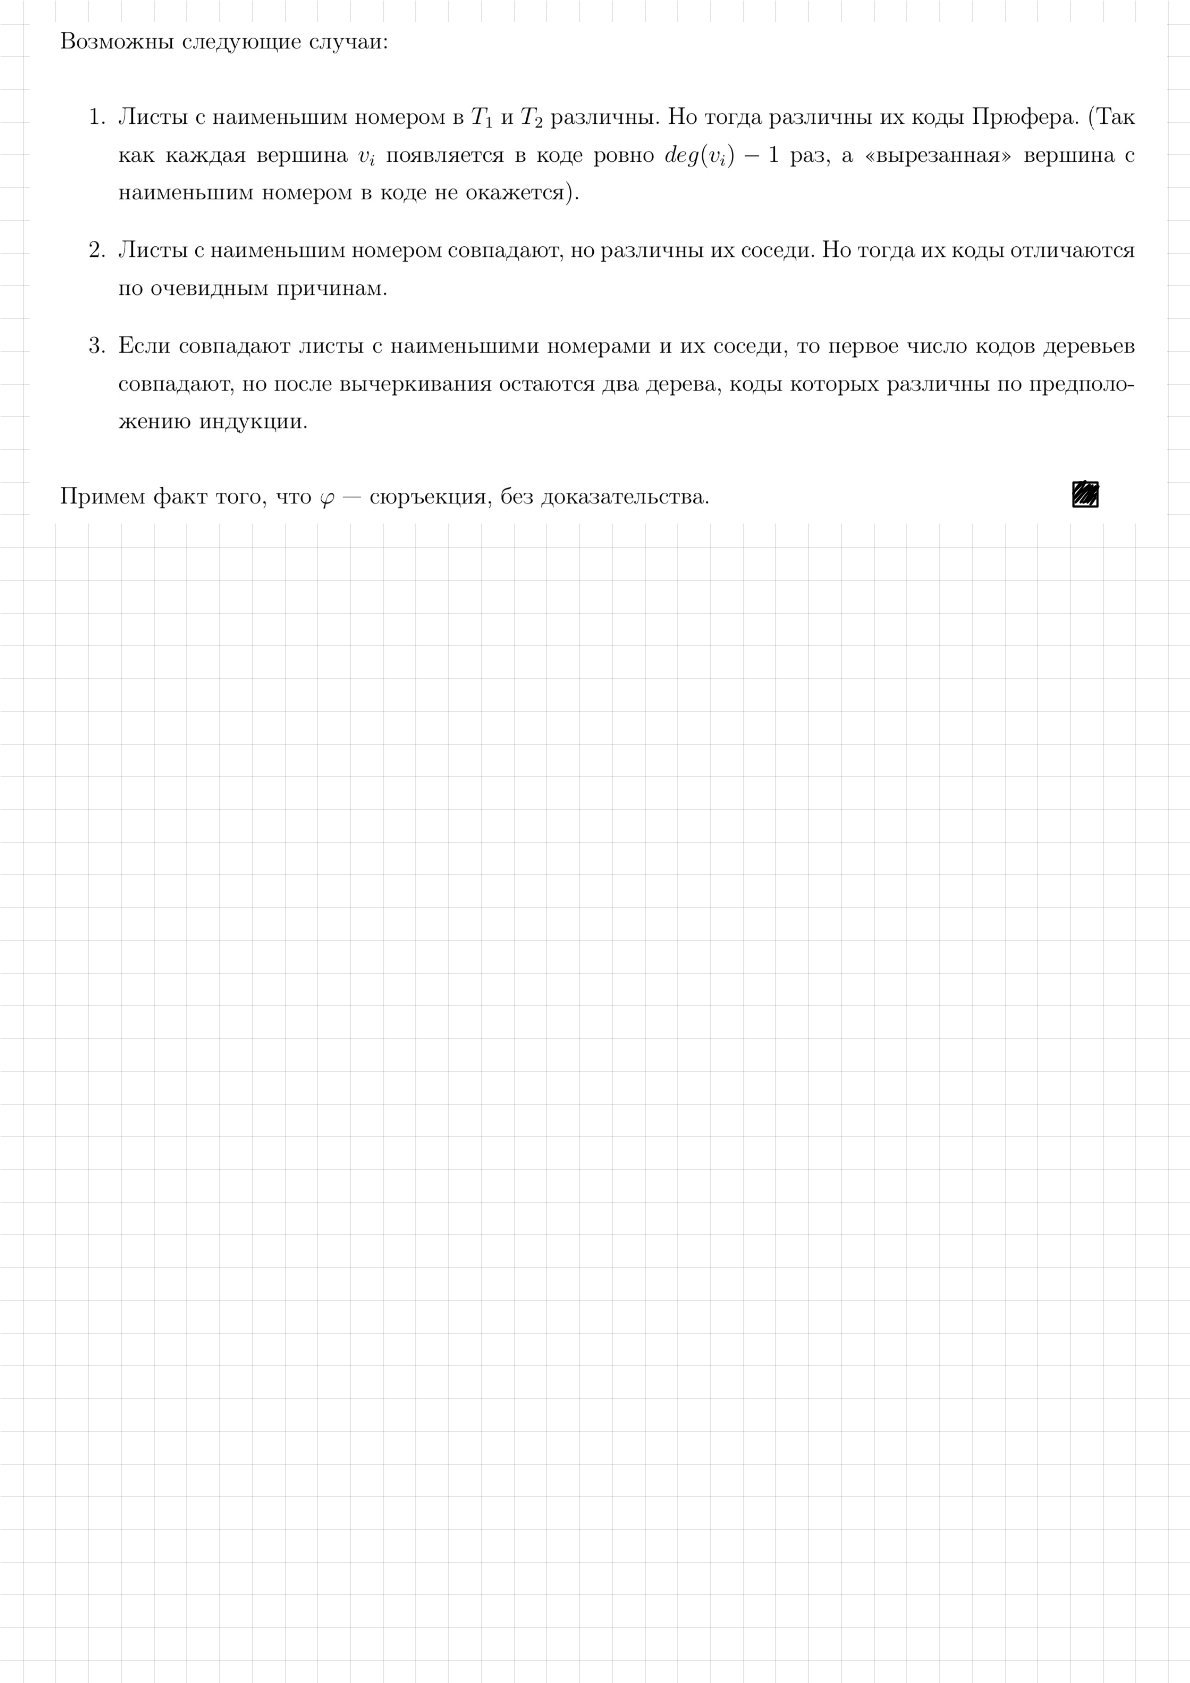
\includegraphics[width=1\linewidth]{sections/Polina/imgs/14.jpg}
\newpage{}

\subsection{3. Свойства класса автоматных языков. Замкнутость относительно булевых операций.}

\Def Полный ДКА.
Полный ДКА (ПДКА) - ДКА, для которого выполнено:
$$\forall a \in \Sigma, q \in Q \,\,\, |\Delta (q, a)| = 1$$

\Statement Для любого автоматного языка $L$ существует ПДКА $M$, такой что $L(M) = M$ (т.е. автоматы распознают одинаковое множество слов);

Метод построения ПДКА из ДКА:\\
1) строим ''стоковую'' вершину.\\
2) Добавляем из всех вершин переходы по недостающим буквам в "сток".

\begin{figure}[h]
    \hspace{-4ex} \begin{minipage}[h]{1\linewidth}
    \center{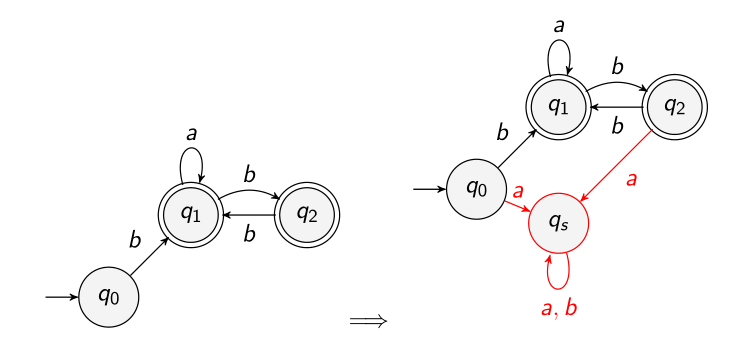
\includegraphics[width=0.6\linewidth]{1_3_1.png}}
    \end{minipage}
    \hspace{-4ex}
\end{figure}

Появятся ли новые слова? - нет, потому что, если мы попали в стоковую вершину, то не сможем ''выбраться'' из неё.

\Def Итерация Клини для языка L.
$$L^* = \cup_{k = 0}^{\infty}L^k$$

\Th Класс автоматных языков замкнут относительно\\
1. Конкатенации\\
2. Объединения\\
3. Пересечения\\
4. Итерации Клини\\
5. Дополнения

\Proof
Далее будем рассматривать только НКА с одним завершающим состоянием.
Для того чтобы после операции у итогового автомата было одно завершающее состояние, добавляем состояние и соединяем завершающие состояния с ним с помощью $\varepsilon$-переходов. (делаем новое состояние - завершающим, а старые - не завершающими)

1) Конкатенация $M_1$ и $M_2$:

Соединяем $\varepsilon$-переходами завершающее состояние $M_1$ со стартовыми состояниями $M_2$.
\begin{center}
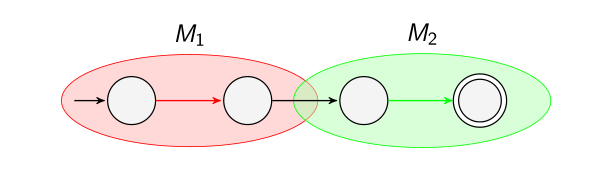
\includegraphics[width=0.45\linewidth]{1_3_2.png}
\end{center}

2) Объединение $M_1$ и $M_2$:

Добавляем стартовое состояние. Соединяем её со стартовыми состояниями $M_1$ и $M_2$ с помощью $\varepsilon$-переходов. 
\begin{center}
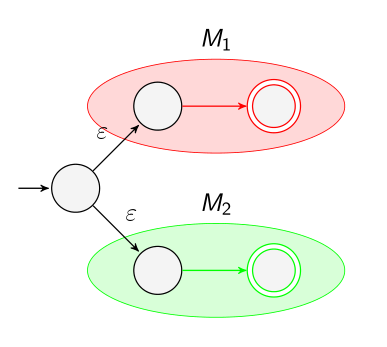
\includegraphics[width=0.25\linewidth]{1_3_3.png}
\end{center}

4) Итерации Клини над $M_1$:

Добавляем стартово-завершающее состояние. С помощью $\varepsilon$-переходов соединяем её с начальными состояниями $M_1$, а завершающее состояния $M_1$ с ней.
\begin{center}
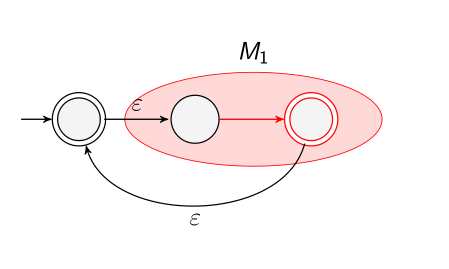
\includegraphics[width=0.32\linewidth]{1_3_4.png}
\end{center}

3) Пересечение $M_1$, $M_2$:

Строим "декартово произведение" автоматов с одно буквенными переходами.

\begin{center}
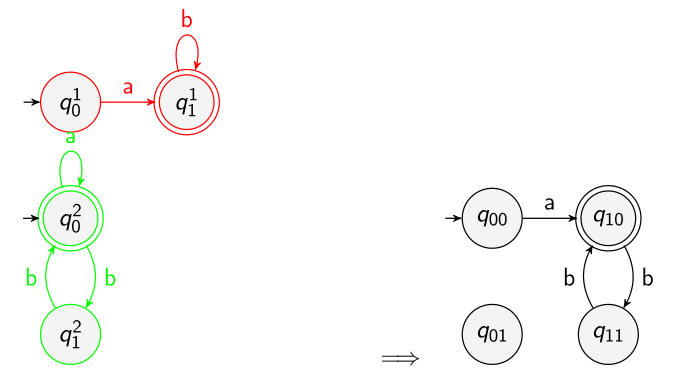
\includegraphics[width=0.55\linewidth]{1_3_5.png}
\end{center}

То есть пересечение будет состоять из состояний, каждому из которых соответствует пара чисел $(i, j)$, это номера состояний из $M_1$ и $M_2$ соответственно, которым это состояние соответствует. И между состояниями $(i_1, j_1)$ и $(i_2, j_2)$ будет проходить ребро с символом $k$, если между $i_1$ и $i_2$ проходило ребро с символом $k$ в $M_1$ и между $j_1$ и $j_2$ проходило ребро с символом $k$ в $M_2$. $(i, j)$ - стартовое состояние, если $i$ - стартовое в $M_1$, $j$ - стартовое в $M_2$. Аналогично с завершающем состоянием. 

5) Дополнение: строим ПДКА и инвертируем терминальность всех состояний.

\newpage{}

\subsection{4. Регулярные выражения. Теорема Клини о совпадении классов регулярных и автоматных языков. Регулярный автомат, алгоритм построения.}

\Vars \\
Regex (регулярное выражение) обозначим за $R$, \newline Language (язык) -- за $L$, \newline $L(R_i)$ (язык, который задается регулярным выражением $R$) -- $L_i$.

\Def Рекурсивное определение регулярного выражения.

% \begin{minipage}[r]{0.1\linewidth} 
% %\begin{flushright}
%     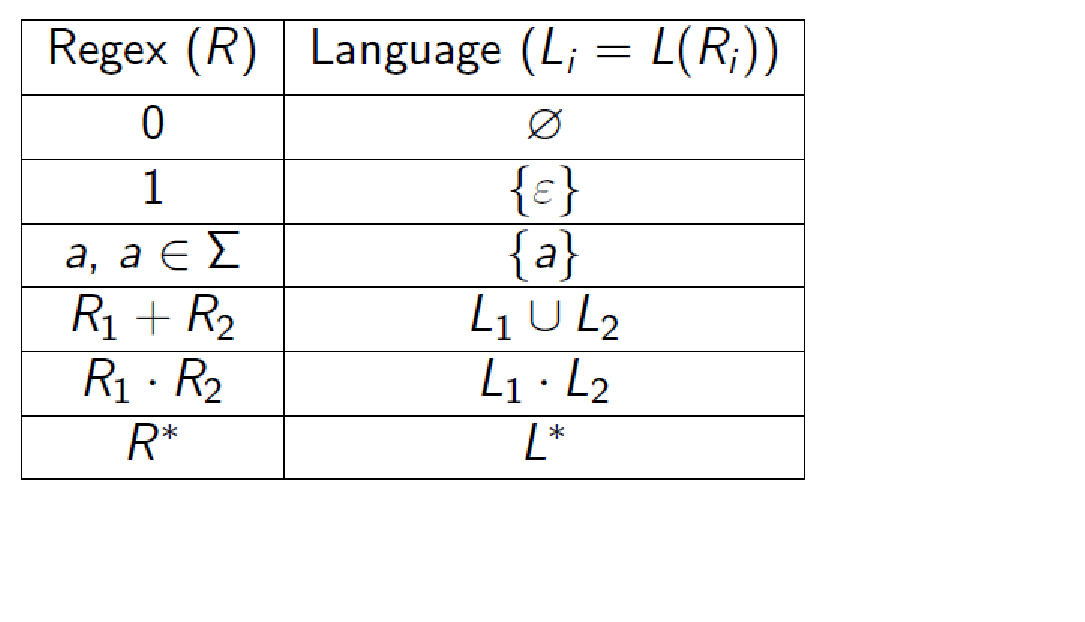
\includegraphics[width=5\linewidth]{images/1_4_1.png}
% %\end{flushright} 
% \end{minipage} 
\begin{center}
    \begin{tabular}{|c|c|}
        \hline
        $Regex (R)$ & $Language (L_i = L(R_i))$ \\
        \hline
        $0$ & $\varnothing$ \\
        $1$ & $\{ \varepsilon \}$ \\
        $a$, $a \in \Sigma$ & $\{ a \}$ \\
        $R_1 + R_2$ & $L_1 \cup L_2$ \\
        $R_1 \cdot R_2$ & $L_1 \cdot L_2$ \\
        $R^*$ & $L^*$ \\
        \hline
    \end{tabular}
\end{center}

Здесь $\varepsilon$ -- пустое слово, <<$\cdot$>> -- операция конкатенации языков (в полученном языке $L_1 \cdot L_2$ лежат слова вида $a_1a_2$, где слово $a_1$ лежит в языке $L_1$, а слово $a_2$ лежит в языке $L_2$), <<$*$>> -- звезда Клини.

Напомним определение звезды Клини: $V^* = \bigcup_{i=0}^{\infty} V^i$ 

\textbf{Приоритет операций} в регулярных выражениях (левее — приоритетнее): $* \rightarrow \cdot \rightarrow +$

\Def Язык $L$ -- регулярный, если он задается регулярным выражением.

\hspace{4ex}

\textbf{Теорема Клини:} Классы регулярных и автоматных языков совпадают.

\Proof Докажем два вложения:

\textbf{1. Регулярные $\subseteq$ Автоматные}

% \begin{figure}[h]
%     \begin{minipage}[h]{0.6\linewidth}
%     Индукция по построению выражения. 
    
%     Немного изменим утверждение -- докажем, что по регулярному выражению можно построить НКА с $1$ завершающим состоянием, который задает тот же язык.\\
    
%     \textit{База}: Построим автоматы для регулярных выражений: 0, 1, a.
%     \end{minipage}
%     \hspace{-4ex} \begin{minipage}[h]{0.5\linewidth}
%     \center{\includegraphics[width=0.6\linewidth]{images/4_base.jpg}}
%     \end{minipage}
% \end{figure}
% Регулярное выражение <<$0$>> -- автомат без завершающих состояний.

% Регулярное выражение <<$1$>> -- в автомате, состоящем из одной вершины, стартовая вершина помечается завершающим состоянием.

% Регулярное выражение <<$a$>> -- в автомате две вершины. Вершина номер $0$ стартовая, вершину номер $1$ помечаем как терминальную. Проводим ребро из $0$ в $1$, на котором пишем букву a.

Индукция по построению выражения. Немного изменим утверждение -- докажем, что по регулярному выражению можно построить НКА с $1$ завершающим состоянием, который задает тот же язык.

\textit{База}: Построим автоматы для регулярных выражений: $0, 1, a \in \Sigma$.
% %картинка%
\begin{figure}[h!]
    \centering
    \includegraphics[scale=0.27]{4_base.jpg}
\end{figure}
% \newline \center{\includegraphics[width=0.29\linewidth]{4_base.jpg}}
% \begin{minipage}[r]{1\linewidth} 
% %\begin{flushright}
%     % 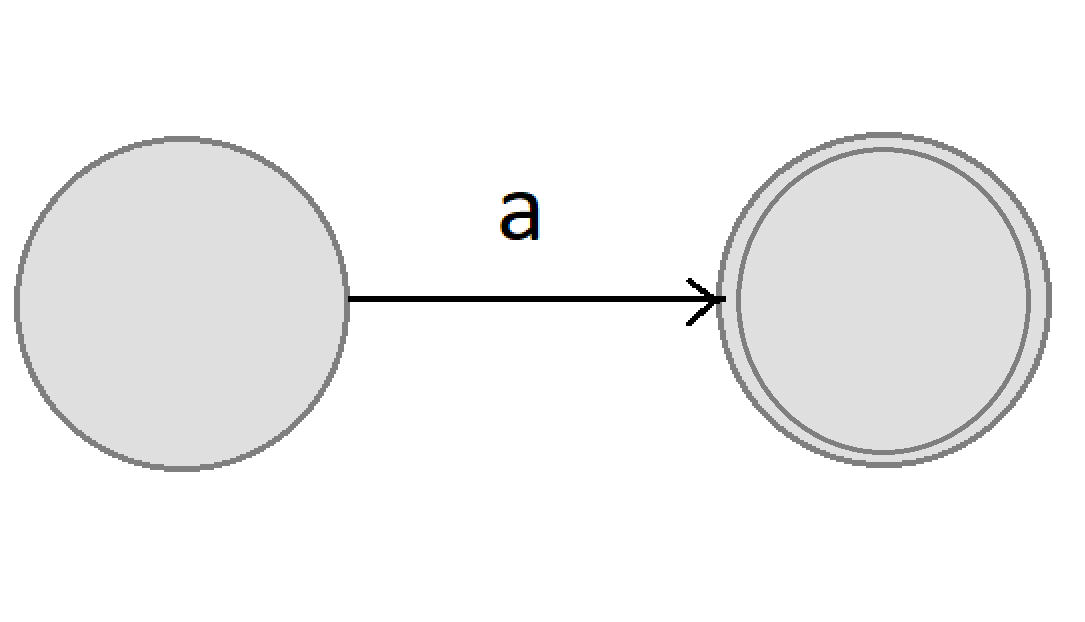
\includegraphics[width=2\linewidth]{images/1_4_2.png}
%     \center{\includegraphics[width=1\linewidth]{images/4_base.jpg}}
% %\end{flushright} 
% \end{minipage} 

\textit{Переход:}

1) $R = R_1 + R_2$. Построим автомат $A_1$ для $R_1$, для которого вершина $S_1$ -- стартовая, а вершина $F_1$ -- единственная терминальная. Для $R_2$ это будут автомат $A_2$ со стартовой вершиной $S_2$ и терминальной $F_2$.
Создадим новую вершину $S$, которая и будет стартовой в новом автомате. Из нее проведем два ребра с $\varepsilon$-переходами в $S_1$ и в $S_2$. Аналогично соединим завершающие в автоматах с новой завершающей вершиной $F$. Нетрудно доказать, что такой автомат задаст тот же язык, что и наше регулярное выражение.

2) $R = R_1 \cdot R_2$. Аналогично прошлому пункту получим автоматы для $R_1$ и $R_2$ с теми же обозначениями. Вершина $S_1$ будет стартовой в нашем новом автомате. Добавим также $\varepsilon$-переход из $F_1$ в $S_2$, уберем терминальность $F_1$.

3) $R = R_1^*$. Построим автомат $A_1$ для $R_1$ со стартовой вершиной $S_1$ и терминальной вершиной $F_1$. Создадим вершину $S$ -- новую стартовую вершину, пометим ее терминальной. Добавим из нее и из $F_1$ $\varepsilon$-переход в $S_1$.

\textbf{2. Автоматные $\subseteq$ Регулярные}

\Note{Регулярный автомат -- НКА, в котором на ребрах записаны регулярные выражения. Докажем утверждение для регулярных автоматов.}

\Note{Всякий НКА задается регулярным автоматом с 1 завершающим состоянием.}

Индукция по $|Q|$ (количеству состояний -- вершин) в регулярном автомате.

\textit{База:}

1) $|Q| = 1$. Тогда в регулярном автомате стартовое состояние является завершающим, и можно однозначно построить регулярное выражение. Такому автомату соответсвует регулярное выражение $a^*$
\newline
\begin{minipage}[r]{0.1\linewidth} 
%\begin{flushright}
    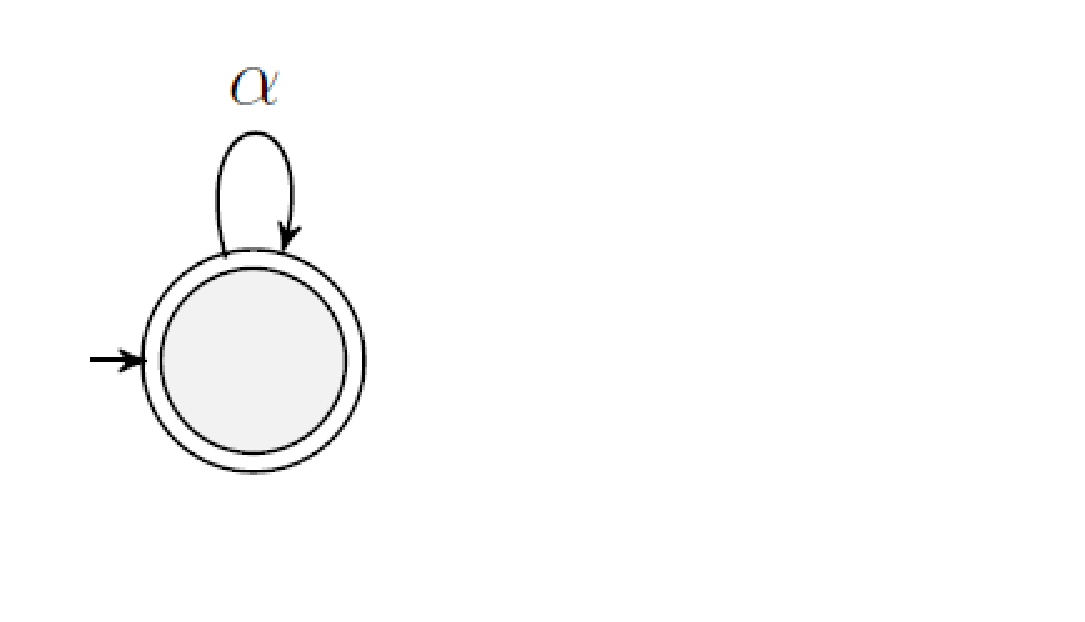
\includegraphics[width=4\linewidth]{images/1_4_3.png}
%\end{flushright} 
\end{minipage} 

2) $|Q| = 2$. Cтартовое состояние и завершающее состояние различны, и можно тоже однозначно построить регулярное выражение. Такому автомату соответсвует регулярное выражение $\alpha^*\beta(\gamma + \delta \alpha^* \beta)^*$
\newline
\begin{minipage}[r]{0.1\linewidth} 
%\begin{flushright}
    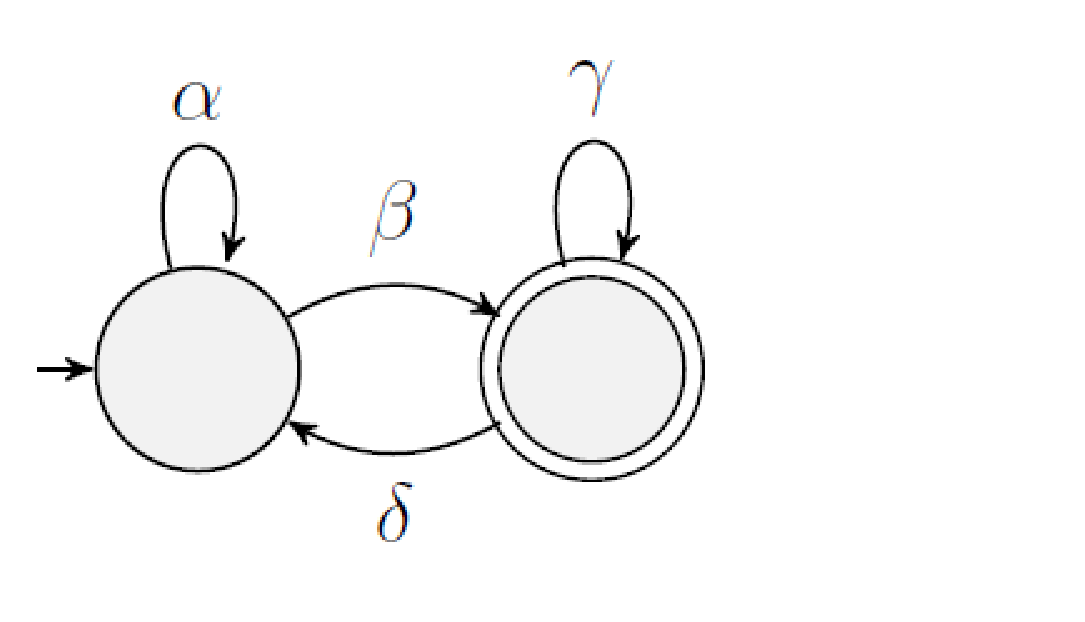
\includegraphics[width=4\linewidth]{images/1_4_4.png}
%\end{flushright} 
\end{minipage} 

Для случая, когда завершающее состояние -- это начальная вершина, регулярное выражение будет $(\gamma + \delta \alpha^* \beta)^*$.

\textit{Переход:}
\Note{Есть нестартовая и незавершающая вершина!}

1) Удаляем кратные ребра:
\begin{minipage}[r]{0.2\linewidth} 
%\begin{flushright}
    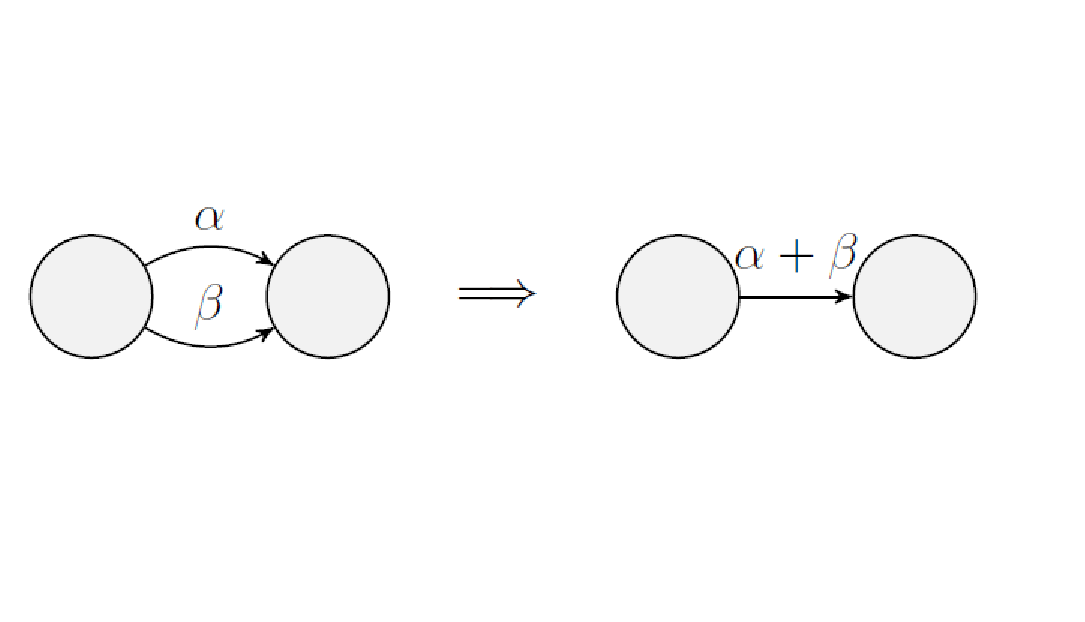
\includegraphics[width=2.5\linewidth]{images/1_4_5.png}
%\end{flushright} 
\end{minipage} 

Кратные ребра означают, что мы можем выбрать, какой символ будем использовать. Именно этот смысл и несет в себе операция <<$+$>>.

2) Добавляем циклы на себя:
\begin{minipage}[r]{0.1\linewidth} 
%\begin{flushright}
    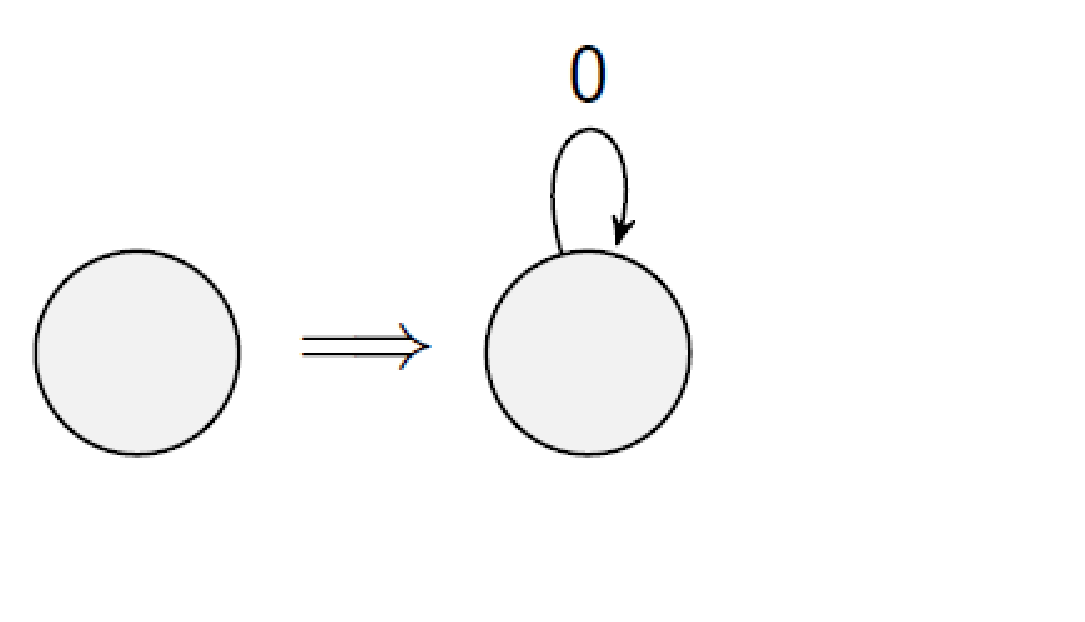
\includegraphics[width=3.5\linewidth]{images/1_4_6.png}
%\end{flushright} 
\end{minipage} 

3) Удаляем нестартовое и незавершающее состояние:

\begin{minipage}[r]{0.1\linewidth} 
%\begin{flushright}
    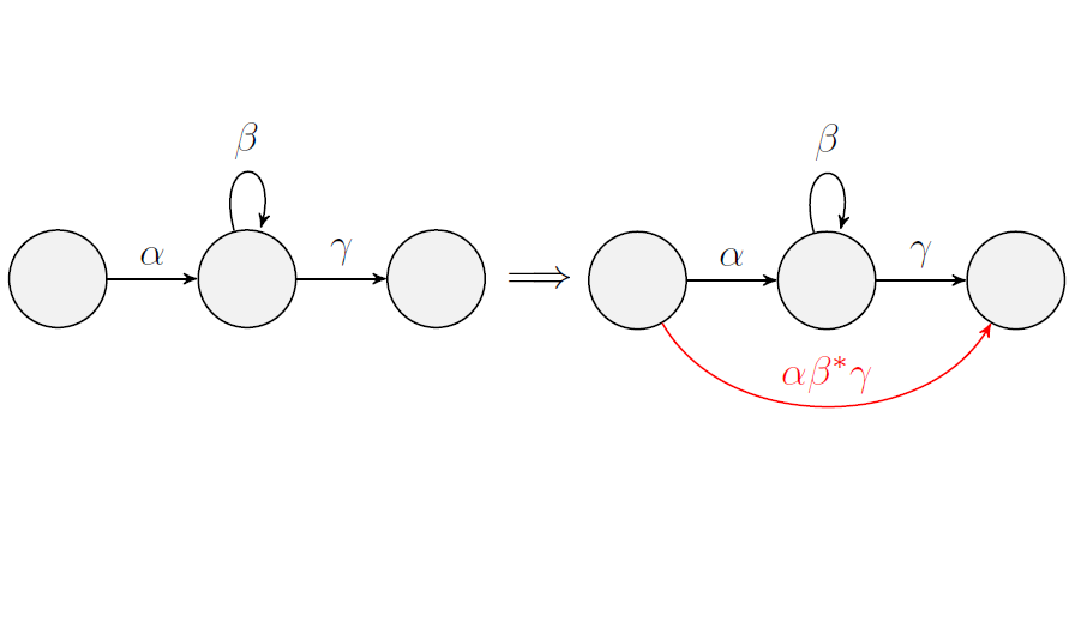
\includegraphics[width=5.5\linewidth]{images/1_4_7.png}
%\end{flushright} 
\end{minipage} 
\newline Теперь у нас на одно сотояние стало меньше, т.е. мы можем воспользоваться утверждением индукции.
\EndProof
\newpage{}

\subsection{5. Минимальный ДКА, его существование.}

\textbf{Мотивировка:} может быть много состояний. А еще не очень понятно, как сравнивать два автомата на эквивалентность. Вернее, если проверять <<в лоб>>, будет долго. Один из способов решить эти проблемы -- минимизация автомата.\\

Пусть $L \subset \Sigma^*$ -- автоматный язык, $M$ -- ПДКА для $L$.

\Def Минимальный ПДКА $M$, распознающий язык $L$, если $M$ -- минимальный по количеству состояний.

\hspace{4ex}

\Def Определим отношение эквивалентности $\sim_L$ на $\Sigma^*:$
$$u \sim_L v \Longleftrightarrow \forall w \in \Sigma^* \,\,(uw \in L \Longleftrightarrow vw \in L)$$

Определение корректно (рефлексивность, симметричность и транзитивность очевидны).

\textit{Множество классов эквивалентности в этом случае:} 
$\Sigma^* /_{\sim_L}:= \{\{u \arrowvert u \sim_L v\} \,\,\arrowvert\,\, v \in \Sigma^*\}$

\Def Определим отношение эквивалентности $\sim_M$ на $Q:$
$$q_1 \sim_M q_2 \Longleftrightarrow \forall w \in \Sigma^*\,\,(\Delta(q_1, w) \in F \Longleftrightarrow \Delta(q_2, w) \in F)$$

Если $q_1 \sim_M q_2$, то состояния можно объединить.

\textit{Напоминание:} Множество вершин, достижимых из $q$ по $w$ -- $\Delta (q, w) = \{ q' | \langle q, w \rangle \vdash \langle q', \varepsilon \rangle \}$..\\

% \hspace{4ex} 
\textbf{Лемма}
Пусть $L_q := \{w \,\arrowvert\, \Delta(q_0, w) = q\}$. Тогда каждый класс эквивалентности в нашем фактор-множестве являетеся объединением классов в $L_q$.

\Proof
Возьмем слово $u \in [u] \in \Sigma^*/_{\sim_L}$, где $[u]$ -- это класс эквивалентности для $u$. Рассмотрим путь по $u$ из $q_0$, а именно,  $q_u = \Delta(q_0, u)$. Для любого слова $w \in [u]$, $q_w = \Delta \brackets{q_0, w}$. Тогда $[u] = \bigcup \limits_{q_w, w \in [u]} L_{q_w}$. Далее докажем, почему это так.
% Из последнего очевидно, что $u \in L_{q_u}$. 

Пусть $v \in [u] \,\Longrightarrow\, v \sim_L u \,\Longrightarrow\, q_v = \Delta \brackets{q_0, v} \,\Longrightarrow\, v \in L_{q_v}$. Тогда $v \in \bigcup \limits_{q_w, w \in [u]} L_{q_w}$.

Пусть $v \in \bigcup \limits_{q_w, w \in [u]} L_{q_w}$. Тогда существует состояние $q_z$, $z \in [u]$, что $v \in L_{q_z} = \{ w | \Delta \brackets{q_0, w} = q_z \}$.
\begin{center}
    $z \in [u] \Longrightarrow z \sim_L u \stackrel{def}{\Longrightarrow} \; \forall w \in \Sigma^* \; \brackets{zw \in L \Longleftrightarrow uw \in L}$
    \begin{equation*}
        \left.
          \begin{array}{ccc}
            v \in L_{q_z} \Longrightarrow & \Delta \brackets{q_0, v} & = q_z \\
            & \Delta \brackets{q_0, z} & = q_z \\
          \end{array}
        \right\} \quad
    \Longrightarrow \quad v \sim_L z \text{ так как $\forall w \in \Sigma^*$ $\Delta \brackets{q_0, vw} \stackrel{(*)}{=} \Delta \brackets{q_0, zw}$}
    \end{equation*}
\end{center}

$\brackets{*}$: $\Delta \brackets{q_0, vw} = \Delta \brackets{\Delta(q_0, v), w} = \Delta \brackets{q_z, w} = \Delta \brackets{\Delta(q_0, z), w} = \Delta \brackets{q_0, zw}$

Так как $v \sim_L z$, $z \in [u]$, то $v \in [u]$. Значит, $[u] = \bigcup \limits_{q_w, w \in [u]} L_{q_w}$, и каждый класс эквивалентности из $\Sigma^* /_{\sim_L}$ — объединение классов в $L_q$. \quad \EndProof

% И так для любого элемента $w \in [u] \hookrightarrow w \in L_{q_w}$. Поэтому \[ [u] \subset \bigcup_{q_w, w \in [u]} L_{q_w}.\]

% Докажем теперь обратное включение. Возьмем $v \in L_{q_w}$. Для него верно $q_v = \Delta(q_0, v) = q_w$. Докажем, что тогда $v \in [w]$ ($[u] = [w]$).

% Возьмем произвольное $m \in \Sigma^*$. Заметим, что тогда верно $vm \in L \Longleftrightarrow wm \in L$, ведь слово $w$ читается из состояния $q_v$ и приводит в завершающее тогда и только тогда, когда то же самое верно и для $q_w$ (просто в силу того, что $q_v = q_w$).


\textbf{Следствие}
$\arrowvert \Sigma^*/_{\sim_L} \arrowvert \leq \arrowvert Q \arrowvert$\\

\textit{Теперь перейдем к минимальному ПДКА, а именно докажем его существование (тут) и единственность с точностью до изоморфизма (билет 6).}\\

\textbf{Лемма} Для любого автоматного языка $L$ существует ПДКА $M'$ такой, что все состояния в $M'$ попарно неэквивалентны.

Что необходимо доказать?\\
1) Переходы и завершающие состояния согласованы\\
2) Распознаваемые языки совпадают\\
3) Состояния попарно неэквивалентны

\Proof Рассмотрим автомат над классами эквивалентности $\sim_M$. Класс эквивалентности $q$ обозначим за $[q]$. $M' = \langle Q /_{\sim_M}, \Sigma, \Delta', [q_0], F' \rangle$, где:

\begin{center}
    $\Delta' = \{ \langle [q_1], a \rangle \rightarrow [q_2] \;|\; \exists \langle q_1, a \rangle \rightarrow q_2 \in \Delta \}$
    
    $F' = \{ [q_f] \;|\; q_f \in F \}$
\end{center}

1) Проверим, что множества $\Delta'$, $F'$ заданы корректно.

Для $\Delta'$: Пусть $q_1 \sim_m q_1'$, и существует $a$ такое, что $\Delta \brackets{q_1, a} \nsim_m \Delta \brackets{q_1', a}$.
\begin{center}
    $q_1 \sim_M q_1' \stackrel{def}{\Longrightarrow} (\forall w \in \Sigma^* \;\;\Delta \brackets{q, w} \in F \Longleftrightarrow \Delta \brackets{q_1', w} \in F)$
    
    $w = au \Longrightarrow (\forall u \in \Sigma^* \;\; \Delta \brackets{q_1, au} \in F \Longleftrightarrow \Delta \brackets{q_1', au} \in F)$
\end{center}

Далее обозначим $\Delta \brackets{q_1, a} = q_2$, a $\Delta \brackets{q_1', a} = q_2'$.
\begin{center}
    $\Delta \brackets{q_1, au} = \Delta \brackets{\Delta(q_1, a), u} = \Delta \brackets{q_2, u}$
    
    $\Delta \brackets{q_1', au} = \Delta \brackets{q_2', u}$
    
    $(\Delta \brackets{q_2, u} \in F \Longleftrightarrow \Delta \brackets{q_2', u} \in F)\; \Longrightarrow q_2 \sim_m q_2'$.
\end{center}

Приходим к противоречию.

Для $F'$:
\begin{center}
    $q_1 \in F$, $q_2 \sim_M q_1 \overset{w = \varepsilon}{\Longrightarrow} (\Delta \brackets{q_1, \varepsilon} \in F \Longleftrightarrow \Delta \brackets{q_2, \varepsilon} \in F)$
    
    Значит, $q_1 \in F \Longleftrightarrow q_2 \in F$
\end{center}

2) Теперь покажем, что $L \brackets{M} = L \brackets{M'}$. 

Для этого нужно показать, что $w \in L \brackets{M} \Longleftrightarrow \Delta \brackets{q_0, w} \in F \stackrel{?}{\Longleftrightarrow} \Delta \brackets{[q_0], w} \in F'$.

Докажем утверждение: $\forall u: \Delta \brackets{q_0, u} = q_1 \Longleftrightarrow \Delta \brackets{[q_0], u} = [q_1]$.

Индукция по длине слова $u$.

\textbf{База.} $|u| = 0 \Longrightarrow u = \varepsilon$. Тогда $\Delta \brackets{q_0, \varepsilon} = q_0$, $\Delta \brackets{[q_0], \varepsilon} = [q_0]$.

\textbf{Переход.} Пусть $u = va$, $v \in \Sigma^*$, $a \in \Sigma$.

\begin{center}
    $\Delta \brackets{q_0, va} = q_1 \Longrightarrow \exists q_2\; \Delta \brackets{q_0, v} = q_2, \;\Delta \brackets{q_2, a} = q_1$
\end{center}

По предположению индукции, $\Delta \brackets{[q_0], u} = [q_2]$, $\Delta \brackets{[q_2], a} = [q_1]$, так как переход $\langle q_2, a \rangle \rightarrow q_1 \in \Delta$ тогда и только тогда, когда $\langle [q_2], a \rangle \rightarrow [q_1] \in \Delta'$. По транзитивности, $\Delta \brackets{[q_0], ua} = [q_1]$.

3) Теперь покажем, что состояния попарно неэквивалентны. В автомате, построенном на классах эквивалентности состояний никакие два состояния не эквивалентны, потому что тогда бы они лежали в одном классе, т.е. были бы одним состоянием.

Пусть $[q_1] \sim_{M'} [q_2]$. Тогда $\forall w : \Delta_{M'} \brackets{[q_1], w} \in F' \Longleftrightarrow \Delta_{M'} \brackets{[q_2], w} \in F'$ по определению. 

\begin{center}
    $[q_{1f}] = \Delta_{M'} \brackets{[q_1], w} \in F'$
    
    $[q_{2f}] = \Delta_{M'} \brackets{[q_2], w} \in F'$
    
    $\exists q_{1f} \in F : \Delta_M \brackets{q_1, w} = q_{1f} \in F \Longleftrightarrow \exists q_{2f} \in F : \Delta_M \brackets{q_2, w} = q_{2f} \in F$
    
    $q_1 \sim_{M} q_2 \Longrightarrow [q_1] = [q_2]$
\end{center}
\begin{flushright}
  \EndProof
\end{flushright} 


\Th $M$ — минимальный ПДКА, распознающий язык $L$, тогда и только тогда, когда любые два состояния попарно неэквивалентны и все состояния достижимы из стартового.

\textit{Теперь запишем более формально:}

\begin{center}
    $M$ — минимальный ПДКА $\Longleftrightarrow \begin{cases} \forall q_1, q_2 \in Q \ q_1 \nsim q_2 \\ \forall q \in Q \ \exists w \in \Sigma^* : \ \langle q_0, w \rangle \vdash \langle q, \varepsilon \rangle \end{cases}$
\end{center}

\Proof

$\Longrightarrow$ Если $q_1 \sim_M q_2$, то $[q_1] = [q_2]$, и их можно объединить в одно состояние, значит, $M$ не был бы минимальным, и тогда из минимальности следует, что $q_1 \nsim_M q_2$. Если среди состояний есть недостижимые, то если их удалить, то множество принимаемых слов не изменится.

$\Longleftarrow$ По следствию из леммы о $L_q$: $|\Sigma^* /_{\sim_L}| \leqslant |Q|$. Рассмотрим $w_1$, $w_2$ такие, что $\Delta \brackets{q_0, w_1} \neq \Delta \brackets{q_0, w_2}$. Введём обозначения:

\begin{center}
    $\Delta \brackets{q_0, w_1} = q_1$
    
    $\Delta \brackets{q_0, w_2} = q_2$
\end{center}

Неэквивалентность состояний $q_1$, $q_2$ означает, что существует слово $w$, что б.о.о:

\begin{center}
    $\Delta \brackets{q_1, w} = \Delta \brackets{q_0, w_1 w} \in F \Longleftrightarrow w_1 w \in L$
    
    $\Delta \brackets{q_2, w} = \Delta \brackets{q_0, w_2 w} \notin F \Longleftrightarrow w_2 w \notin L$
    
    Следовательно, получили что $w_1 \nsim_L w_2$
\end{center}

Тогда для автомата $M$ со множеством состояний $Q'$ выполняется, что $|\Sigma^* /_{\sim_L}| \geqslant |Q'|$, но тогда $|Q| \geqslant |\Sigma^* /_{\sim_L}| \geqslant |Q'|$, и $M$ — минимальный. \quad \EndProof
\newpage{}

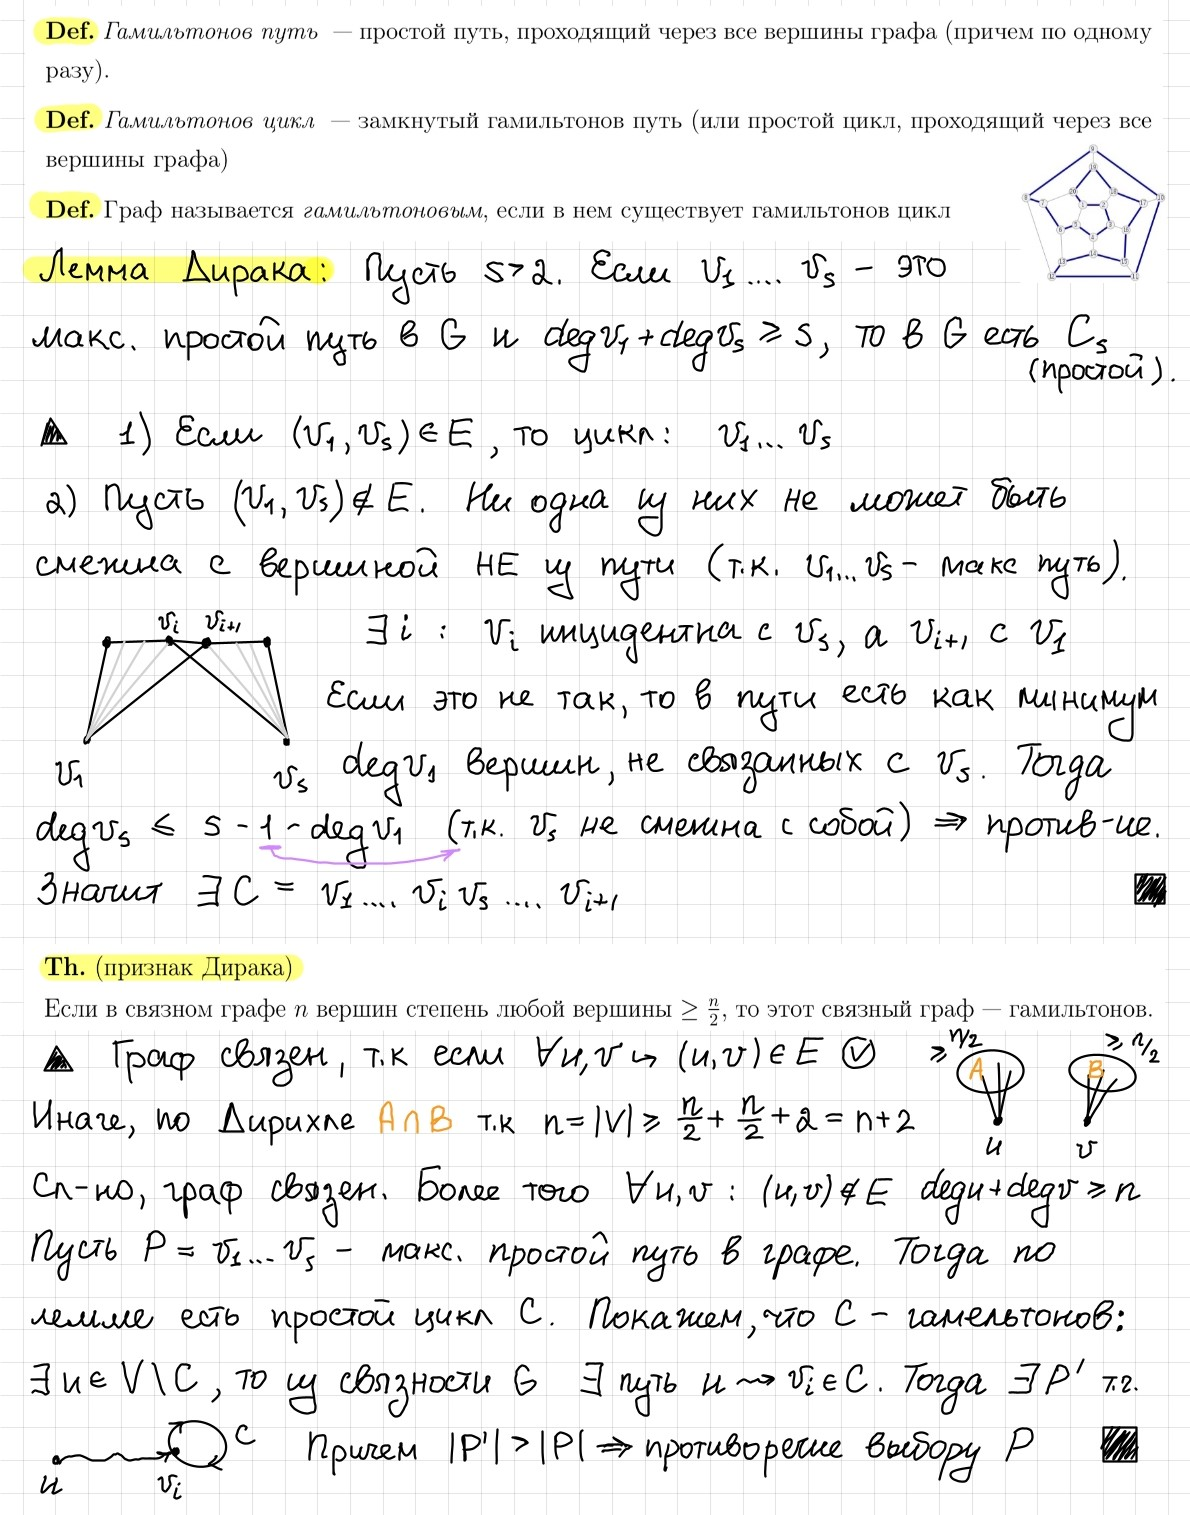
\includegraphics[width=1\linewidth]{sections/Polina/imgs/25.jpg}
\newpage{}

\setcounter{section}{6}

\section{Понятия образа и прообраза множества при соответствии. Критерий равенства образа пересечения и пересечения образов. Аналогичные критерии с объединением и разностью.} 
\textbf{Соответствие} между множествами A и B - произвольное подмножество декартова произведения $F \subset A \times B$. Обозначение: $F: A \to B$; иногда, чтобы подчеркнуть, что одному элементу из A может соответствовать несколько элементов из B, пишут: $F:A\rightrightarrows B$. 
\\
\par
Пусть $F: A \to B$ - соответствие, $S \subset A$, $T \subset B$. Тогда \textbf{образ} множества S - множество всех элементов B, соответствующих какому-то элементу S. Формально: $F(S) = \bigcup_{s \in S} F(s) \subset B $. \textbf{Прообраз} множества Т - множество элементов А, которым соответсвует хотя бы один элемент Т. Формально: $F^{-1}(T) = \left\{ a: F(a) \cap T \neq \varnothing \right\}$ 
\\
\par
\emph{ Образ пересечения любых двух множеств равняется пересечению образов тех же множеств $\iff$ соответствие инъективно. } 
\\
$\blacktriangle$
Пусть соответствие не инъективно. Тогда найдутся такие $a_1$ и $a_2$, что $F(a_1)$ и $F(a_2)$ пересекаются. Тогда $F(\left\{a_1\right\} \cap \left\{a_1\right\}) = F(\varnothing) = \varnothing$, но $F(\left\{a_1\right\}) \cap F(\left\{a_2\right\}) = F(a_1) \cap F(a_2)$ не пуст по предположению. Значит, образ пересечения множеств $\left\{ a_1\right\}$ и $\left\{ a_2\right\}$ не равен пересечению образов. \par
Теперь пусть соответствие инъективно. Рассмотрим произвольные подмножества S и Q множества А. Докажем, что $F(S \cap Q) = F(S) \cap F(Q)$. Для этого докажем включение в обе стороны. Вначале пусть $y \in F(S \cap Q)$. Это значит, что $y \in F(x)$ для некоторого $x \in S \cap Q$. Тогда $x \in S$ и $x \in Q$. А раз $y \in F(x)$, то $y \in F(S)$ и $y \in F(Q)$. Значит, $y \in F(S) \cap F(Q)$. (Это включение верно для всех соответствий). \par
Теперь пусть $y \in F(S) \cap F(Q)$. Значит, $y \in F(x_1)$ для некоторого $x_1 \in S$ и $y \in F(x_2)$ для некоторого $x_2 \in Q$. Но при $x_1 \neq x_2$ в силу инъективности множества $F(x_1)$ и $F(x_2)$ не пересекаются. А их пересечение содержит хотя бы y. Значит, $x_1 = x_2 = x$, и $x \in S \cap Q$. А так как $y \in F(x)$, то получаем $y \in F(S \cap Q)$.
$\blacksquare$ \\
\par
\emph{ Образ объединения любых двух множеств равняется объединению образов тех же множеств - выполняется для любых соответствий. } \\
$\blacktriangle$
1) $\left.
  \begin{array}{ccc}
    A \subseteq A \cup B \Rightarrow F(A) \subseteq F(A \cup B) \\
    B \subseteq A \cup B \Rightarrow F(B) \subseteq F(A \cup B) \\
  \end{array}
\right\} \Rightarrow F(A) \cup F(B) \subseteq F(A \cup B) $ \\
2) $y \in F(A \cup B) \Rightarrow \exists x \in A \cup B: y = F(x) \Rightarrow \exists x \in A \cup x \in B: y = F(x) \Rightarrow$ \\
$\Rightarrow y \in F(A) \cup y \in F(B) \Rightarrow y \in F(A) \cup F(B) \Rightarrow  F(A \cup B) \subseteq F(A) \cup F(B) $; \\
Из пунктов 1 и 2 следует, что $F(A \cup B) = F(A) \cup F(B) $
$\blacksquare$ \\
\par
\emph{ Образ разности любых двух множеств равняется разности образов тех же множеств $\iff$ соответствие инъективно. } \\
Доказательство аналогично доказательству для пересечения.
\newpage{}

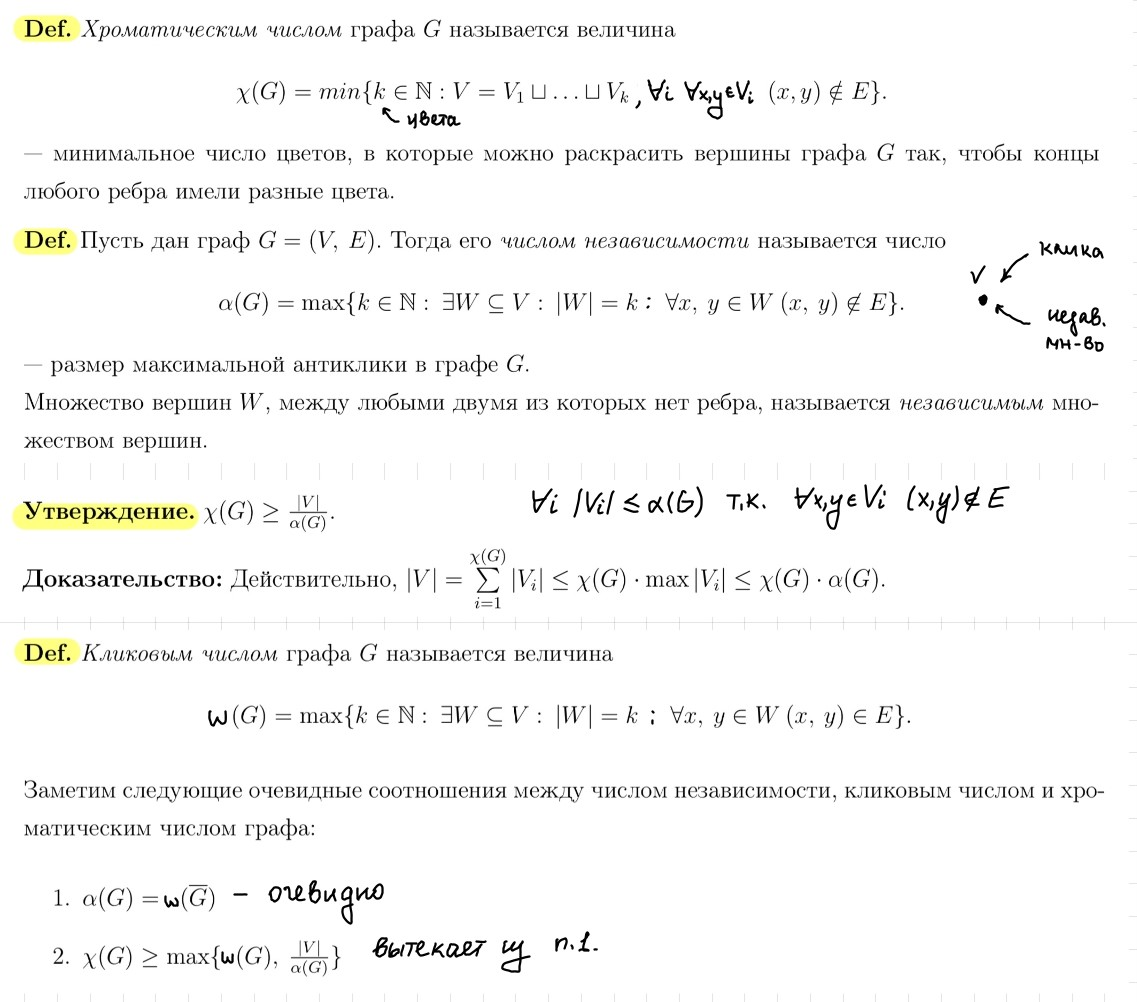
\includegraphics[width=1\linewidth]{sections/Polina/imgs/5.jpg}
\newpage{}

\setcounter{section}{8}
\section{Проверка правильности скобочной последовательности с несколькими типами скобок.}
\par \textbf{Определение}: \textit{Правильные скобочные последовательности с несколькими типами скобок} (рассмотрим с двумя)
\begin{enumerate}
    \item $\varepsilon$ (пустое слово) - ПСП
    \item $S$ - ПСП $\Rightarrow (S), [S]$ - ПСП
    \item $S_1, S_2$ - ПСП $\Rightarrow S_1 S_2$ - ПСП 
\end{enumerate}
\par \textbf{Задача:} Проверить, является ли последовательность из нескольких типов скобок правильной скобочной последовательностью
\par \textbf{Решение:} Храним стек незакрытых открывающих скобок
\lstinputlisting[language=C++,
emph={int,char,double,float,unsigned},
emphstyle={\color{blue}}
]{code/9_psp.cpp}
\par \textbf{Утверждение:} Данный алгоритм корректен, то есть ПСП $\Leftrightarrow$ алгоритм вывел true
\begin{itemize}
    \item[$\blacktriangle \Rightarrow$] Индукция по построению \begin{enumerate}
    \item База: $\varepsilon$ - обработается корректно
    \item $T=(u)$, $u$ - ПСП. По предположению индукции, всё $u$ удалится из стека к моменту прихода закрывающей скобки (можно считать, что стек начинается после первой скобки, она никак не влияет на применение алгоритма к $u$), а внешние скобки обработаются корректно (аналогично для других типов скобок)
    \item $T=T_1 T_2; T_1, T_2$ - ПСП. По предположению индукции, после того как считается $T_1$ стек опустошится $\Rightarrow$ после $T_2$ - тоже $\Rightarrow$ алгоритм сработает корректно $\blacksquare$
    \end{enumerate}
    \item[$\Leftarrow$] Доказываем индукцией по количеству действий, "обращая" предыдущий пункт.
    \par Рассмотрим скобочную последовательность, на которую алгоритм выдаёт true. Алгоритм сопоставил каждой открывающейся скобке одного типа закрывающуюся скобку того же типа. Причём они обязательно идут в правильном порядке. 
\parДля доказательства факта используем индукцию.
Рассмотрим пары соответсвующих скобок в порядке закрытия пары:
\begin{enumerate}
    \item База: Если между парой скобок нет других скобок, то последовательность от одной скобки до другой - правильная.
    \item Шаг: Если между парой скобок (назовём их $a$ и $b$ соответственно) есть непустая подстрока, то все скобки из подстроки уже были рассмотрены индукцией, так как открывающиеся скобки в подстроке были позже, чем $a$ добавлены в стек и по правилу стека должны были раньше из него выйти, а значит они уже были рассмотрены индукцией. Аналогично с закрывающимеся скобками из подстроки - они идут раньше, чем $b$, следовательно, по правилу стека им ставили в соответствие открывающиеся скобки, которые были добавленны позже $a$. (окрывающаяся скобка не могла быть добавленны раньше $a$, потому что $a$ перегородила бы ей выход.) По предположению индукции получаем, что подстрока состоит из одной или нескольких ПСП $\Rightarrow$ сама подстрока ПСП. $\Rightarrow$ Подпоследовательность от $a$ до $b$ - правильная. $\blacksquare$
\end{enumerate}
\end{itemize} 
\newpage{} 
    
\mysection{2}{2. КС-грамматики и МП-автоматы}
    \section{Асимптотические обозначения: $O, \Omega, \Theta$. Независимость от стартового индекса. Мастер-теорема (б/д).}
\par \textbf{Определение:} Пусть $f,g: \; \mathbb{N} \rightarrow \mathbb{N}$. Тогда $f=O(g)$, если существует $c, N$, такие что $\forall n \in N \; \hookrightarrow n \geqslant N \Rightarrow f(n) \leqslant c \cdot g(n)$.
\par \textbf{Определение:} Пусть $f,g: \; \mathbb{N} \rightarrow \mathbb{N}$. Тогда $f=\Omega(g)$, если существует $c, N$, такие что $\forall n \in N \; \hookrightarrow n \geqslant N \Rightarrow f(n) \geqslant c \cdot g(n)$.
\par \textbf{Замечание:} $f = \Omega(g) \Leftrightarrow g = O(f)$
\par \textbf{Определение:} Пусть $f,g: \; \mathbb{N} \rightarrow \mathbb{N}$. Тогда $f=\Theta(g)$, если существует $c_1,c_2, N$, такие что $\forall n \in N \; \hookrightarrow \\ n \geqslant N \Rightarrow c_1 \cdot g(n) \leqslant f(n) \leqslant c_2 \cdot g(n)$.
\par \textbf{Замечание:} $f = \Theta(g) \Leftrightarrow f = O(g)$ и $f = \Omega(g)$
\par \textbf{Утверждение:} $f = O(g) \Leftrightarrow \exists c: \forall n \in \mathbb{N} \hookrightarrow f(n) \leqslant c \cdot g(n)$ 
\par \begin{itemize}
    \item[$\blacktriangle \Leftarrow$] Очевидно, достаточно положить $N=1$
    \item[$\Rightarrow$] Пусть $\forall n \geqslant N \hookrightarrow f(n) \leqslant c \cdot g(n)$. Определим $c'=\max \{c, \frac{f(1)}{g(1)}, \ldots, \frac{f(N)}{g(N)}\}$ ($g$ не обращается в 0 так как результат натуральный). Тогда \begin{enumerate}
        \item $n \geqslant N \Rightarrow f(n) \leqslant c \cdot g(n) \leqslant c' \cdot g(n)$
        \item $n < N \Rightarrow c' \geqslant \frac{f(n)}{g(n)} \Rightarrow f(n) \leqslant c' \cdot g(n) \; \blacksquare$
    \end{enumerate}
\end{itemize}
\par Для $\Omega$ и $\Theta$ справедливы аналогичные утверждения.
\par \textbf{Мастер-теорема (с лекции):} Пусть $T: \mathbb{N} \rightarrow \mathbb{N}$ с условием $T(n)=a \cdot T(\frac{n}{b})+f(n)$, $a=const, a \geqslant 1; \\ b=const, b \geqslant 1, f: \mathbb{N} \rightarrow \mathbb{N}$. Тогда \begin{enumerate}
    \item Если $\exists \varepsilon > 0$, такое что $f(n)=O(n^{\log_b a - \varepsilon})$, то $T(n)=\Theta(n^{\log_b a})$
    \item Если $f(n)=\Theta(n^{\log_b a})$, то $T(n)=\Theta(n^{\log_b a} \log n)$
    \item Если $\exists \varepsilon > 0$, такое что $f(n)=\Omega(n^{\log_b a + \varepsilon})$, причем $\exists c < 1$, такое что $a \cdot f(\frac{n}{b}) \leqslant c \cdot f(n)$ для всех $n$, начиная с некоторого номера, то $T(n)=\Theta(f(n))$
\end{enumerate}
\par \textbf{Мастер-теорема (из интернета):} Пусть имеется рекуррентное соотношение:
$$T(n)=\left\{
\begin{array}{ccc}
a \cdot T(\frac{n}{b})+O(n^c), n>1\\
O(1),n=1\\
\end{array}
\right., \text{ где } a \in \mathbb{N}, b \in \mathbb{R}, b>1, c \in R^+.$$

Тогда асимптотическое решение имеет вид: \begin{enumerate}
    \item Если $c>\log_b a$, то $T(n)=O(n^c)$
    \item Если $c=\log_b a$, то $T(n)=O(n^c \log n)$
    \item Если $c<\log_b a$, то $T(n)=O(n^{\log_b a})$
\end{enumerate}
\newpage{}

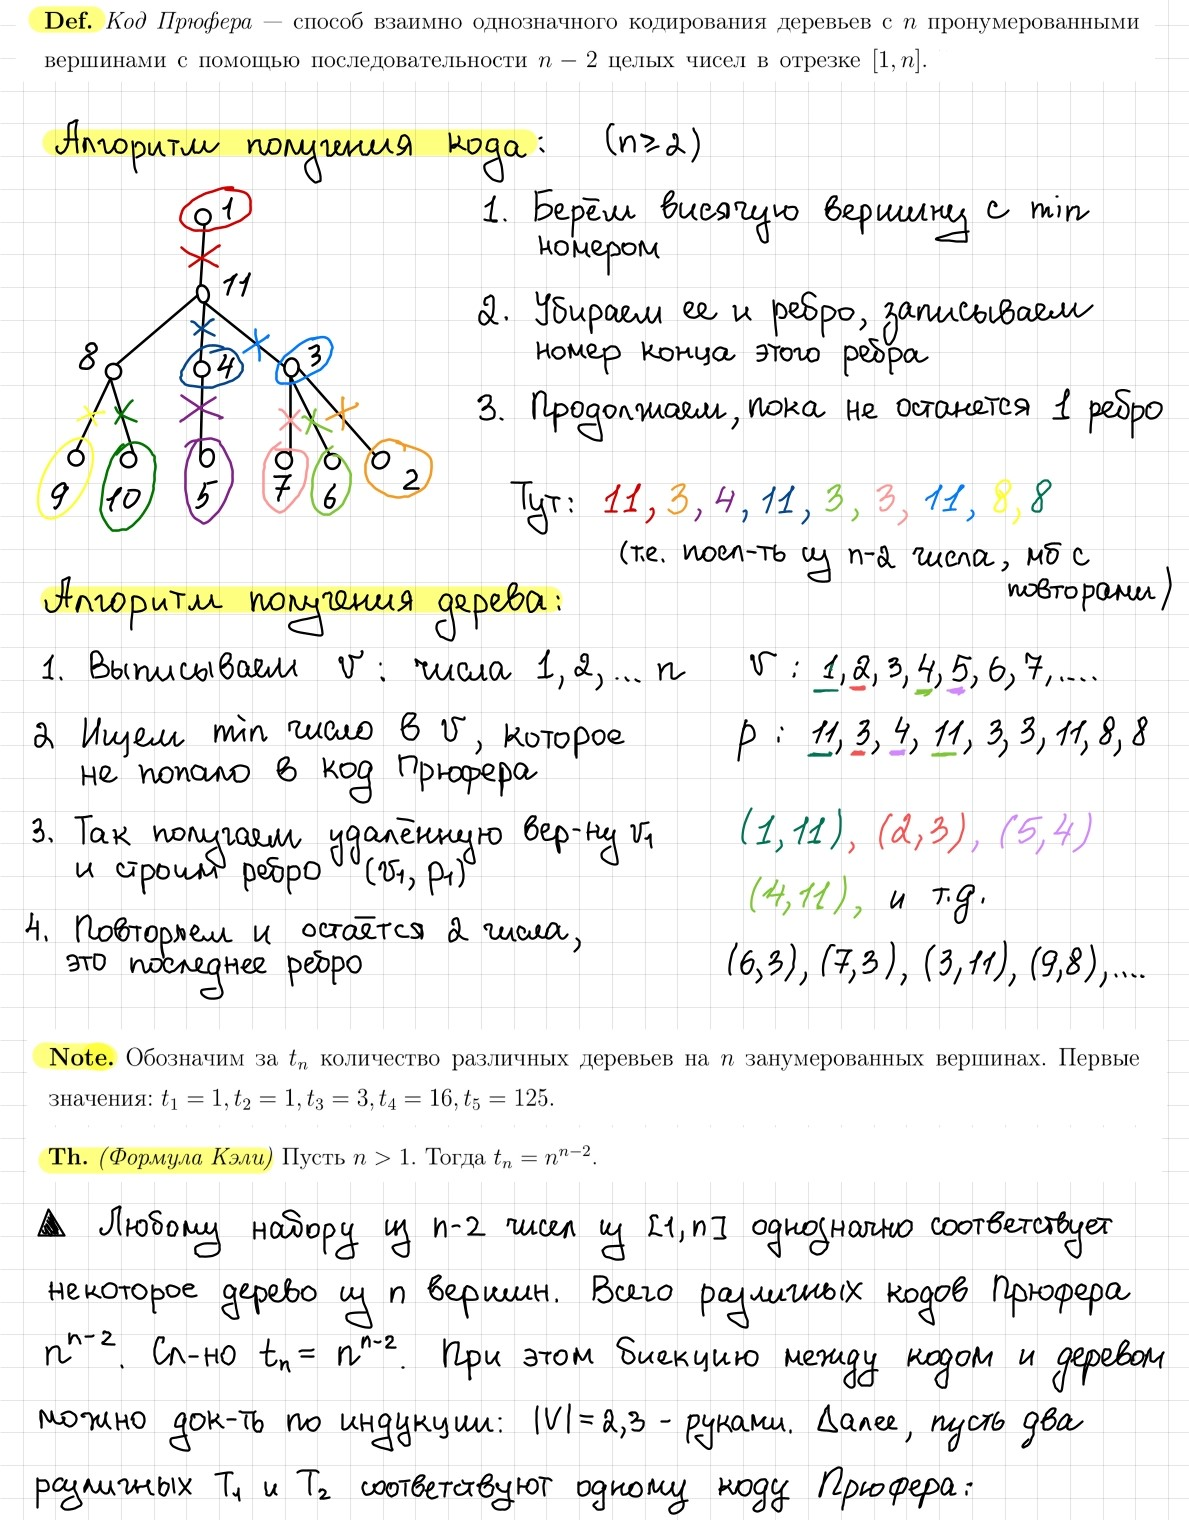
\includegraphics[width=1\linewidth]{sections/Polina/imgs/13.jpg}
\newpage 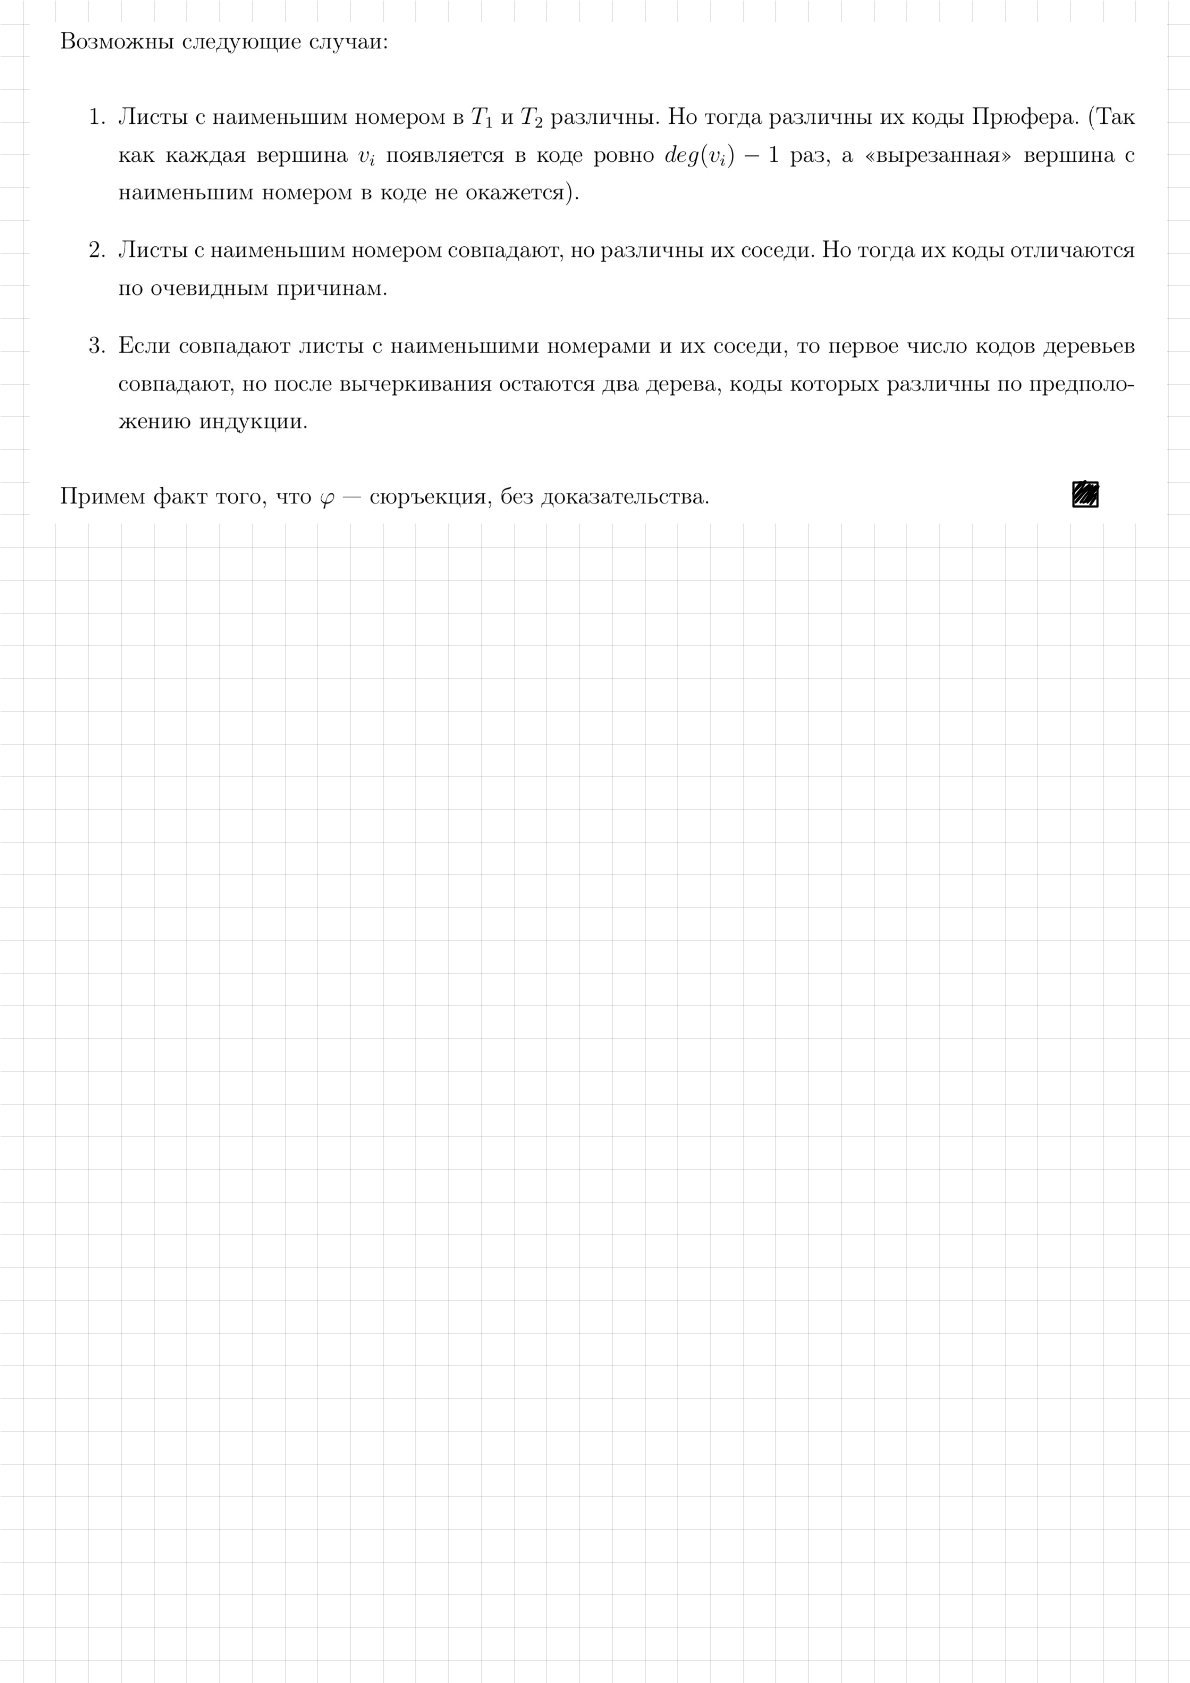
\includegraphics[width=1\linewidth]{sections/Polina/imgs/14.jpg}
\newpage{}

\subsection{3. Свойства класса автоматных языков. Замкнутость относительно булевых операций.}

\Def Полный ДКА.
Полный ДКА (ПДКА) - ДКА, для которого выполнено:
$$\forall a \in \Sigma, q \in Q \,\,\, |\Delta (q, a)| = 1$$

\Statement Для любого автоматного языка $L$ существует ПДКА $M$, такой что $L(M) = M$ (т.е. автоматы распознают одинаковое множество слов);

Метод построения ПДКА из ДКА:\\
1) строим ''стоковую'' вершину.\\
2) Добавляем из всех вершин переходы по недостающим буквам в "сток".

\begin{figure}[h]
    \hspace{-4ex} \begin{minipage}[h]{1\linewidth}
    \center{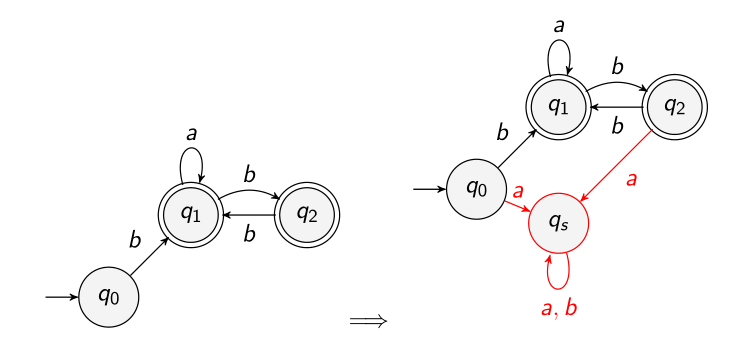
\includegraphics[width=0.6\linewidth]{1_3_1.png}}
    \end{minipage}
    \hspace{-4ex}
\end{figure}

Появятся ли новые слова? - нет, потому что, если мы попали в стоковую вершину, то не сможем ''выбраться'' из неё.

\Def Итерация Клини для языка L.
$$L^* = \cup_{k = 0}^{\infty}L^k$$

\Th Класс автоматных языков замкнут относительно\\
1. Конкатенации\\
2. Объединения\\
3. Пересечения\\
4. Итерации Клини\\
5. Дополнения

\Proof
Далее будем рассматривать только НКА с одним завершающим состоянием.
Для того чтобы после операции у итогового автомата было одно завершающее состояние, добавляем состояние и соединяем завершающие состояния с ним с помощью $\varepsilon$-переходов. (делаем новое состояние - завершающим, а старые - не завершающими)

1) Конкатенация $M_1$ и $M_2$:

Соединяем $\varepsilon$-переходами завершающее состояние $M_1$ со стартовыми состояниями $M_2$.
\begin{center}
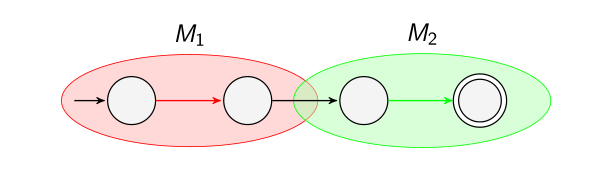
\includegraphics[width=0.45\linewidth]{1_3_2.png}
\end{center}

2) Объединение $M_1$ и $M_2$:

Добавляем стартовое состояние. Соединяем её со стартовыми состояниями $M_1$ и $M_2$ с помощью $\varepsilon$-переходов. 
\begin{center}
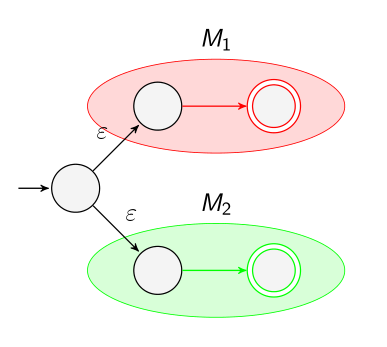
\includegraphics[width=0.25\linewidth]{1_3_3.png}
\end{center}

4) Итерации Клини над $M_1$:

Добавляем стартово-завершающее состояние. С помощью $\varepsilon$-переходов соединяем её с начальными состояниями $M_1$, а завершающее состояния $M_1$ с ней.
\begin{center}
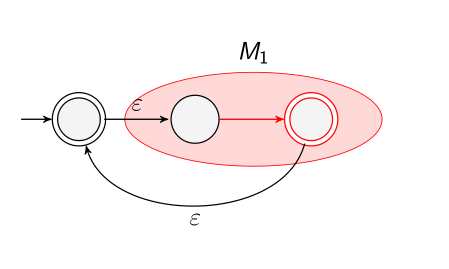
\includegraphics[width=0.32\linewidth]{1_3_4.png}
\end{center}

3) Пересечение $M_1$, $M_2$:

Строим "декартово произведение" автоматов с одно буквенными переходами.

\begin{center}
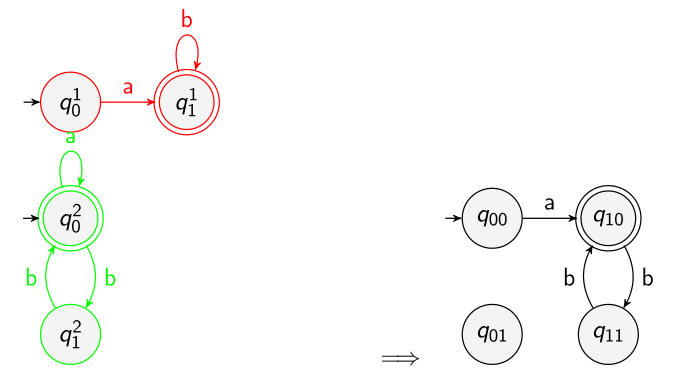
\includegraphics[width=0.55\linewidth]{1_3_5.png}
\end{center}

То есть пересечение будет состоять из состояний, каждому из которых соответствует пара чисел $(i, j)$, это номера состояний из $M_1$ и $M_2$ соответственно, которым это состояние соответствует. И между состояниями $(i_1, j_1)$ и $(i_2, j_2)$ будет проходить ребро с символом $k$, если между $i_1$ и $i_2$ проходило ребро с символом $k$ в $M_1$ и между $j_1$ и $j_2$ проходило ребро с символом $k$ в $M_2$. $(i, j)$ - стартовое состояние, если $i$ - стартовое в $M_1$, $j$ - стартовое в $M_2$. Аналогично с завершающем состоянием. 

5) Дополнение: строим ПДКА и инвертируем терминальность всех состояний.

\newpage{}

\subsection{4. Регулярные выражения. Теорема Клини о совпадении классов регулярных и автоматных языков. Регулярный автомат, алгоритм построения.}

\Vars \\
Regex (регулярное выражение) обозначим за $R$, \newline Language (язык) -- за $L$, \newline $L(R_i)$ (язык, который задается регулярным выражением $R$) -- $L_i$.

\Def Рекурсивное определение регулярного выражения.

% \begin{minipage}[r]{0.1\linewidth} 
% %\begin{flushright}
%     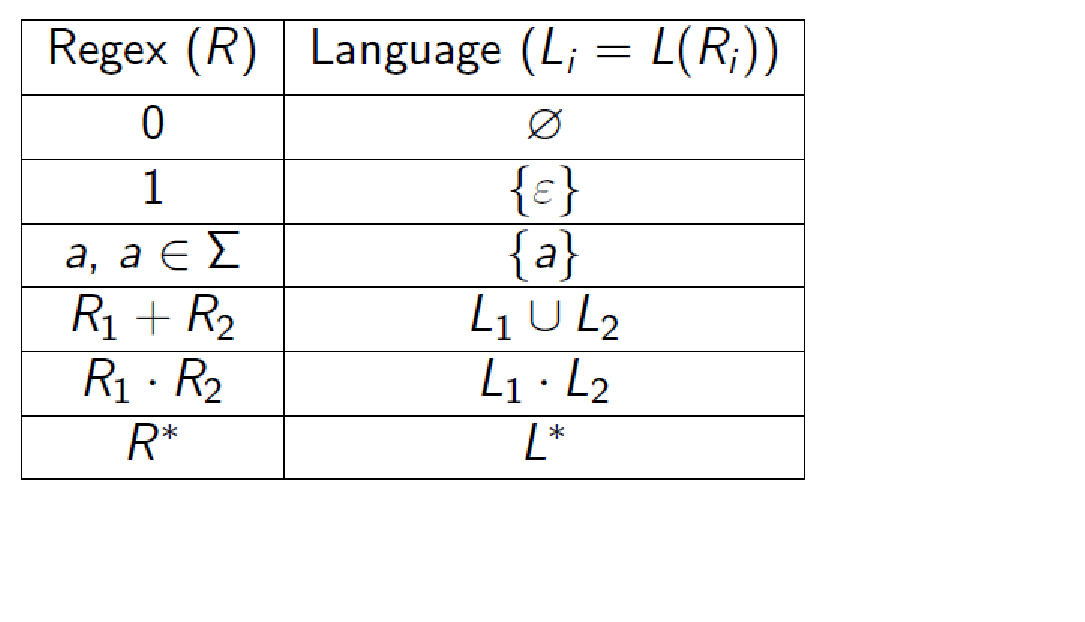
\includegraphics[width=5\linewidth]{images/1_4_1.png}
% %\end{flushright} 
% \end{minipage} 
\begin{center}
    \begin{tabular}{|c|c|}
        \hline
        $Regex (R)$ & $Language (L_i = L(R_i))$ \\
        \hline
        $0$ & $\varnothing$ \\
        $1$ & $\{ \varepsilon \}$ \\
        $a$, $a \in \Sigma$ & $\{ a \}$ \\
        $R_1 + R_2$ & $L_1 \cup L_2$ \\
        $R_1 \cdot R_2$ & $L_1 \cdot L_2$ \\
        $R^*$ & $L^*$ \\
        \hline
    \end{tabular}
\end{center}

Здесь $\varepsilon$ -- пустое слово, <<$\cdot$>> -- операция конкатенации языков (в полученном языке $L_1 \cdot L_2$ лежат слова вида $a_1a_2$, где слово $a_1$ лежит в языке $L_1$, а слово $a_2$ лежит в языке $L_2$), <<$*$>> -- звезда Клини.

Напомним определение звезды Клини: $V^* = \bigcup_{i=0}^{\infty} V^i$ 

\textbf{Приоритет операций} в регулярных выражениях (левее — приоритетнее): $* \rightarrow \cdot \rightarrow +$

\Def Язык $L$ -- регулярный, если он задается регулярным выражением.

\hspace{4ex}

\textbf{Теорема Клини:} Классы регулярных и автоматных языков совпадают.

\Proof Докажем два вложения:

\textbf{1. Регулярные $\subseteq$ Автоматные}

% \begin{figure}[h]
%     \begin{minipage}[h]{0.6\linewidth}
%     Индукция по построению выражения. 
    
%     Немного изменим утверждение -- докажем, что по регулярному выражению можно построить НКА с $1$ завершающим состоянием, который задает тот же язык.\\
    
%     \textit{База}: Построим автоматы для регулярных выражений: 0, 1, a.
%     \end{minipage}
%     \hspace{-4ex} \begin{minipage}[h]{0.5\linewidth}
%     \center{\includegraphics[width=0.6\linewidth]{images/4_base.jpg}}
%     \end{minipage}
% \end{figure}
% Регулярное выражение <<$0$>> -- автомат без завершающих состояний.

% Регулярное выражение <<$1$>> -- в автомате, состоящем из одной вершины, стартовая вершина помечается завершающим состоянием.

% Регулярное выражение <<$a$>> -- в автомате две вершины. Вершина номер $0$ стартовая, вершину номер $1$ помечаем как терминальную. Проводим ребро из $0$ в $1$, на котором пишем букву a.

Индукция по построению выражения. Немного изменим утверждение -- докажем, что по регулярному выражению можно построить НКА с $1$ завершающим состоянием, который задает тот же язык.

\textit{База}: Построим автоматы для регулярных выражений: $0, 1, a \in \Sigma$.
% %картинка%
\begin{figure}[h!]
    \centering
    \includegraphics[scale=0.27]{4_base.jpg}
\end{figure}
% \newline \center{\includegraphics[width=0.29\linewidth]{4_base.jpg}}
% \begin{minipage}[r]{1\linewidth} 
% %\begin{flushright}
%     % 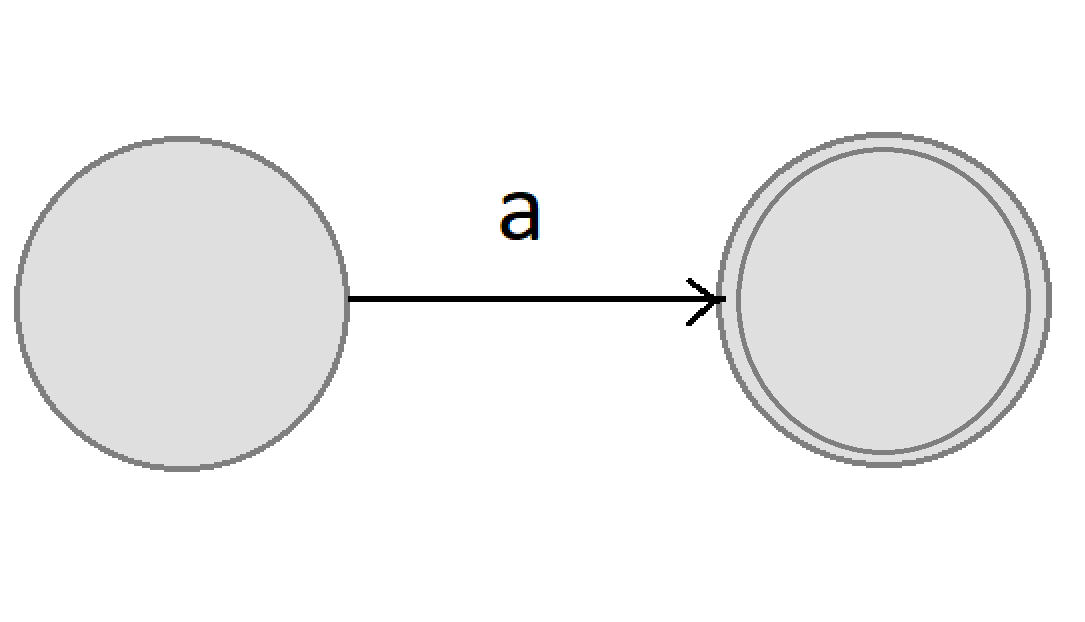
\includegraphics[width=2\linewidth]{images/1_4_2.png}
%     \center{\includegraphics[width=1\linewidth]{images/4_base.jpg}}
% %\end{flushright} 
% \end{minipage} 

\textit{Переход:}

1) $R = R_1 + R_2$. Построим автомат $A_1$ для $R_1$, для которого вершина $S_1$ -- стартовая, а вершина $F_1$ -- единственная терминальная. Для $R_2$ это будут автомат $A_2$ со стартовой вершиной $S_2$ и терминальной $F_2$.
Создадим новую вершину $S$, которая и будет стартовой в новом автомате. Из нее проведем два ребра с $\varepsilon$-переходами в $S_1$ и в $S_2$. Аналогично соединим завершающие в автоматах с новой завершающей вершиной $F$. Нетрудно доказать, что такой автомат задаст тот же язык, что и наше регулярное выражение.

2) $R = R_1 \cdot R_2$. Аналогично прошлому пункту получим автоматы для $R_1$ и $R_2$ с теми же обозначениями. Вершина $S_1$ будет стартовой в нашем новом автомате. Добавим также $\varepsilon$-переход из $F_1$ в $S_2$, уберем терминальность $F_1$.

3) $R = R_1^*$. Построим автомат $A_1$ для $R_1$ со стартовой вершиной $S_1$ и терминальной вершиной $F_1$. Создадим вершину $S$ -- новую стартовую вершину, пометим ее терминальной. Добавим из нее и из $F_1$ $\varepsilon$-переход в $S_1$.

\textbf{2. Автоматные $\subseteq$ Регулярные}

\Note{Регулярный автомат -- НКА, в котором на ребрах записаны регулярные выражения. Докажем утверждение для регулярных автоматов.}

\Note{Всякий НКА задается регулярным автоматом с 1 завершающим состоянием.}

Индукция по $|Q|$ (количеству состояний -- вершин) в регулярном автомате.

\textit{База:}

1) $|Q| = 1$. Тогда в регулярном автомате стартовое состояние является завершающим, и можно однозначно построить регулярное выражение. Такому автомату соответсвует регулярное выражение $a^*$
\newline
\begin{minipage}[r]{0.1\linewidth} 
%\begin{flushright}
    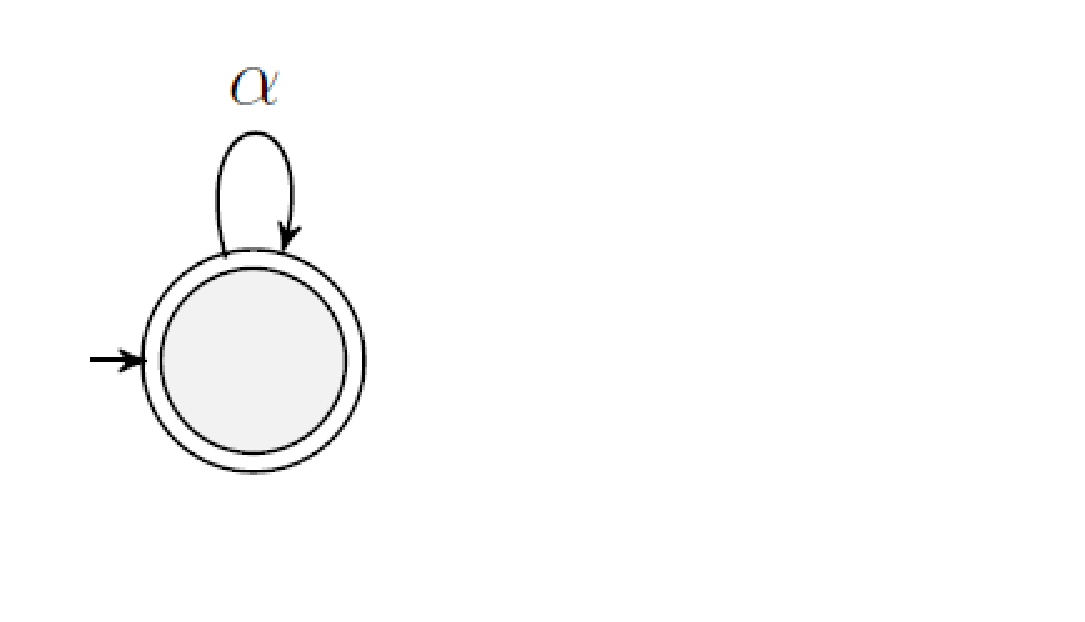
\includegraphics[width=4\linewidth]{images/1_4_3.png}
%\end{flushright} 
\end{minipage} 

2) $|Q| = 2$. Cтартовое состояние и завершающее состояние различны, и можно тоже однозначно построить регулярное выражение. Такому автомату соответсвует регулярное выражение $\alpha^*\beta(\gamma + \delta \alpha^* \beta)^*$
\newline
\begin{minipage}[r]{0.1\linewidth} 
%\begin{flushright}
    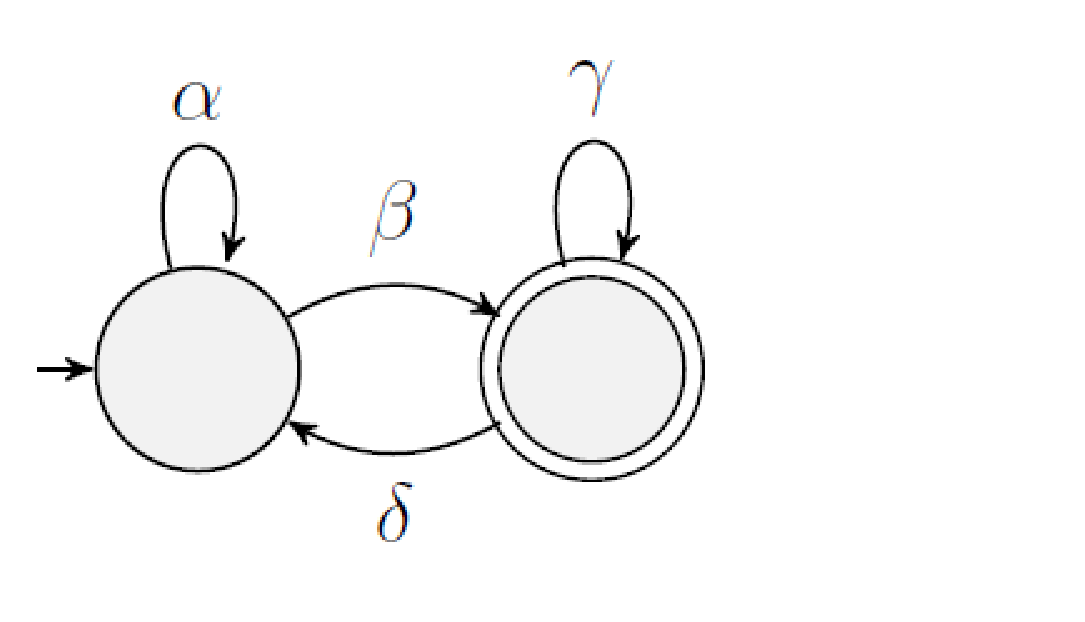
\includegraphics[width=4\linewidth]{images/1_4_4.png}
%\end{flushright} 
\end{minipage} 

Для случая, когда завершающее состояние -- это начальная вершина, регулярное выражение будет $(\gamma + \delta \alpha^* \beta)^*$.

\textit{Переход:}
\Note{Есть нестартовая и незавершающая вершина!}

1) Удаляем кратные ребра:
\begin{minipage}[r]{0.2\linewidth} 
%\begin{flushright}
    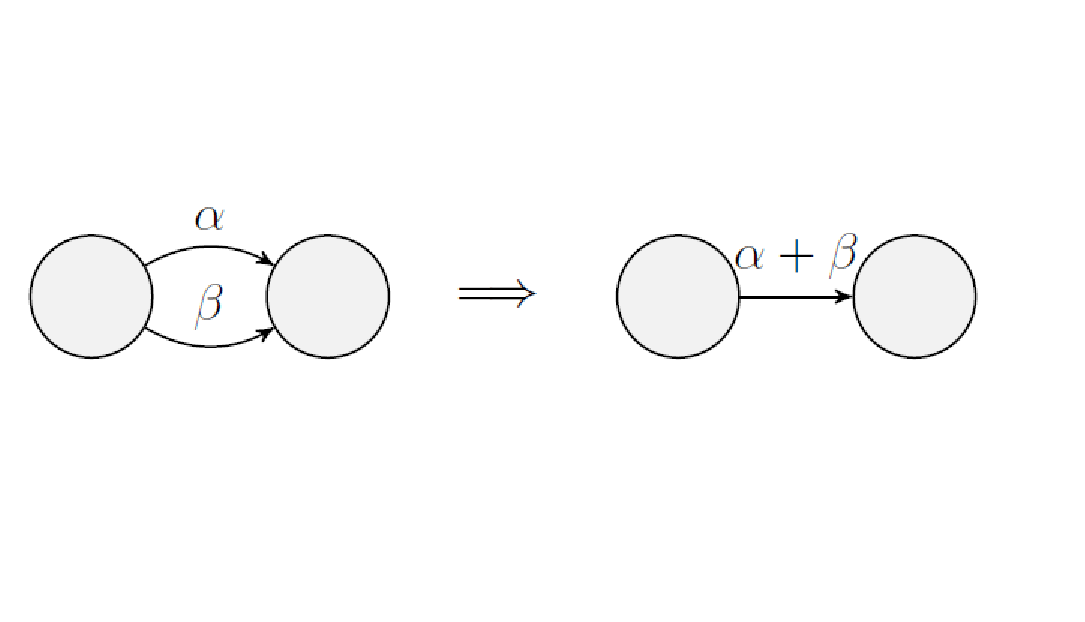
\includegraphics[width=2.5\linewidth]{images/1_4_5.png}
%\end{flushright} 
\end{minipage} 

Кратные ребра означают, что мы можем выбрать, какой символ будем использовать. Именно этот смысл и несет в себе операция <<$+$>>.

2) Добавляем циклы на себя:
\begin{minipage}[r]{0.1\linewidth} 
%\begin{flushright}
    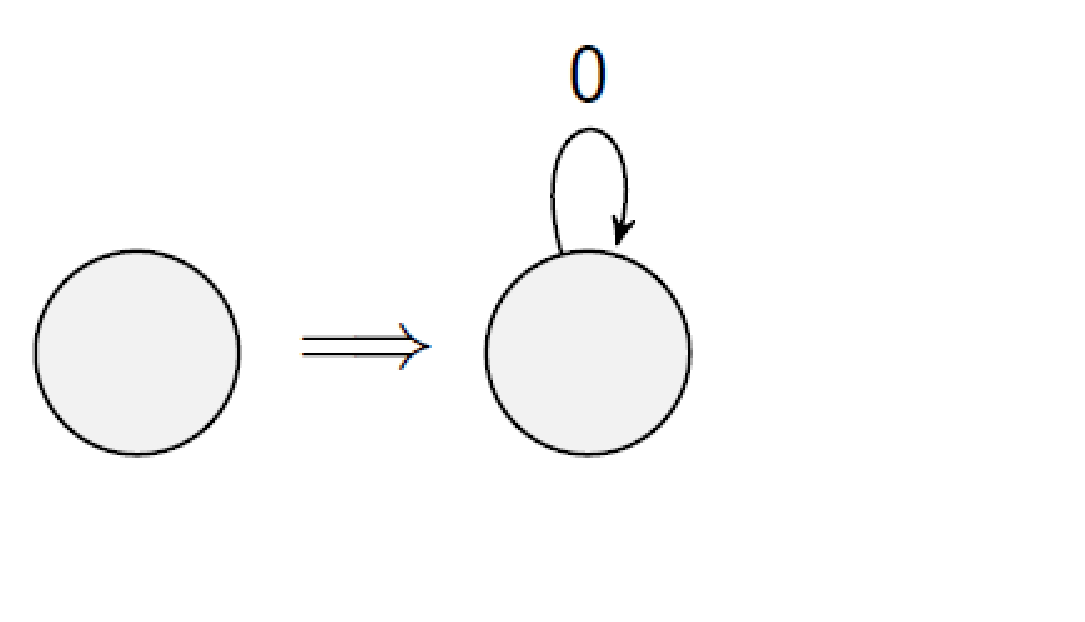
\includegraphics[width=3.5\linewidth]{images/1_4_6.png}
%\end{flushright} 
\end{minipage} 

3) Удаляем нестартовое и незавершающее состояние:

\begin{minipage}[r]{0.1\linewidth} 
%\begin{flushright}
    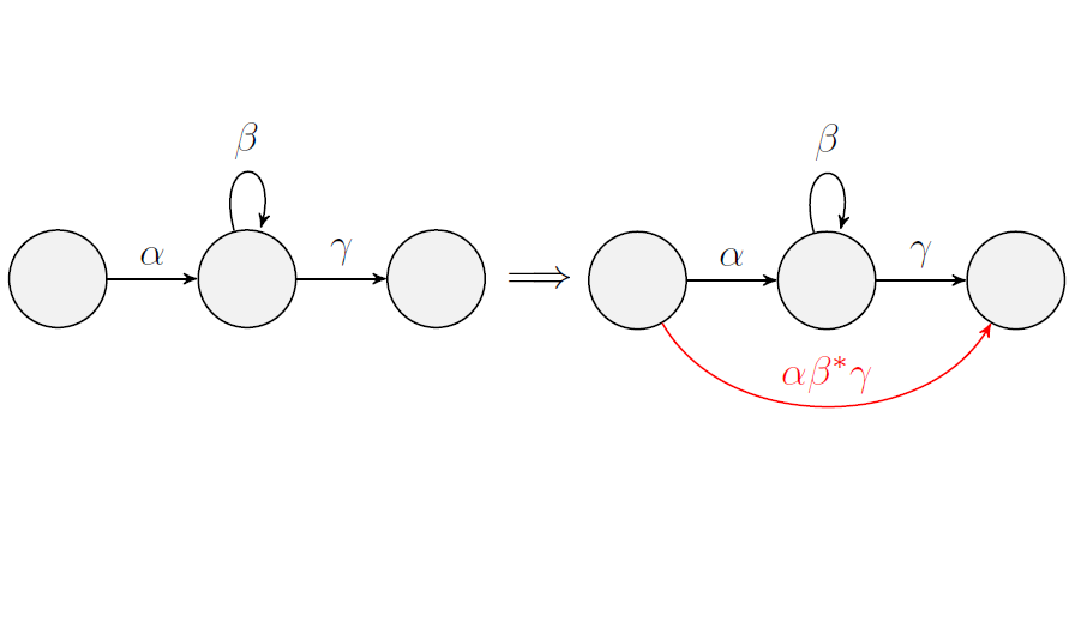
\includegraphics[width=5.5\linewidth]{images/1_4_7.png}
%\end{flushright} 
\end{minipage} 
\newline Теперь у нас на одно сотояние стало меньше, т.е. мы можем воспользоваться утверждением индукции.
\EndProof
\newpage{}

\subsection{5. Минимальный ДКА, его существование.}

\textbf{Мотивировка:} может быть много состояний. А еще не очень понятно, как сравнивать два автомата на эквивалентность. Вернее, если проверять <<в лоб>>, будет долго. Один из способов решить эти проблемы -- минимизация автомата.\\

Пусть $L \subset \Sigma^*$ -- автоматный язык, $M$ -- ПДКА для $L$.

\Def Минимальный ПДКА $M$, распознающий язык $L$, если $M$ -- минимальный по количеству состояний.

\hspace{4ex}

\Def Определим отношение эквивалентности $\sim_L$ на $\Sigma^*:$
$$u \sim_L v \Longleftrightarrow \forall w \in \Sigma^* \,\,(uw \in L \Longleftrightarrow vw \in L)$$

Определение корректно (рефлексивность, симметричность и транзитивность очевидны).

\textit{Множество классов эквивалентности в этом случае:} 
$\Sigma^* /_{\sim_L}:= \{\{u \arrowvert u \sim_L v\} \,\,\arrowvert\,\, v \in \Sigma^*\}$

\Def Определим отношение эквивалентности $\sim_M$ на $Q:$
$$q_1 \sim_M q_2 \Longleftrightarrow \forall w \in \Sigma^*\,\,(\Delta(q_1, w) \in F \Longleftrightarrow \Delta(q_2, w) \in F)$$

Если $q_1 \sim_M q_2$, то состояния можно объединить.

\textit{Напоминание:} Множество вершин, достижимых из $q$ по $w$ -- $\Delta (q, w) = \{ q' | \langle q, w \rangle \vdash \langle q', \varepsilon \rangle \}$..\\

% \hspace{4ex} 
\textbf{Лемма}
Пусть $L_q := \{w \,\arrowvert\, \Delta(q_0, w) = q\}$. Тогда каждый класс эквивалентности в нашем фактор-множестве являетеся объединением классов в $L_q$.

\Proof
Возьмем слово $u \in [u] \in \Sigma^*/_{\sim_L}$, где $[u]$ -- это класс эквивалентности для $u$. Рассмотрим путь по $u$ из $q_0$, а именно,  $q_u = \Delta(q_0, u)$. Для любого слова $w \in [u]$, $q_w = \Delta \brackets{q_0, w}$. Тогда $[u] = \bigcup \limits_{q_w, w \in [u]} L_{q_w}$. Далее докажем, почему это так.
% Из последнего очевидно, что $u \in L_{q_u}$. 

Пусть $v \in [u] \,\Longrightarrow\, v \sim_L u \,\Longrightarrow\, q_v = \Delta \brackets{q_0, v} \,\Longrightarrow\, v \in L_{q_v}$. Тогда $v \in \bigcup \limits_{q_w, w \in [u]} L_{q_w}$.

Пусть $v \in \bigcup \limits_{q_w, w \in [u]} L_{q_w}$. Тогда существует состояние $q_z$, $z \in [u]$, что $v \in L_{q_z} = \{ w | \Delta \brackets{q_0, w} = q_z \}$.
\begin{center}
    $z \in [u] \Longrightarrow z \sim_L u \stackrel{def}{\Longrightarrow} \; \forall w \in \Sigma^* \; \brackets{zw \in L \Longleftrightarrow uw \in L}$
    \begin{equation*}
        \left.
          \begin{array}{ccc}
            v \in L_{q_z} \Longrightarrow & \Delta \brackets{q_0, v} & = q_z \\
            & \Delta \brackets{q_0, z} & = q_z \\
          \end{array}
        \right\} \quad
    \Longrightarrow \quad v \sim_L z \text{ так как $\forall w \in \Sigma^*$ $\Delta \brackets{q_0, vw} \stackrel{(*)}{=} \Delta \brackets{q_0, zw}$}
    \end{equation*}
\end{center}

$\brackets{*}$: $\Delta \brackets{q_0, vw} = \Delta \brackets{\Delta(q_0, v), w} = \Delta \brackets{q_z, w} = \Delta \brackets{\Delta(q_0, z), w} = \Delta \brackets{q_0, zw}$

Так как $v \sim_L z$, $z \in [u]$, то $v \in [u]$. Значит, $[u] = \bigcup \limits_{q_w, w \in [u]} L_{q_w}$, и каждый класс эквивалентности из $\Sigma^* /_{\sim_L}$ — объединение классов в $L_q$. \quad \EndProof

% И так для любого элемента $w \in [u] \hookrightarrow w \in L_{q_w}$. Поэтому \[ [u] \subset \bigcup_{q_w, w \in [u]} L_{q_w}.\]

% Докажем теперь обратное включение. Возьмем $v \in L_{q_w}$. Для него верно $q_v = \Delta(q_0, v) = q_w$. Докажем, что тогда $v \in [w]$ ($[u] = [w]$).

% Возьмем произвольное $m \in \Sigma^*$. Заметим, что тогда верно $vm \in L \Longleftrightarrow wm \in L$, ведь слово $w$ читается из состояния $q_v$ и приводит в завершающее тогда и только тогда, когда то же самое верно и для $q_w$ (просто в силу того, что $q_v = q_w$).


\textbf{Следствие}
$\arrowvert \Sigma^*/_{\sim_L} \arrowvert \leq \arrowvert Q \arrowvert$\\

\textit{Теперь перейдем к минимальному ПДКА, а именно докажем его существование (тут) и единственность с точностью до изоморфизма (билет 6).}\\

\textbf{Лемма} Для любого автоматного языка $L$ существует ПДКА $M'$ такой, что все состояния в $M'$ попарно неэквивалентны.

Что необходимо доказать?\\
1) Переходы и завершающие состояния согласованы\\
2) Распознаваемые языки совпадают\\
3) Состояния попарно неэквивалентны

\Proof Рассмотрим автомат над классами эквивалентности $\sim_M$. Класс эквивалентности $q$ обозначим за $[q]$. $M' = \langle Q /_{\sim_M}, \Sigma, \Delta', [q_0], F' \rangle$, где:

\begin{center}
    $\Delta' = \{ \langle [q_1], a \rangle \rightarrow [q_2] \;|\; \exists \langle q_1, a \rangle \rightarrow q_2 \in \Delta \}$
    
    $F' = \{ [q_f] \;|\; q_f \in F \}$
\end{center}

1) Проверим, что множества $\Delta'$, $F'$ заданы корректно.

Для $\Delta'$: Пусть $q_1 \sim_m q_1'$, и существует $a$ такое, что $\Delta \brackets{q_1, a} \nsim_m \Delta \brackets{q_1', a}$.
\begin{center}
    $q_1 \sim_M q_1' \stackrel{def}{\Longrightarrow} (\forall w \in \Sigma^* \;\;\Delta \brackets{q, w} \in F \Longleftrightarrow \Delta \brackets{q_1', w} \in F)$
    
    $w = au \Longrightarrow (\forall u \in \Sigma^* \;\; \Delta \brackets{q_1, au} \in F \Longleftrightarrow \Delta \brackets{q_1', au} \in F)$
\end{center}

Далее обозначим $\Delta \brackets{q_1, a} = q_2$, a $\Delta \brackets{q_1', a} = q_2'$.
\begin{center}
    $\Delta \brackets{q_1, au} = \Delta \brackets{\Delta(q_1, a), u} = \Delta \brackets{q_2, u}$
    
    $\Delta \brackets{q_1', au} = \Delta \brackets{q_2', u}$
    
    $(\Delta \brackets{q_2, u} \in F \Longleftrightarrow \Delta \brackets{q_2', u} \in F)\; \Longrightarrow q_2 \sim_m q_2'$.
\end{center}

Приходим к противоречию.

Для $F'$:
\begin{center}
    $q_1 \in F$, $q_2 \sim_M q_1 \overset{w = \varepsilon}{\Longrightarrow} (\Delta \brackets{q_1, \varepsilon} \in F \Longleftrightarrow \Delta \brackets{q_2, \varepsilon} \in F)$
    
    Значит, $q_1 \in F \Longleftrightarrow q_2 \in F$
\end{center}

2) Теперь покажем, что $L \brackets{M} = L \brackets{M'}$. 

Для этого нужно показать, что $w \in L \brackets{M} \Longleftrightarrow \Delta \brackets{q_0, w} \in F \stackrel{?}{\Longleftrightarrow} \Delta \brackets{[q_0], w} \in F'$.

Докажем утверждение: $\forall u: \Delta \brackets{q_0, u} = q_1 \Longleftrightarrow \Delta \brackets{[q_0], u} = [q_1]$.

Индукция по длине слова $u$.

\textbf{База.} $|u| = 0 \Longrightarrow u = \varepsilon$. Тогда $\Delta \brackets{q_0, \varepsilon} = q_0$, $\Delta \brackets{[q_0], \varepsilon} = [q_0]$.

\textbf{Переход.} Пусть $u = va$, $v \in \Sigma^*$, $a \in \Sigma$.

\begin{center}
    $\Delta \brackets{q_0, va} = q_1 \Longrightarrow \exists q_2\; \Delta \brackets{q_0, v} = q_2, \;\Delta \brackets{q_2, a} = q_1$
\end{center}

По предположению индукции, $\Delta \brackets{[q_0], u} = [q_2]$, $\Delta \brackets{[q_2], a} = [q_1]$, так как переход $\langle q_2, a \rangle \rightarrow q_1 \in \Delta$ тогда и только тогда, когда $\langle [q_2], a \rangle \rightarrow [q_1] \in \Delta'$. По транзитивности, $\Delta \brackets{[q_0], ua} = [q_1]$.

3) Теперь покажем, что состояния попарно неэквивалентны. В автомате, построенном на классах эквивалентности состояний никакие два состояния не эквивалентны, потому что тогда бы они лежали в одном классе, т.е. были бы одним состоянием.

Пусть $[q_1] \sim_{M'} [q_2]$. Тогда $\forall w : \Delta_{M'} \brackets{[q_1], w} \in F' \Longleftrightarrow \Delta_{M'} \brackets{[q_2], w} \in F'$ по определению. 

\begin{center}
    $[q_{1f}] = \Delta_{M'} \brackets{[q_1], w} \in F'$
    
    $[q_{2f}] = \Delta_{M'} \brackets{[q_2], w} \in F'$
    
    $\exists q_{1f} \in F : \Delta_M \brackets{q_1, w} = q_{1f} \in F \Longleftrightarrow \exists q_{2f} \in F : \Delta_M \brackets{q_2, w} = q_{2f} \in F$
    
    $q_1 \sim_{M} q_2 \Longrightarrow [q_1] = [q_2]$
\end{center}
\begin{flushright}
  \EndProof
\end{flushright} 


\Th $M$ — минимальный ПДКА, распознающий язык $L$, тогда и только тогда, когда любые два состояния попарно неэквивалентны и все состояния достижимы из стартового.

\textit{Теперь запишем более формально:}

\begin{center}
    $M$ — минимальный ПДКА $\Longleftrightarrow \begin{cases} \forall q_1, q_2 \in Q \ q_1 \nsim q_2 \\ \forall q \in Q \ \exists w \in \Sigma^* : \ \langle q_0, w \rangle \vdash \langle q, \varepsilon \rangle \end{cases}$
\end{center}

\Proof

$\Longrightarrow$ Если $q_1 \sim_M q_2$, то $[q_1] = [q_2]$, и их можно объединить в одно состояние, значит, $M$ не был бы минимальным, и тогда из минимальности следует, что $q_1 \nsim_M q_2$. Если среди состояний есть недостижимые, то если их удалить, то множество принимаемых слов не изменится.

$\Longleftarrow$ По следствию из леммы о $L_q$: $|\Sigma^* /_{\sim_L}| \leqslant |Q|$. Рассмотрим $w_1$, $w_2$ такие, что $\Delta \brackets{q_0, w_1} \neq \Delta \brackets{q_0, w_2}$. Введём обозначения:

\begin{center}
    $\Delta \brackets{q_0, w_1} = q_1$
    
    $\Delta \brackets{q_0, w_2} = q_2$
\end{center}

Неэквивалентность состояний $q_1$, $q_2$ означает, что существует слово $w$, что б.о.о:

\begin{center}
    $\Delta \brackets{q_1, w} = \Delta \brackets{q_0, w_1 w} \in F \Longleftrightarrow w_1 w \in L$
    
    $\Delta \brackets{q_2, w} = \Delta \brackets{q_0, w_2 w} \notin F \Longleftrightarrow w_2 w \notin L$
    
    Следовательно, получили что $w_1 \nsim_L w_2$
\end{center}

Тогда для автомата $M$ со множеством состояний $Q'$ выполняется, что $|\Sigma^* /_{\sim_L}| \geqslant |Q'|$, но тогда $|Q| \geqslant |\Sigma^* /_{\sim_L}| \geqslant |Q'|$, и $M$ — минимальный. \quad \EndProof
\newpage{}

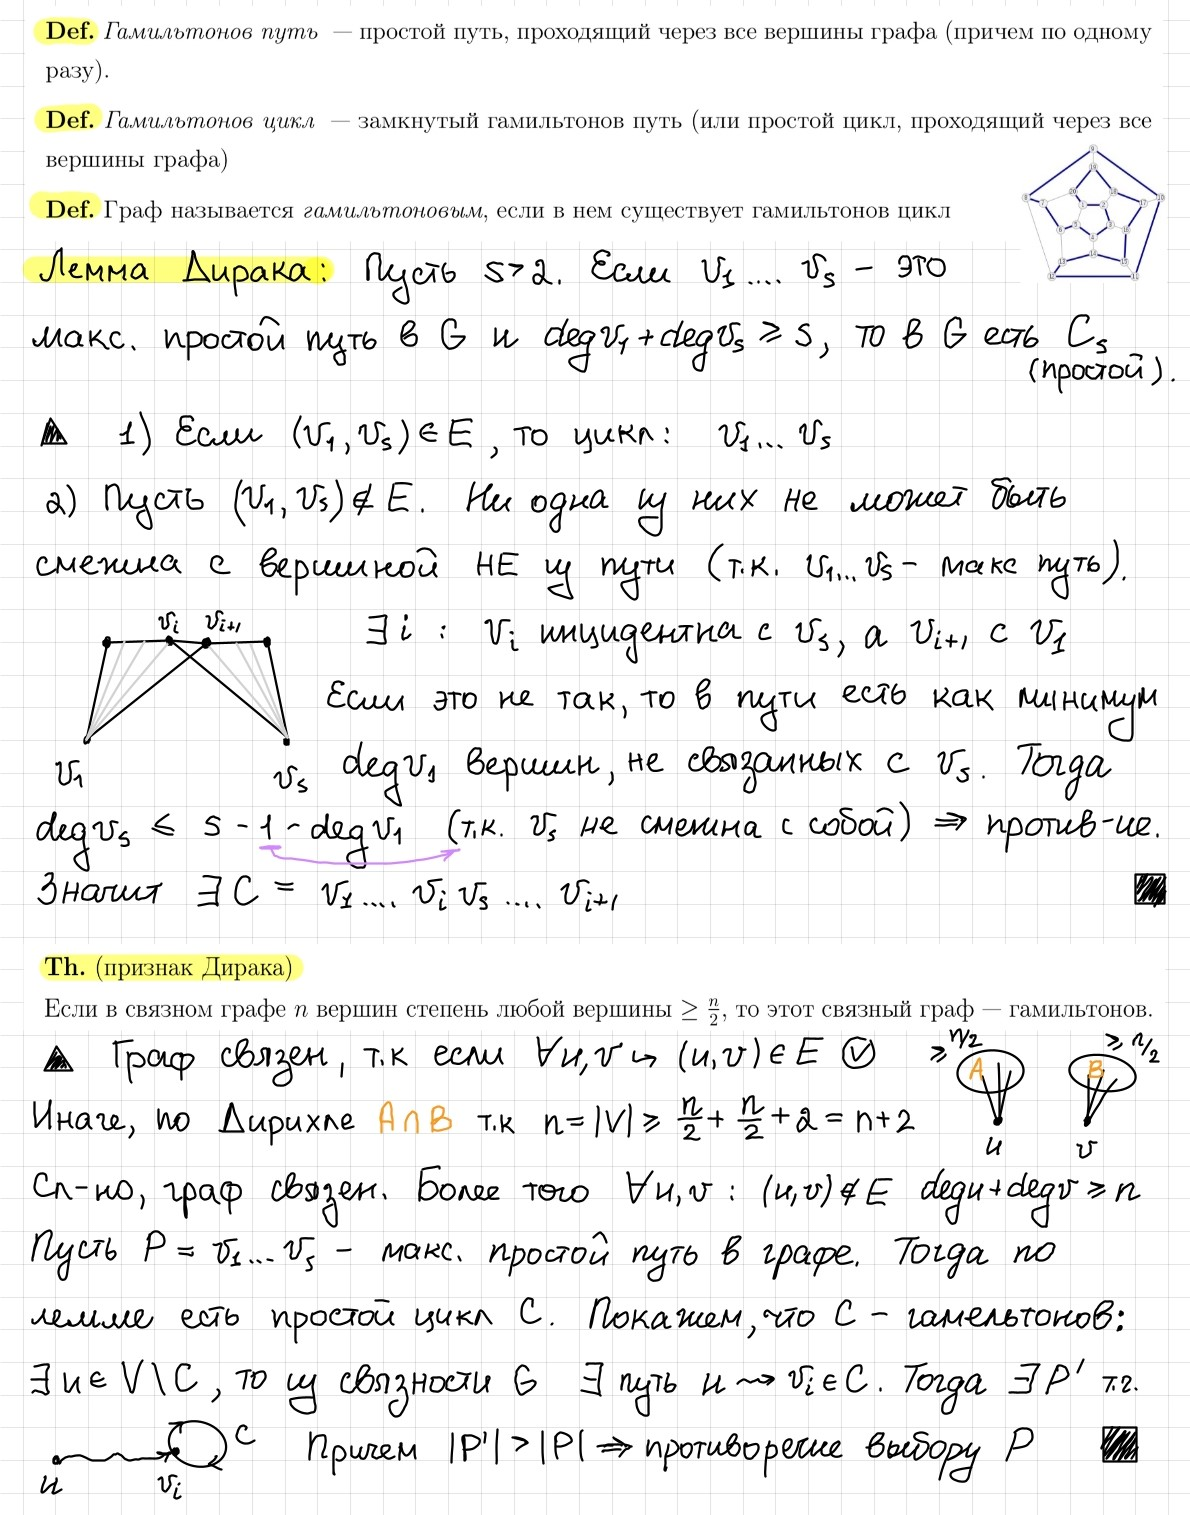
\includegraphics[width=1\linewidth]{sections/Polina/imgs/25.jpg}
\newpage{}

\setcounter{section}{6}

\section{Понятия образа и прообраза множества при соответствии. Критерий равенства образа пересечения и пересечения образов. Аналогичные критерии с объединением и разностью.} 
\textbf{Соответствие} между множествами A и B - произвольное подмножество декартова произведения $F \subset A \times B$. Обозначение: $F: A \to B$; иногда, чтобы подчеркнуть, что одному элементу из A может соответствовать несколько элементов из B, пишут: $F:A\rightrightarrows B$. 
\\
\par
Пусть $F: A \to B$ - соответствие, $S \subset A$, $T \subset B$. Тогда \textbf{образ} множества S - множество всех элементов B, соответствующих какому-то элементу S. Формально: $F(S) = \bigcup_{s \in S} F(s) \subset B $. \textbf{Прообраз} множества Т - множество элементов А, которым соответсвует хотя бы один элемент Т. Формально: $F^{-1}(T) = \left\{ a: F(a) \cap T \neq \varnothing \right\}$ 
\\
\par
\emph{ Образ пересечения любых двух множеств равняется пересечению образов тех же множеств $\iff$ соответствие инъективно. } 
\\
$\blacktriangle$
Пусть соответствие не инъективно. Тогда найдутся такие $a_1$ и $a_2$, что $F(a_1)$ и $F(a_2)$ пересекаются. Тогда $F(\left\{a_1\right\} \cap \left\{a_1\right\}) = F(\varnothing) = \varnothing$, но $F(\left\{a_1\right\}) \cap F(\left\{a_2\right\}) = F(a_1) \cap F(a_2)$ не пуст по предположению. Значит, образ пересечения множеств $\left\{ a_1\right\}$ и $\left\{ a_2\right\}$ не равен пересечению образов. \par
Теперь пусть соответствие инъективно. Рассмотрим произвольные подмножества S и Q множества А. Докажем, что $F(S \cap Q) = F(S) \cap F(Q)$. Для этого докажем включение в обе стороны. Вначале пусть $y \in F(S \cap Q)$. Это значит, что $y \in F(x)$ для некоторого $x \in S \cap Q$. Тогда $x \in S$ и $x \in Q$. А раз $y \in F(x)$, то $y \in F(S)$ и $y \in F(Q)$. Значит, $y \in F(S) \cap F(Q)$. (Это включение верно для всех соответствий). \par
Теперь пусть $y \in F(S) \cap F(Q)$. Значит, $y \in F(x_1)$ для некоторого $x_1 \in S$ и $y \in F(x_2)$ для некоторого $x_2 \in Q$. Но при $x_1 \neq x_2$ в силу инъективности множества $F(x_1)$ и $F(x_2)$ не пересекаются. А их пересечение содержит хотя бы y. Значит, $x_1 = x_2 = x$, и $x \in S \cap Q$. А так как $y \in F(x)$, то получаем $y \in F(S \cap Q)$.
$\blacksquare$ \\
\par
\emph{ Образ объединения любых двух множеств равняется объединению образов тех же множеств - выполняется для любых соответствий. } \\
$\blacktriangle$
1) $\left.
  \begin{array}{ccc}
    A \subseteq A \cup B \Rightarrow F(A) \subseteq F(A \cup B) \\
    B \subseteq A \cup B \Rightarrow F(B) \subseteq F(A \cup B) \\
  \end{array}
\right\} \Rightarrow F(A) \cup F(B) \subseteq F(A \cup B) $ \\
2) $y \in F(A \cup B) \Rightarrow \exists x \in A \cup B: y = F(x) \Rightarrow \exists x \in A \cup x \in B: y = F(x) \Rightarrow$ \\
$\Rightarrow y \in F(A) \cup y \in F(B) \Rightarrow y \in F(A) \cup F(B) \Rightarrow  F(A \cup B) \subseteq F(A) \cup F(B) $; \\
Из пунктов 1 и 2 следует, что $F(A \cup B) = F(A) \cup F(B) $
$\blacksquare$ \\
\par
\emph{ Образ разности любых двух множеств равняется разности образов тех же множеств $\iff$ соответствие инъективно. } \\
Доказательство аналогично доказательству для пересечения.
\newpage{}

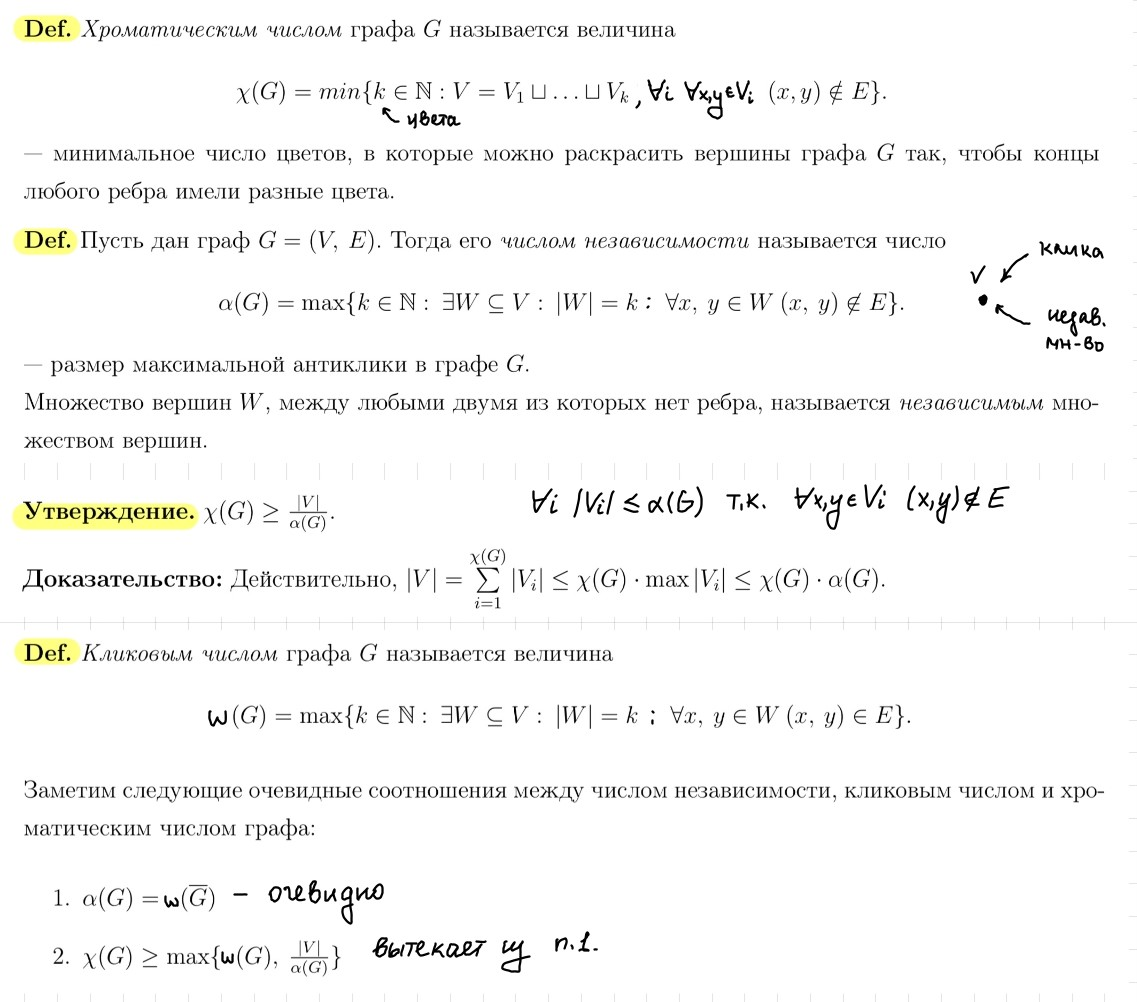
\includegraphics[width=1\linewidth]{sections/Polina/imgs/5.jpg}
\newpage{}

\setcounter{section}{8}
\section{Проверка правильности скобочной последовательности с несколькими типами скобок.}
\par \textbf{Определение}: \textit{Правильные скобочные последовательности с несколькими типами скобок} (рассмотрим с двумя)
\begin{enumerate}
    \item $\varepsilon$ (пустое слово) - ПСП
    \item $S$ - ПСП $\Rightarrow (S), [S]$ - ПСП
    \item $S_1, S_2$ - ПСП $\Rightarrow S_1 S_2$ - ПСП 
\end{enumerate}
\par \textbf{Задача:} Проверить, является ли последовательность из нескольких типов скобок правильной скобочной последовательностью
\par \textbf{Решение:} Храним стек незакрытых открывающих скобок
\lstinputlisting[language=C++,
emph={int,char,double,float,unsigned},
emphstyle={\color{blue}}
]{code/9_psp.cpp}
\par \textbf{Утверждение:} Данный алгоритм корректен, то есть ПСП $\Leftrightarrow$ алгоритм вывел true
\begin{itemize}
    \item[$\blacktriangle \Rightarrow$] Индукция по построению \begin{enumerate}
    \item База: $\varepsilon$ - обработается корректно
    \item $T=(u)$, $u$ - ПСП. По предположению индукции, всё $u$ удалится из стека к моменту прихода закрывающей скобки (можно считать, что стек начинается после первой скобки, она никак не влияет на применение алгоритма к $u$), а внешние скобки обработаются корректно (аналогично для других типов скобок)
    \item $T=T_1 T_2; T_1, T_2$ - ПСП. По предположению индукции, после того как считается $T_1$ стек опустошится $\Rightarrow$ после $T_2$ - тоже $\Rightarrow$ алгоритм сработает корректно $\blacksquare$
    \end{enumerate}
    \item[$\Leftarrow$] Доказываем индукцией по количеству действий, "обращая" предыдущий пункт.
    \par Рассмотрим скобочную последовательность, на которую алгоритм выдаёт true. Алгоритм сопоставил каждой открывающейся скобке одного типа закрывающуюся скобку того же типа. Причём они обязательно идут в правильном порядке. 
\parДля доказательства факта используем индукцию.
Рассмотрим пары соответсвующих скобок в порядке закрытия пары:
\begin{enumerate}
    \item База: Если между парой скобок нет других скобок, то последовательность от одной скобки до другой - правильная.
    \item Шаг: Если между парой скобок (назовём их $a$ и $b$ соответственно) есть непустая подстрока, то все скобки из подстроки уже были рассмотрены индукцией, так как открывающиеся скобки в подстроке были позже, чем $a$ добавлены в стек и по правилу стека должны были раньше из него выйти, а значит они уже были рассмотрены индукцией. Аналогично с закрывающимеся скобками из подстроки - они идут раньше, чем $b$, следовательно, по правилу стека им ставили в соответствие открывающиеся скобки, которые были добавленны позже $a$. (окрывающаяся скобка не могла быть добавленны раньше $a$, потому что $a$ перегородила бы ей выход.) По предположению индукции получаем, что подстрока состоит из одной или нескольких ПСП $\Rightarrow$ сама подстрока ПСП. $\Rightarrow$ Подпоследовательность от $a$ до $b$ - правильная. $\blacksquare$
\end{enumerate}
\end{itemize} 
\newpage{} 
    
\mysection{3}{3. Парсеры}
    \section{Асимптотические обозначения: $O, \Omega, \Theta$. Независимость от стартового индекса. Мастер-теорема (б/д).}
\par \textbf{Определение:} Пусть $f,g: \; \mathbb{N} \rightarrow \mathbb{N}$. Тогда $f=O(g)$, если существует $c, N$, такие что $\forall n \in N \; \hookrightarrow n \geqslant N \Rightarrow f(n) \leqslant c \cdot g(n)$.
\par \textbf{Определение:} Пусть $f,g: \; \mathbb{N} \rightarrow \mathbb{N}$. Тогда $f=\Omega(g)$, если существует $c, N$, такие что $\forall n \in N \; \hookrightarrow n \geqslant N \Rightarrow f(n) \geqslant c \cdot g(n)$.
\par \textbf{Замечание:} $f = \Omega(g) \Leftrightarrow g = O(f)$
\par \textbf{Определение:} Пусть $f,g: \; \mathbb{N} \rightarrow \mathbb{N}$. Тогда $f=\Theta(g)$, если существует $c_1,c_2, N$, такие что $\forall n \in N \; \hookrightarrow \\ n \geqslant N \Rightarrow c_1 \cdot g(n) \leqslant f(n) \leqslant c_2 \cdot g(n)$.
\par \textbf{Замечание:} $f = \Theta(g) \Leftrightarrow f = O(g)$ и $f = \Omega(g)$
\par \textbf{Утверждение:} $f = O(g) \Leftrightarrow \exists c: \forall n \in \mathbb{N} \hookrightarrow f(n) \leqslant c \cdot g(n)$ 
\par \begin{itemize}
    \item[$\blacktriangle \Leftarrow$] Очевидно, достаточно положить $N=1$
    \item[$\Rightarrow$] Пусть $\forall n \geqslant N \hookrightarrow f(n) \leqslant c \cdot g(n)$. Определим $c'=\max \{c, \frac{f(1)}{g(1)}, \ldots, \frac{f(N)}{g(N)}\}$ ($g$ не обращается в 0 так как результат натуральный). Тогда \begin{enumerate}
        \item $n \geqslant N \Rightarrow f(n) \leqslant c \cdot g(n) \leqslant c' \cdot g(n)$
        \item $n < N \Rightarrow c' \geqslant \frac{f(n)}{g(n)} \Rightarrow f(n) \leqslant c' \cdot g(n) \; \blacksquare$
    \end{enumerate}
\end{itemize}
\par Для $\Omega$ и $\Theta$ справедливы аналогичные утверждения.
\par \textbf{Мастер-теорема (с лекции):} Пусть $T: \mathbb{N} \rightarrow \mathbb{N}$ с условием $T(n)=a \cdot T(\frac{n}{b})+f(n)$, $a=const, a \geqslant 1; \\ b=const, b \geqslant 1, f: \mathbb{N} \rightarrow \mathbb{N}$. Тогда \begin{enumerate}
    \item Если $\exists \varepsilon > 0$, такое что $f(n)=O(n^{\log_b a - \varepsilon})$, то $T(n)=\Theta(n^{\log_b a})$
    \item Если $f(n)=\Theta(n^{\log_b a})$, то $T(n)=\Theta(n^{\log_b a} \log n)$
    \item Если $\exists \varepsilon > 0$, такое что $f(n)=\Omega(n^{\log_b a + \varepsilon})$, причем $\exists c < 1$, такое что $a \cdot f(\frac{n}{b}) \leqslant c \cdot f(n)$ для всех $n$, начиная с некоторого номера, то $T(n)=\Theta(f(n))$
\end{enumerate}
\par \textbf{Мастер-теорема (из интернета):} Пусть имеется рекуррентное соотношение:
$$T(n)=\left\{
\begin{array}{ccc}
a \cdot T(\frac{n}{b})+O(n^c), n>1\\
O(1),n=1\\
\end{array}
\right., \text{ где } a \in \mathbb{N}, b \in \mathbb{R}, b>1, c \in R^+.$$

Тогда асимптотическое решение имеет вид: \begin{enumerate}
    \item Если $c>\log_b a$, то $T(n)=O(n^c)$
    \item Если $c=\log_b a$, то $T(n)=O(n^c \log n)$
    \item Если $c<\log_b a$, то $T(n)=O(n^{\log_b a})$
\end{enumerate}
\newpage{}

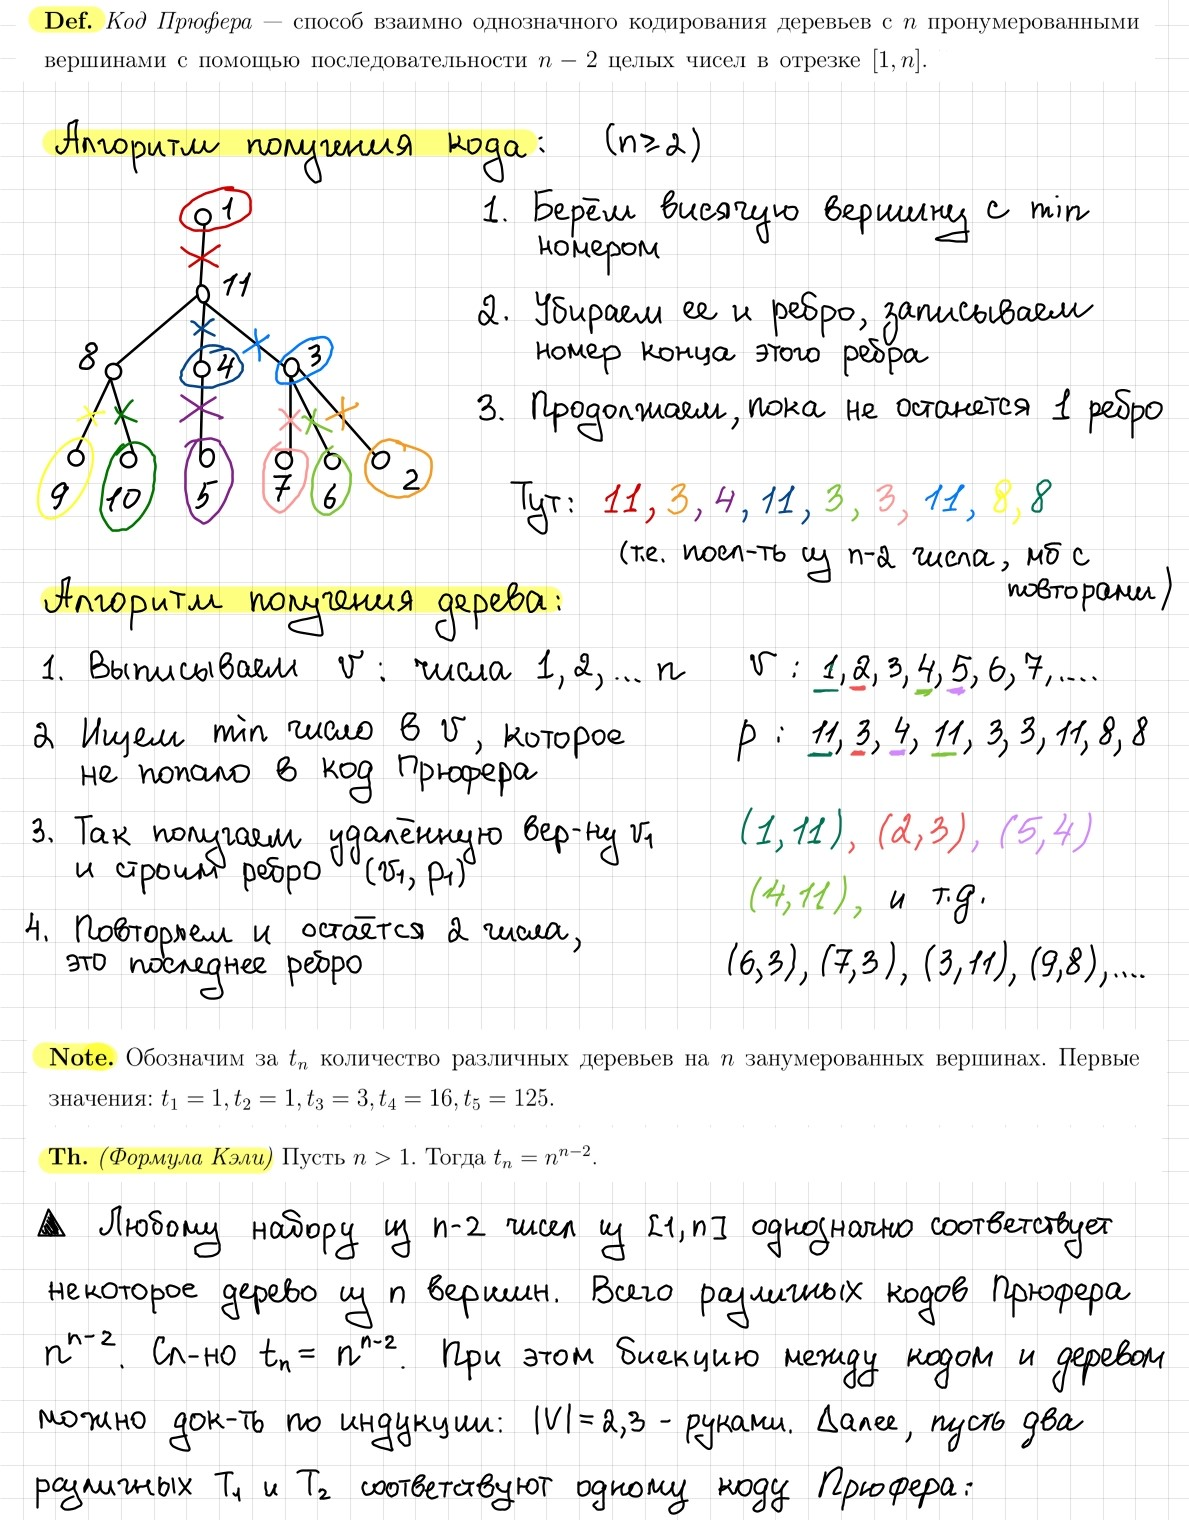
\includegraphics[width=1\linewidth]{sections/Polina/imgs/13.jpg}
\newpage 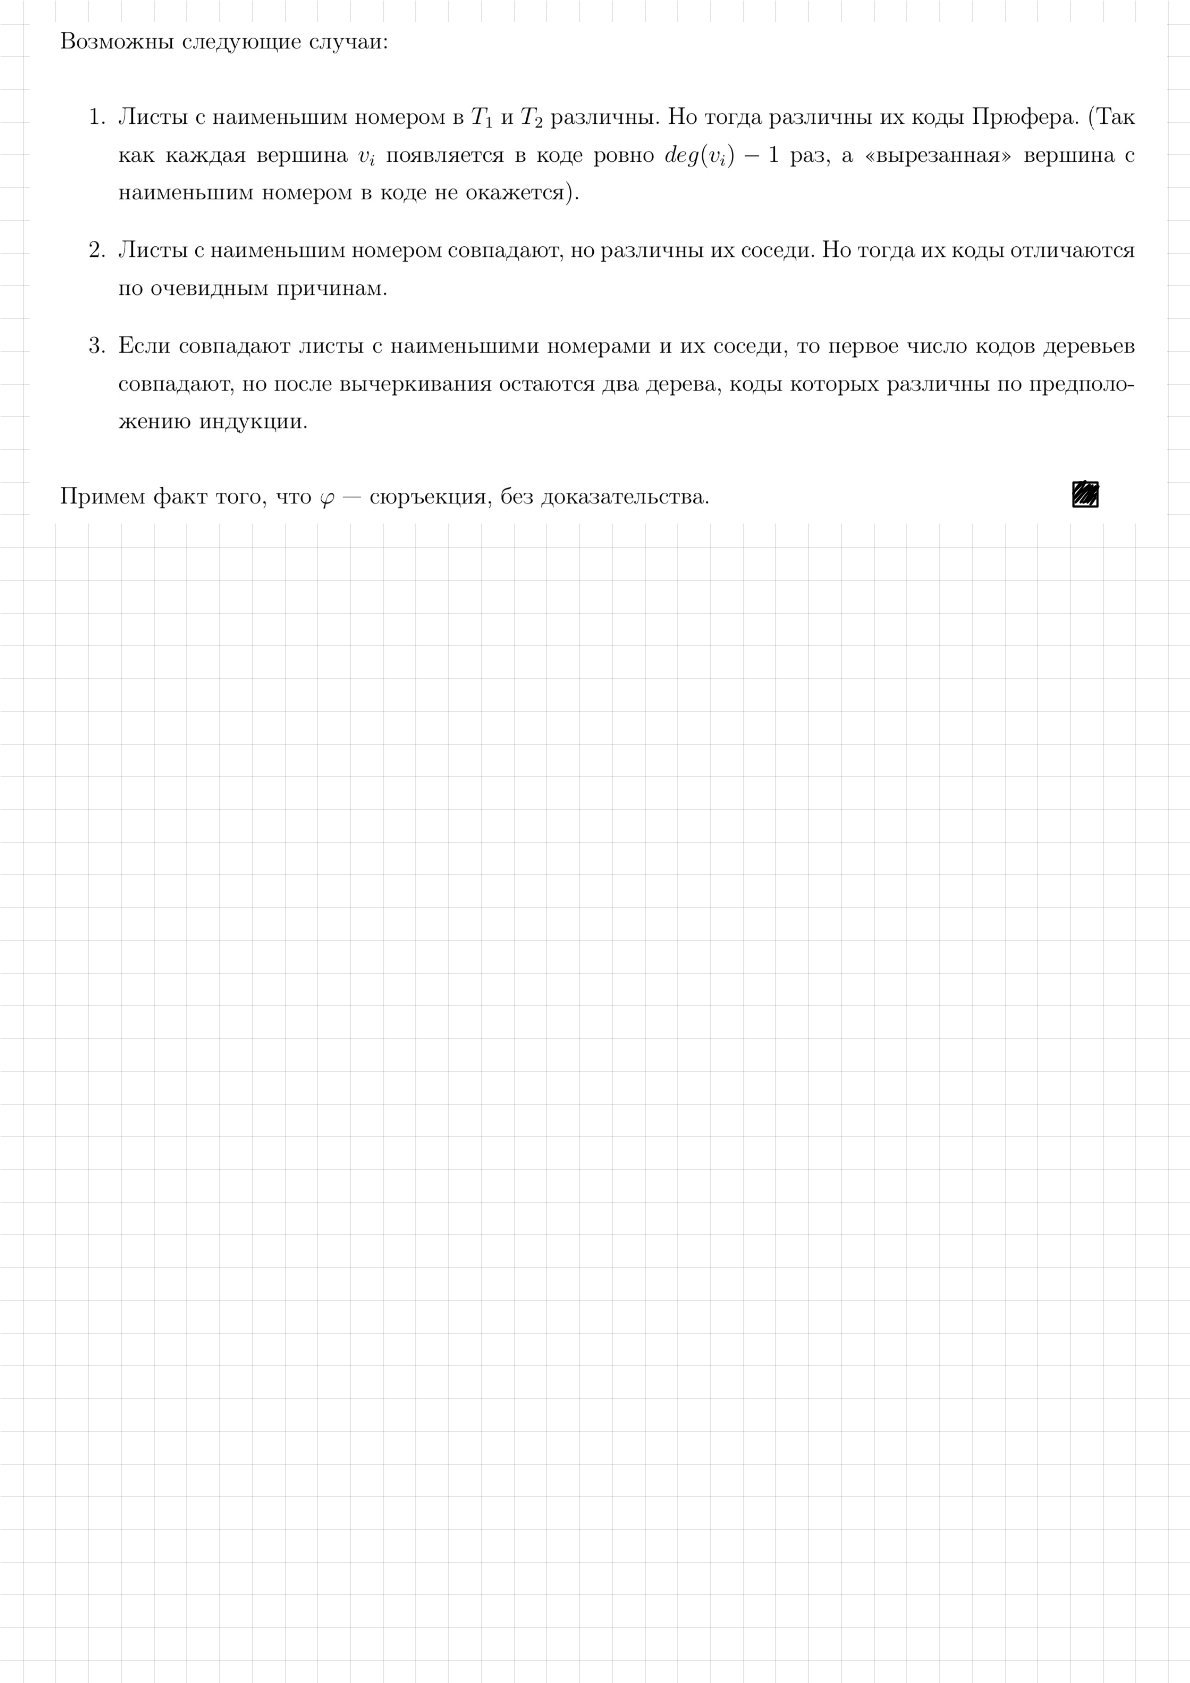
\includegraphics[width=1\linewidth]{sections/Polina/imgs/14.jpg}
\newpage{}

\subsection{3. Свойства класса автоматных языков. Замкнутость относительно булевых операций.}

\Def Полный ДКА.
Полный ДКА (ПДКА) - ДКА, для которого выполнено:
$$\forall a \in \Sigma, q \in Q \,\,\, |\Delta (q, a)| = 1$$

\Statement Для любого автоматного языка $L$ существует ПДКА $M$, такой что $L(M) = M$ (т.е. автоматы распознают одинаковое множество слов);

Метод построения ПДКА из ДКА:\\
1) строим ''стоковую'' вершину.\\
2) Добавляем из всех вершин переходы по недостающим буквам в "сток".

\begin{figure}[h]
    \hspace{-4ex} \begin{minipage}[h]{1\linewidth}
    \center{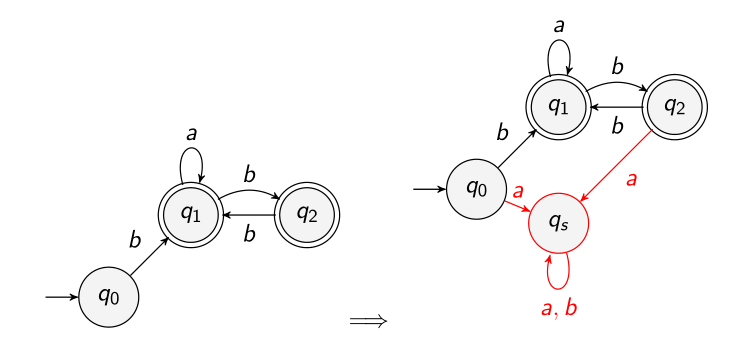
\includegraphics[width=0.6\linewidth]{1_3_1.png}}
    \end{minipage}
    \hspace{-4ex}
\end{figure}

Появятся ли новые слова? - нет, потому что, если мы попали в стоковую вершину, то не сможем ''выбраться'' из неё.

\Def Итерация Клини для языка L.
$$L^* = \cup_{k = 0}^{\infty}L^k$$

\Th Класс автоматных языков замкнут относительно\\
1. Конкатенации\\
2. Объединения\\
3. Пересечения\\
4. Итерации Клини\\
5. Дополнения

\Proof
Далее будем рассматривать только НКА с одним завершающим состоянием.
Для того чтобы после операции у итогового автомата было одно завершающее состояние, добавляем состояние и соединяем завершающие состояния с ним с помощью $\varepsilon$-переходов. (делаем новое состояние - завершающим, а старые - не завершающими)

1) Конкатенация $M_1$ и $M_2$:

Соединяем $\varepsilon$-переходами завершающее состояние $M_1$ со стартовыми состояниями $M_2$.
\begin{center}
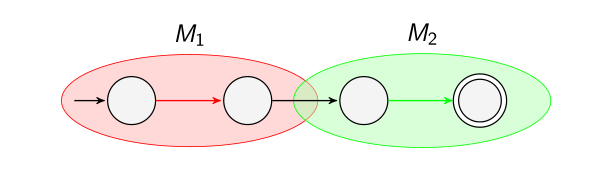
\includegraphics[width=0.45\linewidth]{1_3_2.png}
\end{center}

2) Объединение $M_1$ и $M_2$:

Добавляем стартовое состояние. Соединяем её со стартовыми состояниями $M_1$ и $M_2$ с помощью $\varepsilon$-переходов. 
\begin{center}
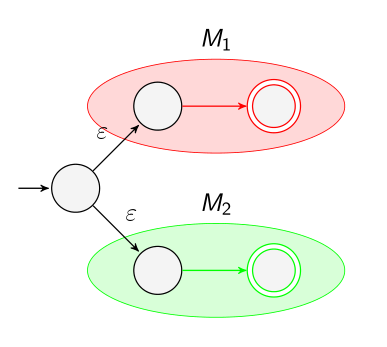
\includegraphics[width=0.25\linewidth]{1_3_3.png}
\end{center}

4) Итерации Клини над $M_1$:

Добавляем стартово-завершающее состояние. С помощью $\varepsilon$-переходов соединяем её с начальными состояниями $M_1$, а завершающее состояния $M_1$ с ней.
\begin{center}
\includegraphics[width=0.32\linewidth]{1_3_4.png}
\end{center}

3) Пересечение $M_1$, $M_2$:

Строим "декартово произведение" автоматов с одно буквенными переходами.

\begin{center}
\includegraphics[width=0.55\linewidth]{1_3_5.png}
\end{center}

То есть пересечение будет состоять из состояний, каждому из которых соответствует пара чисел $(i, j)$, это номера состояний из $M_1$ и $M_2$ соответственно, которым это состояние соответствует. И между состояниями $(i_1, j_1)$ и $(i_2, j_2)$ будет проходить ребро с символом $k$, если между $i_1$ и $i_2$ проходило ребро с символом $k$ в $M_1$ и между $j_1$ и $j_2$ проходило ребро с символом $k$ в $M_2$. $(i, j)$ - стартовое состояние, если $i$ - стартовое в $M_1$, $j$ - стартовое в $M_2$. Аналогично с завершающем состоянием. 

5) Дополнение: строим ПДКА и инвертируем терминальность всех состояний.

\newpage{}

\subsection{4. Регулярные выражения. Теорема Клини о совпадении классов регулярных и автоматных языков. Регулярный автомат, алгоритм построения.}

\Vars \\
Regex (регулярное выражение) обозначим за $R$, \newline Language (язык) -- за $L$, \newline $L(R_i)$ (язык, который задается регулярным выражением $R$) -- $L_i$.

\Def Рекурсивное определение регулярного выражения.

% \begin{minipage}[r]{0.1\linewidth} 
% %\begin{flushright}
%     \includegraphics[width=5\linewidth]{images/1_4_1.png}
% %\end{flushright} 
% \end{minipage} 
\begin{center}
    \begin{tabular}{|c|c|}
        \hline
        $Regex (R)$ & $Language (L_i = L(R_i))$ \\
        \hline
        $0$ & $\varnothing$ \\
        $1$ & $\{ \varepsilon \}$ \\
        $a$, $a \in \Sigma$ & $\{ a \}$ \\
        $R_1 + R_2$ & $L_1 \cup L_2$ \\
        $R_1 \cdot R_2$ & $L_1 \cdot L_2$ \\
        $R^*$ & $L^*$ \\
        \hline
    \end{tabular}
\end{center}

Здесь $\varepsilon$ -- пустое слово, <<$\cdot$>> -- операция конкатенации языков (в полученном языке $L_1 \cdot L_2$ лежат слова вида $a_1a_2$, где слово $a_1$ лежит в языке $L_1$, а слово $a_2$ лежит в языке $L_2$), <<$*$>> -- звезда Клини.

Напомним определение звезды Клини: $V^* = \bigcup_{i=0}^{\infty} V^i$ 

\textbf{Приоритет операций} в регулярных выражениях (левее — приоритетнее): $* \rightarrow \cdot \rightarrow +$

\Def Язык $L$ -- регулярный, если он задается регулярным выражением.

\hspace{4ex}

\textbf{Теорема Клини:} Классы регулярных и автоматных языков совпадают.

\Proof Докажем два вложения:

\textbf{1. Регулярные $\subseteq$ Автоматные}

% \begin{figure}[h]
%     \begin{minipage}[h]{0.6\linewidth}
%     Индукция по построению выражения. 
    
%     Немного изменим утверждение -- докажем, что по регулярному выражению можно построить НКА с $1$ завершающим состоянием, который задает тот же язык.\\
    
%     \textit{База}: Построим автоматы для регулярных выражений: 0, 1, a.
%     \end{minipage}
%     \hspace{-4ex} \begin{minipage}[h]{0.5\linewidth}
%     \center{\includegraphics[width=0.6\linewidth]{images/4_base.jpg}}
%     \end{minipage}
% \end{figure}
% Регулярное выражение <<$0$>> -- автомат без завершающих состояний.

% Регулярное выражение <<$1$>> -- в автомате, состоящем из одной вершины, стартовая вершина помечается завершающим состоянием.

% Регулярное выражение <<$a$>> -- в автомате две вершины. Вершина номер $0$ стартовая, вершину номер $1$ помечаем как терминальную. Проводим ребро из $0$ в $1$, на котором пишем букву a.

Индукция по построению выражения. Немного изменим утверждение -- докажем, что по регулярному выражению можно построить НКА с $1$ завершающим состоянием, который задает тот же язык.

\textit{База}: Построим автоматы для регулярных выражений: $0, 1, a \in \Sigma$.
% %картинка%
\begin{figure}[h!]
    \centering
    \includegraphics[scale=0.27]{4_base.jpg}
\end{figure}
% \newline \center{\includegraphics[width=0.29\linewidth]{4_base.jpg}}
% \begin{minipage}[r]{1\linewidth} 
% %\begin{flushright}
%     % \includegraphics[width=2\linewidth]{images/1_4_2.png}
%     \center{\includegraphics[width=1\linewidth]{images/4_base.jpg}}
% %\end{flushright} 
% \end{minipage} 

\textit{Переход:}

1) $R = R_1 + R_2$. Построим автомат $A_1$ для $R_1$, для которого вершина $S_1$ -- стартовая, а вершина $F_1$ -- единственная терминальная. Для $R_2$ это будут автомат $A_2$ со стартовой вершиной $S_2$ и терминальной $F_2$.
Создадим новую вершину $S$, которая и будет стартовой в новом автомате. Из нее проведем два ребра с $\varepsilon$-переходами в $S_1$ и в $S_2$. Аналогично соединим завершающие в автоматах с новой завершающей вершиной $F$. Нетрудно доказать, что такой автомат задаст тот же язык, что и наше регулярное выражение.

2) $R = R_1 \cdot R_2$. Аналогично прошлому пункту получим автоматы для $R_1$ и $R_2$ с теми же обозначениями. Вершина $S_1$ будет стартовой в нашем новом автомате. Добавим также $\varepsilon$-переход из $F_1$ в $S_2$, уберем терминальность $F_1$.

3) $R = R_1^*$. Построим автомат $A_1$ для $R_1$ со стартовой вершиной $S_1$ и терминальной вершиной $F_1$. Создадим вершину $S$ -- новую стартовую вершину, пометим ее терминальной. Добавим из нее и из $F_1$ $\varepsilon$-переход в $S_1$.

\textbf{2. Автоматные $\subseteq$ Регулярные}

\Note{Регулярный автомат -- НКА, в котором на ребрах записаны регулярные выражения. Докажем утверждение для регулярных автоматов.}

\Note{Всякий НКА задается регулярным автоматом с 1 завершающим состоянием.}

Индукция по $|Q|$ (количеству состояний -- вершин) в регулярном автомате.

\textit{База:}

1) $|Q| = 1$. Тогда в регулярном автомате стартовое состояние является завершающим, и можно однозначно построить регулярное выражение. Такому автомату соответсвует регулярное выражение $a^*$
\newline
\begin{minipage}[r]{0.1\linewidth} 
%\begin{flushright}
    \includegraphics[width=4\linewidth]{images/1_4_3.png}
%\end{flushright} 
\end{minipage} 

2) $|Q| = 2$. Cтартовое состояние и завершающее состояние различны, и можно тоже однозначно построить регулярное выражение. Такому автомату соответсвует регулярное выражение $\alpha^*\beta(\gamma + \delta \alpha^* \beta)^*$
\newline
\begin{minipage}[r]{0.1\linewidth} 
%\begin{flushright}
    \includegraphics[width=4\linewidth]{images/1_4_4.png}
%\end{flushright} 
\end{minipage} 

Для случая, когда завершающее состояние -- это начальная вершина, регулярное выражение будет $(\gamma + \delta \alpha^* \beta)^*$.

\textit{Переход:}
\Note{Есть нестартовая и незавершающая вершина!}

1) Удаляем кратные ребра:
\begin{minipage}[r]{0.2\linewidth} 
%\begin{flushright}
    \includegraphics[width=2.5\linewidth]{images/1_4_5.png}
%\end{flushright} 
\end{minipage} 

Кратные ребра означают, что мы можем выбрать, какой символ будем использовать. Именно этот смысл и несет в себе операция <<$+$>>.

2) Добавляем циклы на себя:
\begin{minipage}[r]{0.1\linewidth} 
%\begin{flushright}
    \includegraphics[width=3.5\linewidth]{images/1_4_6.png}
%\end{flushright} 
\end{minipage} 

3) Удаляем нестартовое и незавершающее состояние:

\begin{minipage}[r]{0.1\linewidth} 
%\begin{flushright}
    \includegraphics[width=5.5\linewidth]{images/1_4_7.png}
%\end{flushright} 
\end{minipage} 
\newline Теперь у нас на одно сотояние стало меньше, т.е. мы можем воспользоваться утверждением индукции.
\EndProof
\newpage{}

\subsection{5. Минимальный ДКА, его существование.}

\textbf{Мотивировка:} может быть много состояний. А еще не очень понятно, как сравнивать два автомата на эквивалентность. Вернее, если проверять <<в лоб>>, будет долго. Один из способов решить эти проблемы -- минимизация автомата.\\

Пусть $L \subset \Sigma^*$ -- автоматный язык, $M$ -- ПДКА для $L$.

\Def Минимальный ПДКА $M$, распознающий язык $L$, если $M$ -- минимальный по количеству состояний.

\hspace{4ex}

\Def Определим отношение эквивалентности $\sim_L$ на $\Sigma^*:$
$$u \sim_L v \Longleftrightarrow \forall w \in \Sigma^* \,\,(uw \in L \Longleftrightarrow vw \in L)$$

Определение корректно (рефлексивность, симметричность и транзитивность очевидны).

\textit{Множество классов эквивалентности в этом случае:} 
$\Sigma^* /_{\sim_L}:= \{\{u \arrowvert u \sim_L v\} \,\,\arrowvert\,\, v \in \Sigma^*\}$

\Def Определим отношение эквивалентности $\sim_M$ на $Q:$
$$q_1 \sim_M q_2 \Longleftrightarrow \forall w \in \Sigma^*\,\,(\Delta(q_1, w) \in F \Longleftrightarrow \Delta(q_2, w) \in F)$$

Если $q_1 \sim_M q_2$, то состояния можно объединить.

\textit{Напоминание:} Множество вершин, достижимых из $q$ по $w$ -- $\Delta (q, w) = \{ q' | \langle q, w \rangle \vdash \langle q', \varepsilon \rangle \}$..\\

% \hspace{4ex} 
\textbf{Лемма}
Пусть $L_q := \{w \,\arrowvert\, \Delta(q_0, w) = q\}$. Тогда каждый класс эквивалентности в нашем фактор-множестве являетеся объединением классов в $L_q$.

\Proof
Возьмем слово $u \in [u] \in \Sigma^*/_{\sim_L}$, где $[u]$ -- это класс эквивалентности для $u$. Рассмотрим путь по $u$ из $q_0$, а именно,  $q_u = \Delta(q_0, u)$. Для любого слова $w \in [u]$, $q_w = \Delta \brackets{q_0, w}$. Тогда $[u] = \bigcup \limits_{q_w, w \in [u]} L_{q_w}$. Далее докажем, почему это так.
% Из последнего очевидно, что $u \in L_{q_u}$. 

Пусть $v \in [u] \,\Longrightarrow\, v \sim_L u \,\Longrightarrow\, q_v = \Delta \brackets{q_0, v} \,\Longrightarrow\, v \in L_{q_v}$. Тогда $v \in \bigcup \limits_{q_w, w \in [u]} L_{q_w}$.

Пусть $v \in \bigcup \limits_{q_w, w \in [u]} L_{q_w}$. Тогда существует состояние $q_z$, $z \in [u]$, что $v \in L_{q_z} = \{ w | \Delta \brackets{q_0, w} = q_z \}$.
\begin{center}
    $z \in [u] \Longrightarrow z \sim_L u \stackrel{def}{\Longrightarrow} \; \forall w \in \Sigma^* \; \brackets{zw \in L \Longleftrightarrow uw \in L}$
    \begin{equation*}
        \left.
          \begin{array}{ccc}
            v \in L_{q_z} \Longrightarrow & \Delta \brackets{q_0, v} & = q_z \\
            & \Delta \brackets{q_0, z} & = q_z \\
          \end{array}
        \right\} \quad
    \Longrightarrow \quad v \sim_L z \text{ так как $\forall w \in \Sigma^*$ $\Delta \brackets{q_0, vw} \stackrel{(*)}{=} \Delta \brackets{q_0, zw}$}
    \end{equation*}
\end{center}

$\brackets{*}$: $\Delta \brackets{q_0, vw} = \Delta \brackets{\Delta(q_0, v), w} = \Delta \brackets{q_z, w} = \Delta \brackets{\Delta(q_0, z), w} = \Delta \brackets{q_0, zw}$

Так как $v \sim_L z$, $z \in [u]$, то $v \in [u]$. Значит, $[u] = \bigcup \limits_{q_w, w \in [u]} L_{q_w}$, и каждый класс эквивалентности из $\Sigma^* /_{\sim_L}$ — объединение классов в $L_q$. \quad \EndProof

% И так для любого элемента $w \in [u] \hookrightarrow w \in L_{q_w}$. Поэтому \[ [u] \subset \bigcup_{q_w, w \in [u]} L_{q_w}.\]

% Докажем теперь обратное включение. Возьмем $v \in L_{q_w}$. Для него верно $q_v = \Delta(q_0, v) = q_w$. Докажем, что тогда $v \in [w]$ ($[u] = [w]$).

% Возьмем произвольное $m \in \Sigma^*$. Заметим, что тогда верно $vm \in L \Longleftrightarrow wm \in L$, ведь слово $w$ читается из состояния $q_v$ и приводит в завершающее тогда и только тогда, когда то же самое верно и для $q_w$ (просто в силу того, что $q_v = q_w$).


\textbf{Следствие}
$\arrowvert \Sigma^*/_{\sim_L} \arrowvert \leq \arrowvert Q \arrowvert$\\

\textit{Теперь перейдем к минимальному ПДКА, а именно докажем его существование (тут) и единственность с точностью до изоморфизма (билет 6).}\\

\textbf{Лемма} Для любого автоматного языка $L$ существует ПДКА $M'$ такой, что все состояния в $M'$ попарно неэквивалентны.

Что необходимо доказать?\\
1) Переходы и завершающие состояния согласованы\\
2) Распознаваемые языки совпадают\\
3) Состояния попарно неэквивалентны

\Proof Рассмотрим автомат над классами эквивалентности $\sim_M$. Класс эквивалентности $q$ обозначим за $[q]$. $M' = \langle Q /_{\sim_M}, \Sigma, \Delta', [q_0], F' \rangle$, где:

\begin{center}
    $\Delta' = \{ \langle [q_1], a \rangle \rightarrow [q_2] \;|\; \exists \langle q_1, a \rangle \rightarrow q_2 \in \Delta \}$
    
    $F' = \{ [q_f] \;|\; q_f \in F \}$
\end{center}

1) Проверим, что множества $\Delta'$, $F'$ заданы корректно.

Для $\Delta'$: Пусть $q_1 \sim_m q_1'$, и существует $a$ такое, что $\Delta \brackets{q_1, a} \nsim_m \Delta \brackets{q_1', a}$.
\begin{center}
    $q_1 \sim_M q_1' \stackrel{def}{\Longrightarrow} (\forall w \in \Sigma^* \;\;\Delta \brackets{q, w} \in F \Longleftrightarrow \Delta \brackets{q_1', w} \in F)$
    
    $w = au \Longrightarrow (\forall u \in \Sigma^* \;\; \Delta \brackets{q_1, au} \in F \Longleftrightarrow \Delta \brackets{q_1', au} \in F)$
\end{center}

Далее обозначим $\Delta \brackets{q_1, a} = q_2$, a $\Delta \brackets{q_1', a} = q_2'$.
\begin{center}
    $\Delta \brackets{q_1, au} = \Delta \brackets{\Delta(q_1, a), u} = \Delta \brackets{q_2, u}$
    
    $\Delta \brackets{q_1', au} = \Delta \brackets{q_2', u}$
    
    $(\Delta \brackets{q_2, u} \in F \Longleftrightarrow \Delta \brackets{q_2', u} \in F)\; \Longrightarrow q_2 \sim_m q_2'$.
\end{center}

Приходим к противоречию.

Для $F'$:
\begin{center}
    $q_1 \in F$, $q_2 \sim_M q_1 \overset{w = \varepsilon}{\Longrightarrow} (\Delta \brackets{q_1, \varepsilon} \in F \Longleftrightarrow \Delta \brackets{q_2, \varepsilon} \in F)$
    
    Значит, $q_1 \in F \Longleftrightarrow q_2 \in F$
\end{center}

2) Теперь покажем, что $L \brackets{M} = L \brackets{M'}$. 

Для этого нужно показать, что $w \in L \brackets{M} \Longleftrightarrow \Delta \brackets{q_0, w} \in F \stackrel{?}{\Longleftrightarrow} \Delta \brackets{[q_0], w} \in F'$.

Докажем утверждение: $\forall u: \Delta \brackets{q_0, u} = q_1 \Longleftrightarrow \Delta \brackets{[q_0], u} = [q_1]$.

Индукция по длине слова $u$.

\textbf{База.} $|u| = 0 \Longrightarrow u = \varepsilon$. Тогда $\Delta \brackets{q_0, \varepsilon} = q_0$, $\Delta \brackets{[q_0], \varepsilon} = [q_0]$.

\textbf{Переход.} Пусть $u = va$, $v \in \Sigma^*$, $a \in \Sigma$.

\begin{center}
    $\Delta \brackets{q_0, va} = q_1 \Longrightarrow \exists q_2\; \Delta \brackets{q_0, v} = q_2, \;\Delta \brackets{q_2, a} = q_1$
\end{center}

По предположению индукции, $\Delta \brackets{[q_0], u} = [q_2]$, $\Delta \brackets{[q_2], a} = [q_1]$, так как переход $\langle q_2, a \rangle \rightarrow q_1 \in \Delta$ тогда и только тогда, когда $\langle [q_2], a \rangle \rightarrow [q_1] \in \Delta'$. По транзитивности, $\Delta \brackets{[q_0], ua} = [q_1]$.

3) Теперь покажем, что состояния попарно неэквивалентны. В автомате, построенном на классах эквивалентности состояний никакие два состояния не эквивалентны, потому что тогда бы они лежали в одном классе, т.е. были бы одним состоянием.

Пусть $[q_1] \sim_{M'} [q_2]$. Тогда $\forall w : \Delta_{M'} \brackets{[q_1], w} \in F' \Longleftrightarrow \Delta_{M'} \brackets{[q_2], w} \in F'$ по определению. 

\begin{center}
    $[q_{1f}] = \Delta_{M'} \brackets{[q_1], w} \in F'$
    
    $[q_{2f}] = \Delta_{M'} \brackets{[q_2], w} \in F'$
    
    $\exists q_{1f} \in F : \Delta_M \brackets{q_1, w} = q_{1f} \in F \Longleftrightarrow \exists q_{2f} \in F : \Delta_M \brackets{q_2, w} = q_{2f} \in F$
    
    $q_1 \sim_{M} q_2 \Longrightarrow [q_1] = [q_2]$
\end{center}
\begin{flushright}
  \EndProof
\end{flushright} 


\Th $M$ — минимальный ПДКА, распознающий язык $L$, тогда и только тогда, когда любые два состояния попарно неэквивалентны и все состояния достижимы из стартового.

\textit{Теперь запишем более формально:}

\begin{center}
    $M$ — минимальный ПДКА $\Longleftrightarrow \begin{cases} \forall q_1, q_2 \in Q \ q_1 \nsim q_2 \\ \forall q \in Q \ \exists w \in \Sigma^* : \ \langle q_0, w \rangle \vdash \langle q, \varepsilon \rangle \end{cases}$
\end{center}

\Proof

$\Longrightarrow$ Если $q_1 \sim_M q_2$, то $[q_1] = [q_2]$, и их можно объединить в одно состояние, значит, $M$ не был бы минимальным, и тогда из минимальности следует, что $q_1 \nsim_M q_2$. Если среди состояний есть недостижимые, то если их удалить, то множество принимаемых слов не изменится.

$\Longleftarrow$ По следствию из леммы о $L_q$: $|\Sigma^* /_{\sim_L}| \leqslant |Q|$. Рассмотрим $w_1$, $w_2$ такие, что $\Delta \brackets{q_0, w_1} \neq \Delta \brackets{q_0, w_2}$. Введём обозначения:

\begin{center}
    $\Delta \brackets{q_0, w_1} = q_1$
    
    $\Delta \brackets{q_0, w_2} = q_2$
\end{center}

Неэквивалентность состояний $q_1$, $q_2$ означает, что существует слово $w$, что б.о.о:

\begin{center}
    $\Delta \brackets{q_1, w} = \Delta \brackets{q_0, w_1 w} \in F \Longleftrightarrow w_1 w \in L$
    
    $\Delta \brackets{q_2, w} = \Delta \brackets{q_0, w_2 w} \notin F \Longleftrightarrow w_2 w \notin L$
    
    Следовательно, получили что $w_1 \nsim_L w_2$
\end{center}

Тогда для автомата $M$ со множеством состояний $Q'$ выполняется, что $|\Sigma^* /_{\sim_L}| \geqslant |Q'|$, но тогда $|Q| \geqslant |\Sigma^* /_{\sim_L}| \geqslant |Q'|$, и $M$ — минимальный. \quad \EndProof
\newpage{}

\includegraphics[width=1\linewidth]{sections/Polina/imgs/25.jpg}
\newpage{}

\setcounter{section}{6}

\section{Понятия образа и прообраза множества при соответствии. Критерий равенства образа пересечения и пересечения образов. Аналогичные критерии с объединением и разностью.} 
\textbf{Соответствие} между множествами A и B - произвольное подмножество декартова произведения $F \subset A \times B$. Обозначение: $F: A \to B$; иногда, чтобы подчеркнуть, что одному элементу из A может соответствовать несколько элементов из B, пишут: $F:A\rightrightarrows B$. 
\\
\par
Пусть $F: A \to B$ - соответствие, $S \subset A$, $T \subset B$. Тогда \textbf{образ} множества S - множество всех элементов B, соответствующих какому-то элементу S. Формально: $F(S) = \bigcup_{s \in S} F(s) \subset B $. \textbf{Прообраз} множества Т - множество элементов А, которым соответсвует хотя бы один элемент Т. Формально: $F^{-1}(T) = \left\{ a: F(a) \cap T \neq \varnothing \right\}$ 
\\
\par
\emph{ Образ пересечения любых двух множеств равняется пересечению образов тех же множеств $\iff$ соответствие инъективно. } 
\\
$\blacktriangle$
Пусть соответствие не инъективно. Тогда найдутся такие $a_1$ и $a_2$, что $F(a_1)$ и $F(a_2)$ пересекаются. Тогда $F(\left\{a_1\right\} \cap \left\{a_1\right\}) = F(\varnothing) = \varnothing$, но $F(\left\{a_1\right\}) \cap F(\left\{a_2\right\}) = F(a_1) \cap F(a_2)$ не пуст по предположению. Значит, образ пересечения множеств $\left\{ a_1\right\}$ и $\left\{ a_2\right\}$ не равен пересечению образов. \par
Теперь пусть соответствие инъективно. Рассмотрим произвольные подмножества S и Q множества А. Докажем, что $F(S \cap Q) = F(S) \cap F(Q)$. Для этого докажем включение в обе стороны. Вначале пусть $y \in F(S \cap Q)$. Это значит, что $y \in F(x)$ для некоторого $x \in S \cap Q$. Тогда $x \in S$ и $x \in Q$. А раз $y \in F(x)$, то $y \in F(S)$ и $y \in F(Q)$. Значит, $y \in F(S) \cap F(Q)$. (Это включение верно для всех соответствий). \par
Теперь пусть $y \in F(S) \cap F(Q)$. Значит, $y \in F(x_1)$ для некоторого $x_1 \in S$ и $y \in F(x_2)$ для некоторого $x_2 \in Q$. Но при $x_1 \neq x_2$ в силу инъективности множества $F(x_1)$ и $F(x_2)$ не пересекаются. А их пересечение содержит хотя бы y. Значит, $x_1 = x_2 = x$, и $x \in S \cap Q$. А так как $y \in F(x)$, то получаем $y \in F(S \cap Q)$.
$\blacksquare$ \\
\par
\emph{ Образ объединения любых двух множеств равняется объединению образов тех же множеств - выполняется для любых соответствий. } \\
$\blacktriangle$
1) $\left.
  \begin{array}{ccc}
    A \subseteq A \cup B \Rightarrow F(A) \subseteq F(A \cup B) \\
    B \subseteq A \cup B \Rightarrow F(B) \subseteq F(A \cup B) \\
  \end{array}
\right\} \Rightarrow F(A) \cup F(B) \subseteq F(A \cup B) $ \\
2) $y \in F(A \cup B) \Rightarrow \exists x \in A \cup B: y = F(x) \Rightarrow \exists x \in A \cup x \in B: y = F(x) \Rightarrow$ \\
$\Rightarrow y \in F(A) \cup y \in F(B) \Rightarrow y \in F(A) \cup F(B) \Rightarrow  F(A \cup B) \subseteq F(A) \cup F(B) $; \\
Из пунктов 1 и 2 следует, что $F(A \cup B) = F(A) \cup F(B) $
$\blacksquare$ \\
\par
\emph{ Образ разности любых двух множеств равняется разности образов тех же множеств $\iff$ соответствие инъективно. } \\
Доказательство аналогично доказательству для пересечения.
\newpage{}

\includegraphics[width=1\linewidth]{sections/Polina/imgs/5.jpg}
\newpage{}

\setcounter{section}{8}
\section{Проверка правильности скобочной последовательности с несколькими типами скобок.}
\par \textbf{Определение}: \textit{Правильные скобочные последовательности с несколькими типами скобок} (рассмотрим с двумя)
\begin{enumerate}
    \item $\varepsilon$ (пустое слово) - ПСП
    \item $S$ - ПСП $\Rightarrow (S), [S]$ - ПСП
    \item $S_1, S_2$ - ПСП $\Rightarrow S_1 S_2$ - ПСП 
\end{enumerate}
\par \textbf{Задача:} Проверить, является ли последовательность из нескольких типов скобок правильной скобочной последовательностью
\par \textbf{Решение:} Храним стек незакрытых открывающих скобок
\lstinputlisting[language=C++,
emph={int,char,double,float,unsigned},
emphstyle={\color{blue}}
]{code/9_psp.cpp}
\par \textbf{Утверждение:} Данный алгоритм корректен, то есть ПСП $\Leftrightarrow$ алгоритм вывел true
\begin{itemize}
    \item[$\blacktriangle \Rightarrow$] Индукция по построению \begin{enumerate}
    \item База: $\varepsilon$ - обработается корректно
    \item $T=(u)$, $u$ - ПСП. По предположению индукции, всё $u$ удалится из стека к моменту прихода закрывающей скобки (можно считать, что стек начинается после первой скобки, она никак не влияет на применение алгоритма к $u$), а внешние скобки обработаются корректно (аналогично для других типов скобок)
    \item $T=T_1 T_2; T_1, T_2$ - ПСП. По предположению индукции, после того как считается $T_1$ стек опустошится $\Rightarrow$ после $T_2$ - тоже $\Rightarrow$ алгоритм сработает корректно $\blacksquare$
    \end{enumerate}
    \item[$\Leftarrow$] Доказываем индукцией по количеству действий, "обращая" предыдущий пункт.
    \par Рассмотрим скобочную последовательность, на которую алгоритм выдаёт true. Алгоритм сопоставил каждой открывающейся скобке одного типа закрывающуюся скобку того же типа. Причём они обязательно идут в правильном порядке. 
\parДля доказательства факта используем индукцию.
Рассмотрим пары соответсвующих скобок в порядке закрытия пары:
\begin{enumerate}
    \item База: Если между парой скобок нет других скобок, то последовательность от одной скобки до другой - правильная.
    \item Шаг: Если между парой скобок (назовём их $a$ и $b$ соответственно) есть непустая подстрока, то все скобки из подстроки уже были рассмотрены индукцией, так как открывающиеся скобки в подстроке были позже, чем $a$ добавлены в стек и по правилу стека должны были раньше из него выйти, а значит они уже были рассмотрены индукцией. Аналогично с закрывающимеся скобками из подстроки - они идут раньше, чем $b$, следовательно, по правилу стека им ставили в соответствие открывающиеся скобки, которые были добавленны позже $a$. (окрывающаяся скобка не могла быть добавленны раньше $a$, потому что $a$ перегородила бы ей выход.) По предположению индукции получаем, что подстрока состоит из одной или нескольких ПСП $\Rightarrow$ сама подстрока ПСП. $\Rightarrow$ Подпоследовательность от $a$ до $b$ - правильная. $\blacksquare$
\end{enumerate}
\end{itemize} 
\newpage{} 
    
\mysection{4}{4. Конечные преобразователи}
    \section{Асимптотические обозначения: $O, \Omega, \Theta$. Независимость от стартового индекса. Мастер-теорема (б/д).}
\par \textbf{Определение:} Пусть $f,g: \; \mathbb{N} \rightarrow \mathbb{N}$. Тогда $f=O(g)$, если существует $c, N$, такие что $\forall n \in N \; \hookrightarrow n \geqslant N \Rightarrow f(n) \leqslant c \cdot g(n)$.
\par \textbf{Определение:} Пусть $f,g: \; \mathbb{N} \rightarrow \mathbb{N}$. Тогда $f=\Omega(g)$, если существует $c, N$, такие что $\forall n \in N \; \hookrightarrow n \geqslant N \Rightarrow f(n) \geqslant c \cdot g(n)$.
\par \textbf{Замечание:} $f = \Omega(g) \Leftrightarrow g = O(f)$
\par \textbf{Определение:} Пусть $f,g: \; \mathbb{N} \rightarrow \mathbb{N}$. Тогда $f=\Theta(g)$, если существует $c_1,c_2, N$, такие что $\forall n \in N \; \hookrightarrow \\ n \geqslant N \Rightarrow c_1 \cdot g(n) \leqslant f(n) \leqslant c_2 \cdot g(n)$.
\par \textbf{Замечание:} $f = \Theta(g) \Leftrightarrow f = O(g)$ и $f = \Omega(g)$
\par \textbf{Утверждение:} $f = O(g) \Leftrightarrow \exists c: \forall n \in \mathbb{N} \hookrightarrow f(n) \leqslant c \cdot g(n)$ 
\par \begin{itemize}
    \item[$\blacktriangle \Leftarrow$] Очевидно, достаточно положить $N=1$
    \item[$\Rightarrow$] Пусть $\forall n \geqslant N \hookrightarrow f(n) \leqslant c \cdot g(n)$. Определим $c'=\max \{c, \frac{f(1)}{g(1)}, \ldots, \frac{f(N)}{g(N)}\}$ ($g$ не обращается в 0 так как результат натуральный). Тогда \begin{enumerate}
        \item $n \geqslant N \Rightarrow f(n) \leqslant c \cdot g(n) \leqslant c' \cdot g(n)$
        \item $n < N \Rightarrow c' \geqslant \frac{f(n)}{g(n)} \Rightarrow f(n) \leqslant c' \cdot g(n) \; \blacksquare$
    \end{enumerate}
\end{itemize}
\par Для $\Omega$ и $\Theta$ справедливы аналогичные утверждения.
\par \textbf{Мастер-теорема (с лекции):} Пусть $T: \mathbb{N} \rightarrow \mathbb{N}$ с условием $T(n)=a \cdot T(\frac{n}{b})+f(n)$, $a=const, a \geqslant 1; \\ b=const, b \geqslant 1, f: \mathbb{N} \rightarrow \mathbb{N}$. Тогда \begin{enumerate}
    \item Если $\exists \varepsilon > 0$, такое что $f(n)=O(n^{\log_b a - \varepsilon})$, то $T(n)=\Theta(n^{\log_b a})$
    \item Если $f(n)=\Theta(n^{\log_b a})$, то $T(n)=\Theta(n^{\log_b a} \log n)$
    \item Если $\exists \varepsilon > 0$, такое что $f(n)=\Omega(n^{\log_b a + \varepsilon})$, причем $\exists c < 1$, такое что $a \cdot f(\frac{n}{b}) \leqslant c \cdot f(n)$ для всех $n$, начиная с некоторого номера, то $T(n)=\Theta(f(n))$
\end{enumerate}
\par \textbf{Мастер-теорема (из интернета):} Пусть имеется рекуррентное соотношение:
$$T(n)=\left\{
\begin{array}{ccc}
a \cdot T(\frac{n}{b})+O(n^c), n>1\\
O(1),n=1\\
\end{array}
\right., \text{ где } a \in \mathbb{N}, b \in \mathbb{R}, b>1, c \in R^+.$$

Тогда асимптотическое решение имеет вид: \begin{enumerate}
    \item Если $c>\log_b a$, то $T(n)=O(n^c)$
    \item Если $c=\log_b a$, то $T(n)=O(n^c \log n)$
    \item Если $c<\log_b a$, то $T(n)=O(n^{\log_b a})$
\end{enumerate}
\newpage{}

\includegraphics[width=1\linewidth]{sections/Polina/imgs/13.jpg}
\newpage \includegraphics[width=1\linewidth]{sections/Polina/imgs/14.jpg}
\newpage{}

\subsection{3. Свойства класса автоматных языков. Замкнутость относительно булевых операций.}

\Def Полный ДКА.
Полный ДКА (ПДКА) - ДКА, для которого выполнено:
$$\forall a \in \Sigma, q \in Q \,\,\, |\Delta (q, a)| = 1$$

\Statement Для любого автоматного языка $L$ существует ПДКА $M$, такой что $L(M) = M$ (т.е. автоматы распознают одинаковое множество слов);

Метод построения ПДКА из ДКА:\\
1) строим ''стоковую'' вершину.\\
2) Добавляем из всех вершин переходы по недостающим буквам в "сток".

\begin{figure}[h]
    \hspace{-4ex} \begin{minipage}[h]{1\linewidth}
    \center{\includegraphics[width=0.6\linewidth]{1_3_1.png}}
    \end{minipage}
    \hspace{-4ex}
\end{figure}

Появятся ли новые слова? - нет, потому что, если мы попали в стоковую вершину, то не сможем ''выбраться'' из неё.

\Def Итерация Клини для языка L.
$$L^* = \cup_{k = 0}^{\infty}L^k$$

\Th Класс автоматных языков замкнут относительно\\
1. Конкатенации\\
2. Объединения\\
3. Пересечения\\
4. Итерации Клини\\
5. Дополнения

\Proof
Далее будем рассматривать только НКА с одним завершающим состоянием.
Для того чтобы после операции у итогового автомата было одно завершающее состояние, добавляем состояние и соединяем завершающие состояния с ним с помощью $\varepsilon$-переходов. (делаем новое состояние - завершающим, а старые - не завершающими)

1) Конкатенация $M_1$ и $M_2$:

Соединяем $\varepsilon$-переходами завершающее состояние $M_1$ со стартовыми состояниями $M_2$.
\begin{center}
\includegraphics[width=0.45\linewidth]{1_3_2.png}
\end{center}

2) Объединение $M_1$ и $M_2$:

Добавляем стартовое состояние. Соединяем её со стартовыми состояниями $M_1$ и $M_2$ с помощью $\varepsilon$-переходов. 
\begin{center}
\includegraphics[width=0.25\linewidth]{1_3_3.png}
\end{center}

4) Итерации Клини над $M_1$:

Добавляем стартово-завершающее состояние. С помощью $\varepsilon$-переходов соединяем её с начальными состояниями $M_1$, а завершающее состояния $M_1$ с ней.
\begin{center}
\includegraphics[width=0.32\linewidth]{1_3_4.png}
\end{center}

3) Пересечение $M_1$, $M_2$:

Строим "декартово произведение" автоматов с одно буквенными переходами.

\begin{center}
\includegraphics[width=0.55\linewidth]{1_3_5.png}
\end{center}

То есть пересечение будет состоять из состояний, каждому из которых соответствует пара чисел $(i, j)$, это номера состояний из $M_1$ и $M_2$ соответственно, которым это состояние соответствует. И между состояниями $(i_1, j_1)$ и $(i_2, j_2)$ будет проходить ребро с символом $k$, если между $i_1$ и $i_2$ проходило ребро с символом $k$ в $M_1$ и между $j_1$ и $j_2$ проходило ребро с символом $k$ в $M_2$. $(i, j)$ - стартовое состояние, если $i$ - стартовое в $M_1$, $j$ - стартовое в $M_2$. Аналогично с завершающем состоянием. 

5) Дополнение: строим ПДКА и инвертируем терминальность всех состояний.

\newpage{}

\subsection{4. Регулярные выражения. Теорема Клини о совпадении классов регулярных и автоматных языков. Регулярный автомат, алгоритм построения.}

\Vars \\
Regex (регулярное выражение) обозначим за $R$, \newline Language (язык) -- за $L$, \newline $L(R_i)$ (язык, который задается регулярным выражением $R$) -- $L_i$.

\Def Рекурсивное определение регулярного выражения.

% \begin{minipage}[r]{0.1\linewidth} 
% %\begin{flushright}
%     \includegraphics[width=5\linewidth]{images/1_4_1.png}
% %\end{flushright} 
% \end{minipage} 
\begin{center}
    \begin{tabular}{|c|c|}
        \hline
        $Regex (R)$ & $Language (L_i = L(R_i))$ \\
        \hline
        $0$ & $\varnothing$ \\
        $1$ & $\{ \varepsilon \}$ \\
        $a$, $a \in \Sigma$ & $\{ a \}$ \\
        $R_1 + R_2$ & $L_1 \cup L_2$ \\
        $R_1 \cdot R_2$ & $L_1 \cdot L_2$ \\
        $R^*$ & $L^*$ \\
        \hline
    \end{tabular}
\end{center}

Здесь $\varepsilon$ -- пустое слово, <<$\cdot$>> -- операция конкатенации языков (в полученном языке $L_1 \cdot L_2$ лежат слова вида $a_1a_2$, где слово $a_1$ лежит в языке $L_1$, а слово $a_2$ лежит в языке $L_2$), <<$*$>> -- звезда Клини.

Напомним определение звезды Клини: $V^* = \bigcup_{i=0}^{\infty} V^i$ 

\textbf{Приоритет операций} в регулярных выражениях (левее — приоритетнее): $* \rightarrow \cdot \rightarrow +$

\Def Язык $L$ -- регулярный, если он задается регулярным выражением.

\hspace{4ex}

\textbf{Теорема Клини:} Классы регулярных и автоматных языков совпадают.

\Proof Докажем два вложения:

\textbf{1. Регулярные $\subseteq$ Автоматные}

% \begin{figure}[h]
%     \begin{minipage}[h]{0.6\linewidth}
%     Индукция по построению выражения. 
    
%     Немного изменим утверждение -- докажем, что по регулярному выражению можно построить НКА с $1$ завершающим состоянием, который задает тот же язык.\\
    
%     \textit{База}: Построим автоматы для регулярных выражений: 0, 1, a.
%     \end{minipage}
%     \hspace{-4ex} \begin{minipage}[h]{0.5\linewidth}
%     \center{\includegraphics[width=0.6\linewidth]{images/4_base.jpg}}
%     \end{minipage}
% \end{figure}
% Регулярное выражение <<$0$>> -- автомат без завершающих состояний.

% Регулярное выражение <<$1$>> -- в автомате, состоящем из одной вершины, стартовая вершина помечается завершающим состоянием.

% Регулярное выражение <<$a$>> -- в автомате две вершины. Вершина номер $0$ стартовая, вершину номер $1$ помечаем как терминальную. Проводим ребро из $0$ в $1$, на котором пишем букву a.

Индукция по построению выражения. Немного изменим утверждение -- докажем, что по регулярному выражению можно построить НКА с $1$ завершающим состоянием, который задает тот же язык.

\textit{База}: Построим автоматы для регулярных выражений: $0, 1, a \in \Sigma$.
% %картинка%
\begin{figure}[h!]
    \centering
    \includegraphics[scale=0.27]{4_base.jpg}
\end{figure}
% \newline \center{\includegraphics[width=0.29\linewidth]{4_base.jpg}}
% \begin{minipage}[r]{1\linewidth} 
% %\begin{flushright}
%     % \includegraphics[width=2\linewidth]{images/1_4_2.png}
%     \center{\includegraphics[width=1\linewidth]{images/4_base.jpg}}
% %\end{flushright} 
% \end{minipage} 

\textit{Переход:}

1) $R = R_1 + R_2$. Построим автомат $A_1$ для $R_1$, для которого вершина $S_1$ -- стартовая, а вершина $F_1$ -- единственная терминальная. Для $R_2$ это будут автомат $A_2$ со стартовой вершиной $S_2$ и терминальной $F_2$.
Создадим новую вершину $S$, которая и будет стартовой в новом автомате. Из нее проведем два ребра с $\varepsilon$-переходами в $S_1$ и в $S_2$. Аналогично соединим завершающие в автоматах с новой завершающей вершиной $F$. Нетрудно доказать, что такой автомат задаст тот же язык, что и наше регулярное выражение.

2) $R = R_1 \cdot R_2$. Аналогично прошлому пункту получим автоматы для $R_1$ и $R_2$ с теми же обозначениями. Вершина $S_1$ будет стартовой в нашем новом автомате. Добавим также $\varepsilon$-переход из $F_1$ в $S_2$, уберем терминальность $F_1$.

3) $R = R_1^*$. Построим автомат $A_1$ для $R_1$ со стартовой вершиной $S_1$ и терминальной вершиной $F_1$. Создадим вершину $S$ -- новую стартовую вершину, пометим ее терминальной. Добавим из нее и из $F_1$ $\varepsilon$-переход в $S_1$.

\textbf{2. Автоматные $\subseteq$ Регулярные}

\Note{Регулярный автомат -- НКА, в котором на ребрах записаны регулярные выражения. Докажем утверждение для регулярных автоматов.}

\Note{Всякий НКА задается регулярным автоматом с 1 завершающим состоянием.}

Индукция по $|Q|$ (количеству состояний -- вершин) в регулярном автомате.

\textit{База:}

1) $|Q| = 1$. Тогда в регулярном автомате стартовое состояние является завершающим, и можно однозначно построить регулярное выражение. Такому автомату соответсвует регулярное выражение $a^*$
\newline
\begin{minipage}[r]{0.1\linewidth} 
%\begin{flushright}
    \includegraphics[width=4\linewidth]{images/1_4_3.png}
%\end{flushright} 
\end{minipage} 

2) $|Q| = 2$. Cтартовое состояние и завершающее состояние различны, и можно тоже однозначно построить регулярное выражение. Такому автомату соответсвует регулярное выражение $\alpha^*\beta(\gamma + \delta \alpha^* \beta)^*$
\newline
\begin{minipage}[r]{0.1\linewidth} 
%\begin{flushright}
    \includegraphics[width=4\linewidth]{images/1_4_4.png}
%\end{flushright} 
\end{minipage} 

Для случая, когда завершающее состояние -- это начальная вершина, регулярное выражение будет $(\gamma + \delta \alpha^* \beta)^*$.

\textit{Переход:}
\Note{Есть нестартовая и незавершающая вершина!}

1) Удаляем кратные ребра:
\begin{minipage}[r]{0.2\linewidth} 
%\begin{flushright}
    \includegraphics[width=2.5\linewidth]{images/1_4_5.png}
%\end{flushright} 
\end{minipage} 

Кратные ребра означают, что мы можем выбрать, какой символ будем использовать. Именно этот смысл и несет в себе операция <<$+$>>.

2) Добавляем циклы на себя:
\begin{minipage}[r]{0.1\linewidth} 
%\begin{flushright}
    \includegraphics[width=3.5\linewidth]{images/1_4_6.png}
%\end{flushright} 
\end{minipage} 

3) Удаляем нестартовое и незавершающее состояние:

\begin{minipage}[r]{0.1\linewidth} 
%\begin{flushright}
    \includegraphics[width=5.5\linewidth]{images/1_4_7.png}
%\end{flushright} 
\end{minipage} 
\newline Теперь у нас на одно сотояние стало меньше, т.е. мы можем воспользоваться утверждением индукции.
\EndProof
\newpage{}

\subsection{5. Минимальный ДКА, его существование.}

\textbf{Мотивировка:} может быть много состояний. А еще не очень понятно, как сравнивать два автомата на эквивалентность. Вернее, если проверять <<в лоб>>, будет долго. Один из способов решить эти проблемы -- минимизация автомата.\\

Пусть $L \subset \Sigma^*$ -- автоматный язык, $M$ -- ПДКА для $L$.

\Def Минимальный ПДКА $M$, распознающий язык $L$, если $M$ -- минимальный по количеству состояний.

\hspace{4ex}

\Def Определим отношение эквивалентности $\sim_L$ на $\Sigma^*:$
$$u \sim_L v \Longleftrightarrow \forall w \in \Sigma^* \,\,(uw \in L \Longleftrightarrow vw \in L)$$

Определение корректно (рефлексивность, симметричность и транзитивность очевидны).

\textit{Множество классов эквивалентности в этом случае:} 
$\Sigma^* /_{\sim_L}:= \{\{u \arrowvert u \sim_L v\} \,\,\arrowvert\,\, v \in \Sigma^*\}$

\Def Определим отношение эквивалентности $\sim_M$ на $Q:$
$$q_1 \sim_M q_2 \Longleftrightarrow \forall w \in \Sigma^*\,\,(\Delta(q_1, w) \in F \Longleftrightarrow \Delta(q_2, w) \in F)$$

Если $q_1 \sim_M q_2$, то состояния можно объединить.

\textit{Напоминание:} Множество вершин, достижимых из $q$ по $w$ -- $\Delta (q, w) = \{ q' | \langle q, w \rangle \vdash \langle q', \varepsilon \rangle \}$..\\

% \hspace{4ex} 
\textbf{Лемма}
Пусть $L_q := \{w \,\arrowvert\, \Delta(q_0, w) = q\}$. Тогда каждый класс эквивалентности в нашем фактор-множестве являетеся объединением классов в $L_q$.

\Proof
Возьмем слово $u \in [u] \in \Sigma^*/_{\sim_L}$, где $[u]$ -- это класс эквивалентности для $u$. Рассмотрим путь по $u$ из $q_0$, а именно,  $q_u = \Delta(q_0, u)$. Для любого слова $w \in [u]$, $q_w = \Delta \brackets{q_0, w}$. Тогда $[u] = \bigcup \limits_{q_w, w \in [u]} L_{q_w}$. Далее докажем, почему это так.
% Из последнего очевидно, что $u \in L_{q_u}$. 

Пусть $v \in [u] \,\Longrightarrow\, v \sim_L u \,\Longrightarrow\, q_v = \Delta \brackets{q_0, v} \,\Longrightarrow\, v \in L_{q_v}$. Тогда $v \in \bigcup \limits_{q_w, w \in [u]} L_{q_w}$.

Пусть $v \in \bigcup \limits_{q_w, w \in [u]} L_{q_w}$. Тогда существует состояние $q_z$, $z \in [u]$, что $v \in L_{q_z} = \{ w | \Delta \brackets{q_0, w} = q_z \}$.
\begin{center}
    $z \in [u] \Longrightarrow z \sim_L u \stackrel{def}{\Longrightarrow} \; \forall w \in \Sigma^* \; \brackets{zw \in L \Longleftrightarrow uw \in L}$
    \begin{equation*}
        \left.
          \begin{array}{ccc}
            v \in L_{q_z} \Longrightarrow & \Delta \brackets{q_0, v} & = q_z \\
            & \Delta \brackets{q_0, z} & = q_z \\
          \end{array}
        \right\} \quad
    \Longrightarrow \quad v \sim_L z \text{ так как $\forall w \in \Sigma^*$ $\Delta \brackets{q_0, vw} \stackrel{(*)}{=} \Delta \brackets{q_0, zw}$}
    \end{equation*}
\end{center}

$\brackets{*}$: $\Delta \brackets{q_0, vw} = \Delta \brackets{\Delta(q_0, v), w} = \Delta \brackets{q_z, w} = \Delta \brackets{\Delta(q_0, z), w} = \Delta \brackets{q_0, zw}$

Так как $v \sim_L z$, $z \in [u]$, то $v \in [u]$. Значит, $[u] = \bigcup \limits_{q_w, w \in [u]} L_{q_w}$, и каждый класс эквивалентности из $\Sigma^* /_{\sim_L}$ — объединение классов в $L_q$. \quad \EndProof

% И так для любого элемента $w \in [u] \hookrightarrow w \in L_{q_w}$. Поэтому \[ [u] \subset \bigcup_{q_w, w \in [u]} L_{q_w}.\]

% Докажем теперь обратное включение. Возьмем $v \in L_{q_w}$. Для него верно $q_v = \Delta(q_0, v) = q_w$. Докажем, что тогда $v \in [w]$ ($[u] = [w]$).

% Возьмем произвольное $m \in \Sigma^*$. Заметим, что тогда верно $vm \in L \Longleftrightarrow wm \in L$, ведь слово $w$ читается из состояния $q_v$ и приводит в завершающее тогда и только тогда, когда то же самое верно и для $q_w$ (просто в силу того, что $q_v = q_w$).


\textbf{Следствие}
$\arrowvert \Sigma^*/_{\sim_L} \arrowvert \leq \arrowvert Q \arrowvert$\\

\textit{Теперь перейдем к минимальному ПДКА, а именно докажем его существование (тут) и единственность с точностью до изоморфизма (билет 6).}\\

\textbf{Лемма} Для любого автоматного языка $L$ существует ПДКА $M'$ такой, что все состояния в $M'$ попарно неэквивалентны.

Что необходимо доказать?\\
1) Переходы и завершающие состояния согласованы\\
2) Распознаваемые языки совпадают\\
3) Состояния попарно неэквивалентны

\Proof Рассмотрим автомат над классами эквивалентности $\sim_M$. Класс эквивалентности $q$ обозначим за $[q]$. $M' = \langle Q /_{\sim_M}, \Sigma, \Delta', [q_0], F' \rangle$, где:

\begin{center}
    $\Delta' = \{ \langle [q_1], a \rangle \rightarrow [q_2] \;|\; \exists \langle q_1, a \rangle \rightarrow q_2 \in \Delta \}$
    
    $F' = \{ [q_f] \;|\; q_f \in F \}$
\end{center}

1) Проверим, что множества $\Delta'$, $F'$ заданы корректно.

Для $\Delta'$: Пусть $q_1 \sim_m q_1'$, и существует $a$ такое, что $\Delta \brackets{q_1, a} \nsim_m \Delta \brackets{q_1', a}$.
\begin{center}
    $q_1 \sim_M q_1' \stackrel{def}{\Longrightarrow} (\forall w \in \Sigma^* \;\;\Delta \brackets{q, w} \in F \Longleftrightarrow \Delta \brackets{q_1', w} \in F)$
    
    $w = au \Longrightarrow (\forall u \in \Sigma^* \;\; \Delta \brackets{q_1, au} \in F \Longleftrightarrow \Delta \brackets{q_1', au} \in F)$
\end{center}

Далее обозначим $\Delta \brackets{q_1, a} = q_2$, a $\Delta \brackets{q_1', a} = q_2'$.
\begin{center}
    $\Delta \brackets{q_1, au} = \Delta \brackets{\Delta(q_1, a), u} = \Delta \brackets{q_2, u}$
    
    $\Delta \brackets{q_1', au} = \Delta \brackets{q_2', u}$
    
    $(\Delta \brackets{q_2, u} \in F \Longleftrightarrow \Delta \brackets{q_2', u} \in F)\; \Longrightarrow q_2 \sim_m q_2'$.
\end{center}

Приходим к противоречию.

Для $F'$:
\begin{center}
    $q_1 \in F$, $q_2 \sim_M q_1 \overset{w = \varepsilon}{\Longrightarrow} (\Delta \brackets{q_1, \varepsilon} \in F \Longleftrightarrow \Delta \brackets{q_2, \varepsilon} \in F)$
    
    Значит, $q_1 \in F \Longleftrightarrow q_2 \in F$
\end{center}

2) Теперь покажем, что $L \brackets{M} = L \brackets{M'}$. 

Для этого нужно показать, что $w \in L \brackets{M} \Longleftrightarrow \Delta \brackets{q_0, w} \in F \stackrel{?}{\Longleftrightarrow} \Delta \brackets{[q_0], w} \in F'$.

Докажем утверждение: $\forall u: \Delta \brackets{q_0, u} = q_1 \Longleftrightarrow \Delta \brackets{[q_0], u} = [q_1]$.

Индукция по длине слова $u$.

\textbf{База.} $|u| = 0 \Longrightarrow u = \varepsilon$. Тогда $\Delta \brackets{q_0, \varepsilon} = q_0$, $\Delta \brackets{[q_0], \varepsilon} = [q_0]$.

\textbf{Переход.} Пусть $u = va$, $v \in \Sigma^*$, $a \in \Sigma$.

\begin{center}
    $\Delta \brackets{q_0, va} = q_1 \Longrightarrow \exists q_2\; \Delta \brackets{q_0, v} = q_2, \;\Delta \brackets{q_2, a} = q_1$
\end{center}

По предположению индукции, $\Delta \brackets{[q_0], u} = [q_2]$, $\Delta \brackets{[q_2], a} = [q_1]$, так как переход $\langle q_2, a \rangle \rightarrow q_1 \in \Delta$ тогда и только тогда, когда $\langle [q_2], a \rangle \rightarrow [q_1] \in \Delta'$. По транзитивности, $\Delta \brackets{[q_0], ua} = [q_1]$.

3) Теперь покажем, что состояния попарно неэквивалентны. В автомате, построенном на классах эквивалентности состояний никакие два состояния не эквивалентны, потому что тогда бы они лежали в одном классе, т.е. были бы одним состоянием.

Пусть $[q_1] \sim_{M'} [q_2]$. Тогда $\forall w : \Delta_{M'} \brackets{[q_1], w} \in F' \Longleftrightarrow \Delta_{M'} \brackets{[q_2], w} \in F'$ по определению. 

\begin{center}
    $[q_{1f}] = \Delta_{M'} \brackets{[q_1], w} \in F'$
    
    $[q_{2f}] = \Delta_{M'} \brackets{[q_2], w} \in F'$
    
    $\exists q_{1f} \in F : \Delta_M \brackets{q_1, w} = q_{1f} \in F \Longleftrightarrow \exists q_{2f} \in F : \Delta_M \brackets{q_2, w} = q_{2f} \in F$
    
    $q_1 \sim_{M} q_2 \Longrightarrow [q_1] = [q_2]$
\end{center}
\begin{flushright}
  \EndProof
\end{flushright} 


\Th $M$ — минимальный ПДКА, распознающий язык $L$, тогда и только тогда, когда любые два состояния попарно неэквивалентны и все состояния достижимы из стартового.

\textit{Теперь запишем более формально:}

\begin{center}
    $M$ — минимальный ПДКА $\Longleftrightarrow \begin{cases} \forall q_1, q_2 \in Q \ q_1 \nsim q_2 \\ \forall q \in Q \ \exists w \in \Sigma^* : \ \langle q_0, w \rangle \vdash \langle q, \varepsilon \rangle \end{cases}$
\end{center}

\Proof

$\Longrightarrow$ Если $q_1 \sim_M q_2$, то $[q_1] = [q_2]$, и их можно объединить в одно состояние, значит, $M$ не был бы минимальным, и тогда из минимальности следует, что $q_1 \nsim_M q_2$. Если среди состояний есть недостижимые, то если их удалить, то множество принимаемых слов не изменится.

$\Longleftarrow$ По следствию из леммы о $L_q$: $|\Sigma^* /_{\sim_L}| \leqslant |Q|$. Рассмотрим $w_1$, $w_2$ такие, что $\Delta \brackets{q_0, w_1} \neq \Delta \brackets{q_0, w_2}$. Введём обозначения:

\begin{center}
    $\Delta \brackets{q_0, w_1} = q_1$
    
    $\Delta \brackets{q_0, w_2} = q_2$
\end{center}

Неэквивалентность состояний $q_1$, $q_2$ означает, что существует слово $w$, что б.о.о:

\begin{center}
    $\Delta \brackets{q_1, w} = \Delta \brackets{q_0, w_1 w} \in F \Longleftrightarrow w_1 w \in L$
    
    $\Delta \brackets{q_2, w} = \Delta \brackets{q_0, w_2 w} \notin F \Longleftrightarrow w_2 w \notin L$
    
    Следовательно, получили что $w_1 \nsim_L w_2$
\end{center}

Тогда для автомата $M$ со множеством состояний $Q'$ выполняется, что $|\Sigma^* /_{\sim_L}| \geqslant |Q'|$, но тогда $|Q| \geqslant |\Sigma^* /_{\sim_L}| \geqslant |Q'|$, и $M$ — минимальный. \quad \EndProof
\newpage{}

\includegraphics[width=1\linewidth]{sections/Polina/imgs/25.jpg}
\newpage{}

\setcounter{section}{6}

\section{Понятия образа и прообраза множества при соответствии. Критерий равенства образа пересечения и пересечения образов. Аналогичные критерии с объединением и разностью.} 
\textbf{Соответствие} между множествами A и B - произвольное подмножество декартова произведения $F \subset A \times B$. Обозначение: $F: A \to B$; иногда, чтобы подчеркнуть, что одному элементу из A может соответствовать несколько элементов из B, пишут: $F:A\rightrightarrows B$. 
\\
\par
Пусть $F: A \to B$ - соответствие, $S \subset A$, $T \subset B$. Тогда \textbf{образ} множества S - множество всех элементов B, соответствующих какому-то элементу S. Формально: $F(S) = \bigcup_{s \in S} F(s) \subset B $. \textbf{Прообраз} множества Т - множество элементов А, которым соответсвует хотя бы один элемент Т. Формально: $F^{-1}(T) = \left\{ a: F(a) \cap T \neq \varnothing \right\}$ 
\\
\par
\emph{ Образ пересечения любых двух множеств равняется пересечению образов тех же множеств $\iff$ соответствие инъективно. } 
\\
$\blacktriangle$
Пусть соответствие не инъективно. Тогда найдутся такие $a_1$ и $a_2$, что $F(a_1)$ и $F(a_2)$ пересекаются. Тогда $F(\left\{a_1\right\} \cap \left\{a_1\right\}) = F(\varnothing) = \varnothing$, но $F(\left\{a_1\right\}) \cap F(\left\{a_2\right\}) = F(a_1) \cap F(a_2)$ не пуст по предположению. Значит, образ пересечения множеств $\left\{ a_1\right\}$ и $\left\{ a_2\right\}$ не равен пересечению образов. \par
Теперь пусть соответствие инъективно. Рассмотрим произвольные подмножества S и Q множества А. Докажем, что $F(S \cap Q) = F(S) \cap F(Q)$. Для этого докажем включение в обе стороны. Вначале пусть $y \in F(S \cap Q)$. Это значит, что $y \in F(x)$ для некоторого $x \in S \cap Q$. Тогда $x \in S$ и $x \in Q$. А раз $y \in F(x)$, то $y \in F(S)$ и $y \in F(Q)$. Значит, $y \in F(S) \cap F(Q)$. (Это включение верно для всех соответствий). \par
Теперь пусть $y \in F(S) \cap F(Q)$. Значит, $y \in F(x_1)$ для некоторого $x_1 \in S$ и $y \in F(x_2)$ для некоторого $x_2 \in Q$. Но при $x_1 \neq x_2$ в силу инъективности множества $F(x_1)$ и $F(x_2)$ не пересекаются. А их пересечение содержит хотя бы y. Значит, $x_1 = x_2 = x$, и $x \in S \cap Q$. А так как $y \in F(x)$, то получаем $y \in F(S \cap Q)$.
$\blacksquare$ \\
\par
\emph{ Образ объединения любых двух множеств равняется объединению образов тех же множеств - выполняется для любых соответствий. } \\
$\blacktriangle$
1) $\left.
  \begin{array}{ccc}
    A \subseteq A \cup B \Rightarrow F(A) \subseteq F(A \cup B) \\
    B \subseteq A \cup B \Rightarrow F(B) \subseteq F(A \cup B) \\
  \end{array}
\right\} \Rightarrow F(A) \cup F(B) \subseteq F(A \cup B) $ \\
2) $y \in F(A \cup B) \Rightarrow \exists x \in A \cup B: y = F(x) \Rightarrow \exists x \in A \cup x \in B: y = F(x) \Rightarrow$ \\
$\Rightarrow y \in F(A) \cup y \in F(B) \Rightarrow y \in F(A) \cup F(B) \Rightarrow  F(A \cup B) \subseteq F(A) \cup F(B) $; \\
Из пунктов 1 и 2 следует, что $F(A \cup B) = F(A) \cup F(B) $
$\blacksquare$ \\
\par
\emph{ Образ разности любых двух множеств равняется разности образов тех же множеств $\iff$ соответствие инъективно. } \\
Доказательство аналогично доказательству для пересечения.
\newpage{}

\includegraphics[width=1\linewidth]{sections/Polina/imgs/5.jpg}
\newpage{}

\setcounter{section}{8}
\section{Проверка правильности скобочной последовательности с несколькими типами скобок.}
\par \textbf{Определение}: \textit{Правильные скобочные последовательности с несколькими типами скобок} (рассмотрим с двумя)
\begin{enumerate}
    \item $\varepsilon$ (пустое слово) - ПСП
    \item $S$ - ПСП $\Rightarrow (S), [S]$ - ПСП
    \item $S_1, S_2$ - ПСП $\Rightarrow S_1 S_2$ - ПСП 
\end{enumerate}
\par \textbf{Задача:} Проверить, является ли последовательность из нескольких типов скобок правильной скобочной последовательностью
\par \textbf{Решение:} Храним стек незакрытых открывающих скобок
\lstinputlisting[language=C++,
emph={int,char,double,float,unsigned},
emphstyle={\color{blue}}
]{code/9_psp.cpp}
\par \textbf{Утверждение:} Данный алгоритм корректен, то есть ПСП $\Leftrightarrow$ алгоритм вывел true
\begin{itemize}
    \item[$\blacktriangle \Rightarrow$] Индукция по построению \begin{enumerate}
    \item База: $\varepsilon$ - обработается корректно
    \item $T=(u)$, $u$ - ПСП. По предположению индукции, всё $u$ удалится из стека к моменту прихода закрывающей скобки (можно считать, что стек начинается после первой скобки, она никак не влияет на применение алгоритма к $u$), а внешние скобки обработаются корректно (аналогично для других типов скобок)
    \item $T=T_1 T_2; T_1, T_2$ - ПСП. По предположению индукции, после того как считается $T_1$ стек опустошится $\Rightarrow$ после $T_2$ - тоже $\Rightarrow$ алгоритм сработает корректно $\blacksquare$
    \end{enumerate}
    \item[$\Leftarrow$] Доказываем индукцией по количеству действий, "обращая" предыдущий пункт.
    \par Рассмотрим скобочную последовательность, на которую алгоритм выдаёт true. Алгоритм сопоставил каждой открывающейся скобке одного типа закрывающуюся скобку того же типа. Причём они обязательно идут в правильном порядке. 
\parДля доказательства факта используем индукцию.
Рассмотрим пары соответсвующих скобок в порядке закрытия пары:
\begin{enumerate}
    \item База: Если между парой скобок нет других скобок, то последовательность от одной скобки до другой - правильная.
    \item Шаг: Если между парой скобок (назовём их $a$ и $b$ соответственно) есть непустая подстрока, то все скобки из подстроки уже были рассмотрены индукцией, так как открывающиеся скобки в подстроке были позже, чем $a$ добавлены в стек и по правилу стека должны были раньше из него выйти, а значит они уже были рассмотрены индукцией. Аналогично с закрывающимеся скобками из подстроки - они идут раньше, чем $b$, следовательно, по правилу стека им ставили в соответствие открывающиеся скобки, которые были добавленны позже $a$. (окрывающаяся скобка не могла быть добавленны раньше $a$, потому что $a$ перегородила бы ей выход.) По предположению индукции получаем, что подстрока состоит из одной или нескольких ПСП $\Rightarrow$ сама подстрока ПСП. $\Rightarrow$ Подпоследовательность от $a$ до $b$ - правильная. $\blacksquare$
\end{enumerate}
\end{itemize} 
\newpage{} 

\end{document}
